%==============================================================================00
% Options for packages loaded elsewhere
\PassOptionsToPackage{unicode}{hyperref}
\PassOptionsToPackage{hyphens}{url}
%==============================================================================01
\documentclass[11pt, oneside, openany]{scrbook}
\setkomafont{disposition}{\bfseries}
\usepackage{mathptmx}
\usepackage{lipsum}
%==============================================================================03
% Make chapter pages have numbering at top right
\usepackage{fancyhdr}
\pagestyle{fancy}
\lhead{}
\chead{}
\rhead{\thepage}
\lfoot{}
\cfoot{}
\rfoot{}
\renewcommand{\headrulewidth}{0pt}
\makeatletter
\renewcommand\chapter{\if@openright\cleardoublepage\else\clearpage\fi
                    \thispagestyle{fancy}%
                    \global\@topnum\z@
                    \@afterindentfalse
                    \secdef\@chapter\@schapter}
\makeatother
%==============================================================================03
\usepackage{lmodern}
\usepackage{setspace}
%==============================================================================04
\usepackage{amssymb,amsmath}
%==============================================================================05
\usepackage{ifxetex,ifluatex}
\ifnum 0\ifxetex 1\fi\ifluatex 1\fi=0 % if pdftex
  \usepackage[T1]{fontenc}
  \usepackage[utf8]{inputenc}
  \usepackage{textcomp} % provide euro and other symbols
\else % if luatex or xetex
  \usepackage{unicode-math}
  \defaultfontfeatures{Scale=MatchLowercase}
  \defaultfontfeatures[\rmfamily]{Ligatures=TeX,Scale=1}
\fi
%==============================================================================06
% Use upquote if available, for straight quotes in verbatim environments
\IfFileExists{upquote.sty}{\usepackage{upquote}}{}
\IfFileExists{microtype.sty}{% use microtype if available
  \usepackage[]{microtype}
  \UseMicrotypeSet[protrusion]{basicmath} % disable protrusion for tt fonts
}{}
\makeatletter
\@ifundefined{KOMAClassName}{% if non-KOMA class
  \IfFileExists{parskip.sty}{%
    \usepackage{parskip}
  }{% else
    \setlength{\parindent}{0pt}
    \setlength{\parskip}{6pt plus 2pt minus 1pt}}
}{% if KOMA class
  \KOMAoptions{parskip=half}}
\makeatother
%==============================================================================07
\usepackage[table]{xcolor}
%==============================================================================08
\IfFileExists{xurl.sty}{\usepackage{xurl}}{} % add URL line breaks if available
\IfFileExists{bookmark.sty}{\usepackage{bookmark}}{\usepackage{hyperref}}
\hypersetup{
  pdftitle={Application of a Principaled Bayesian Workflow to Multilevel Modeling},
  pdfauthor={Alexander D. Knudson},
  hidelinks,
  pdfcreator={LaTeX via pandoc}}
\urlstyle{same} % disable monospaced font for URLs
%==============================================================================09
\usepackage[top=1in, left=1.5in, bottom=1.25in, right=1.5in]{geometry}
%==============================================================================10
\usepackage{color}
\usepackage{fancyvrb}
\newcommand{\VerbBar}{|}
\newcommand{\VERB}{\Verb[commandchars=\\\{\}]}
\DefineVerbatimEnvironment{Highlighting}{Verbatim}{commandchars=\\\{\}}
% Add ',fontsize=\small' for more characters per line
\usepackage{framed}
\definecolor{shadecolor}{RGB}{248,248,248}
\newenvironment{Shaded}{\begin{snugshade}}{\end{snugshade}}
\newcommand{\AlertTok}[1]{\textcolor[rgb]{0.94,0.16,0.16}{#1}}
\newcommand{\AnnotationTok}[1]{\textcolor[rgb]{0.56,0.35,0.01}{\textbf{\textit{#1}}}}
\newcommand{\AttributeTok}[1]{\textcolor[rgb]{0.77,0.63,0.00}{#1}}
\newcommand{\BaseNTok}[1]{\textcolor[rgb]{0.00,0.00,0.81}{#1}}
\newcommand{\BuiltInTok}[1]{#1}
\newcommand{\CharTok}[1]{\textcolor[rgb]{0.31,0.60,0.02}{#1}}
\newcommand{\CommentTok}[1]{\textcolor[rgb]{0.56,0.35,0.01}{\textit{#1}}}
\newcommand{\CommentVarTok}[1]{\textcolor[rgb]{0.56,0.35,0.01}{\textbf{\textit{#1}}}}
\newcommand{\ConstantTok}[1]{\textcolor[rgb]{0.00,0.00,0.00}{#1}}
\newcommand{\ControlFlowTok}[1]{\textcolor[rgb]{0.13,0.29,0.53}{\textbf{#1}}}
\newcommand{\DataTypeTok}[1]{\textcolor[rgb]{0.13,0.29,0.53}{#1}}
\newcommand{\DecValTok}[1]{\textcolor[rgb]{0.00,0.00,0.81}{#1}}
\newcommand{\DocumentationTok}[1]{\textcolor[rgb]{0.56,0.35,0.01}{\textbf{\textit{#1}}}}
\newcommand{\ErrorTok}[1]{\textcolor[rgb]{0.64,0.00,0.00}{\textbf{#1}}}
\newcommand{\ExtensionTok}[1]{#1}
\newcommand{\FloatTok}[1]{\textcolor[rgb]{0.00,0.00,0.81}{#1}}
\newcommand{\FunctionTok}[1]{\textcolor[rgb]{0.00,0.00,0.00}{#1}}
\newcommand{\ImportTok}[1]{#1}
\newcommand{\InformationTok}[1]{\textcolor[rgb]{0.56,0.35,0.01}{\textbf{\textit{#1}}}}
\newcommand{\KeywordTok}[1]{\textcolor[rgb]{0.13,0.29,0.53}{\textbf{#1}}}
\newcommand{\NormalTok}[1]{#1}
\newcommand{\OperatorTok}[1]{\textcolor[rgb]{0.81,0.36,0.00}{\textbf{#1}}}
\newcommand{\OtherTok}[1]{\textcolor[rgb]{0.56,0.35,0.01}{#1}}
\newcommand{\PreprocessorTok}[1]{\textcolor[rgb]{0.56,0.35,0.01}{\textit{#1}}}
\newcommand{\RegionMarkerTok}[1]{#1}
\newcommand{\SpecialCharTok}[1]{\textcolor[rgb]{0.00,0.00,0.00}{#1}}
\newcommand{\SpecialStringTok}[1]{\textcolor[rgb]{0.31,0.60,0.02}{#1}}
\newcommand{\StringTok}[1]{\textcolor[rgb]{0.31,0.60,0.02}{#1}}
\newcommand{\VariableTok}[1]{\textcolor[rgb]{0.00,0.00,0.00}{#1}}
\newcommand{\VerbatimStringTok}[1]{\textcolor[rgb]{0.31,0.60,0.02}{#1}}
\newcommand{\WarningTok}[1]{\textcolor[rgb]{0.56,0.35,0.01}{\textbf{\textit{#1}}}}
%==============================================================================11
\usepackage{longtable,booktabs}
\usepackage{multirow}
% Correct order of tables after \paragraph or \subparagraph
\usepackage{etoolbox}
\makeatletter
\patchcmd\longtable{\par}{\if@noskipsec\mbox{}\fi\par}{}{}
\makeatother
% Allow footnotes in longtable head/foot
\IfFileExists{footnotehyper.sty}{\usepackage{footnotehyper}}{\usepackage{footnote}}
\makesavenoteenv{longtable}
%==============================================================================12
\usepackage{graphicx}
\makeatletter
\def\maxwidth{\ifdim\Gin@nat@width>\linewidth\linewidth\else\Gin@nat@width\fi}
\def\maxheight{\ifdim\Gin@nat@height>\textheight\textheight\else\Gin@nat@height\fi}
\makeatother
% Scale images if necessary, so that they will not overflow the page
% margins by default, and it is still possible to overwrite the defaults
% using explicit options in \includegraphics[width, height, ...]{}
\setkeys{Gin}{width=\maxwidth,height=\maxheight,keepaspectratio}
% Set default figure placement to htbp
\makeatletter
\def\fps@figure{htbp}
\makeatother
%==============================================================================13
%==============================================================================14
%==============================================================================15
\setlength{\emergencystretch}{3em} % prevent overfull lines
\providecommand{\tightlist}{%
  \setlength{\itemsep}{0pt}\setlength{\parskip}{0pt}}
%==============================================================================16
\setcounter{secnumdepth}{5}
%==============================================================================17
%==============================================================================18
% Place here anything extra that you would like in the preamble
\usepackage{booktabs}
\usepackage{longtable}
\usepackage{array}
\usepackage{multirow}
\usepackage{wrapfig}
\usepackage{float}
\usepackage{colortbl}
\usepackage{pdflscape}
\usepackage{tabu}
\usepackage{threeparttable}
\usepackage{threeparttablex}
\usepackage[normalem]{ulem}
\usepackage{makecell}
\usepackage{xcolor}
%==============================================================================19
\ifluatex
  \usepackage{selnolig}  % disable illegal ligatures
\fi
%==============================================================================20
\usepackage[]{natbib}
\bibliographystyle{apalike}
%==============================================================================21
\frontmatter

\begin{document}

\begin{titlepage}
\begin{center}
\vspace*{1in}
University of Nevada, Reno

\vspace{1.5in}
\textbf{Application of a Principaled Bayesian Workflow to Multilevel Modeling}

\vspace{1in}
A thesis submitted in partial fulfillment of the \\
requirements for the degree of Master of Science in \\
Statistics and Data Science

\vspace{1in}
by

\vspace{1em}
Alexander D. Knudson

\vspace{2em}
A.G. Schissler

\vspace{3em}
December, 2020

\end{center}
\end{titlepage}
%==============================================================================22
% Begin Copyright --------------------- (optional)
\thispagestyle{empty}
\begin{center}
\vspace*{\fill}
Copyright by Albert Einstein 1944 \\
All Rights Reserved
\vspace*{\fill}
\end{center}
%------------------------ End Copyright


% Begin Committee Approval Page -------
\newpage
\thispagestyle{empty}
\begin{center}

\includegraphics[width=0.75in, height=0.75in]{./figures/unr_logos/University Logo RGB_block_n_blue}

THE GRADUATE SCHOOL

\vspace{1em}
We recommend that the thesis \\
prepared under our supervision by\\

\vspace{1em}
\textbf{Alexander Knudson}

\vspace{1em}
entitled

\textbf{THESIS TITLE}

\vspace{2em}
be accepted in partial fullfilment of the \\
requirements for the degree of

\vspace{1em}
\textbf{Master of Science}

\vspace{1em}
Dr. A.G. Schissler \\
\textit{Advisor}

\vspace{1em}
Dr. Colin Grudzien\\
\textit{Committee Member}

\vspace{1em}
Dr. Fang Jiang \\
\textit{Graduate School Representative}

\vspace{1em}
David W. Zeh, Ph.D., Dean \\
\textit{Graduate School}

\vspace{1em}
August, 2020
\end{center}
%---------- End Committee Approval Page


% Begin ---------------
\newpage
\setcounter{page}{1} % Begin lower case Roman numerals
\section*{Abstract}
\lipsum[1]
%------------------ End


% Begin ---------------
\newpage
\section*{Dedication (optional)}
\lipsum[2-3]
%------------------ End


% Begin ---------------
\newpage
\section*{Acknowledgments (optional)}
\lipsum[4]
%------------------ End

% Begin ---------------
\setcounter{tocdepth}{1}
\tableofcontents

\listoftables

\listoffigures
%------------------ End
%==============================================================================23
\setstretch{2.0}
%==============================================================================24
\mainmatter
%==============================================================================25
\hypertarget{intro}{%
\chapter{Introduction}\label{intro}}

With the advances in computational power and high-level programming languages like Python, R, and Julia, statistical methods have evolved to be more flexible and expressive. No longer must we be subjugated by p-values and step-wise regression techniques. Gone are the days of using clever modeling techniques to tame misbehaved data. Now is the time for principled and informed decisions to create bespoke models and domain-motivated analyses. We have the shoulders of giants to stand upon and look out at the vast sea of data science.

I want to talk about how the advances in computational power have lead to a sort of mini revolution - resurrection - in statistics where Bayesian modeling has gained an incredible following thanks to projects like Stan. The steady adoption of computer aided statistical workflows also brings the need for multidisciplinary techniques from numerical analysis, probability theory, statistics, computer science, visualizations, and more. And with the age of computers, there is a strong push towards reproducibility. Concepts of modular design, workflows, project history and versioning, virtual environments, and human readable code all contribute to reproducible analyses. And somehow I also want to tie in how data is immutable - raw data should (must) be treated as a constant and unchangeable entity, and merely touching it will cause data mitosis.

I will now segue into introducing the intent of this paper. I believe that utilizing the computational ability of modern computers helps strengthen the validity of an analysis. This is achieved by using powerful but expressive tools like Stan to write models that visually match written mathematical models. Classical statistical tools, while fast, require clever mathematics to perform certain routines such as fitting mixed effects models or the interpretation of cryptic p-values to determine if a model is ``good''. Instead I believe we should be moving towards probabilistic programming languages like Stan to carry out Statistical analyses.

This paper is motivated by an experiment in psychometrics (\protect\hyperlink{motivating-data}{chapter 2}), and by highlighting a principled workflow I seek to convince the reader that Bayesian multilevel modeling should be the default tool for modeling psychometric experiments. In the next section of this introduction, I will list classical tools for statistical modeling {[}of psychometric experiments{]} and touch on the limitations of such tools. Following that section, I will introduce the methods I use for building a model that deviate from classical methods.

\hypertarget{ch010-classical-methods}{%
\section{Everything can be Blamed on Fisher}\label{ch010-classical-methods}}

\emph{\ldots{} or Pearson, or Gauss, or \ldots{}}

When I hear the term ``regression'', I instantly think about maximum likelihood estimation (MLE) of parameters. And why not? There is an endless wealth of literature on the subject of linear regression and MLE \citep{johnson2002applied, larsen2005introduction, sheather2009modern, navidi2015statistics}. Most introductory courses on statistics and regression center around classical techniques such as MLE, hypothesis testing, and residual analysis. For the common student, learning statistical modeling in classical way can feel sterilized and mechanic. Check that the data are normal. Check that the coefficients are significantly different from zero. Check that the residuals are normal. Etc. I'm not trying to say that these methods are not important or that they are deeply flawed - it would be bad for modern society if we were just now finding out that the models are wrong. Instead, I am arguing that because they are so common and easy to apply that they are used without much extra thought.

Take variable selection as an example. In a data set where there are a dozen predictors, how does one go about selecting which parameters produce the best model? Without thought, one may reach for a step-wise selection algorithm, and confidently conclude that variables \(x\), \(y\), and \(z\) are \emph{significant} because the p-values say so. This method does fall apart quickly because as the number of parameters grow, so too does the number of steps needed to find the best subset of variables\footnote{The number of subsets grows exponentially with the number of parameters. Forward and backward selection steps grows quadratically.}, and there is no guarantee that the algorithm actually selects the best\footnote{I'm being intentionally vague about what I mean by ``best'' because what is best is determined by the application} subset. But even if the best subset of variables is found, one still needs to consider if the variables have a practical effect or if the model omitted an important variable of interest.

Sure, the type of analysis is important to the techniques used. Variable selection through step-wise algorithms or penalized maximum likelihood estimation \citep{hoerl1970ridge, tibshirani1996regression} may be appropriate in an exploratory data analysis, but improper for causal inference and other scientifically motivated experiments.

Which brings me to talk next about p-values, confidence intervals, and hypothesis testing. The concept of basing scientific results on the falsifiability \citep{popper1959logic} or refutability of a claim is a strong foundation for the scientific method, and is arguably much better than the previous grounds of verifiability -- just because something has been true for a very long time, doesn't mean it will always be true in the future. But hypothesis testing comes with its own set of problems. Null hypothesis testing for point estimates usually depends on calculating a confidence interval and seeing if the interval contains the point of interest. This can be misleading, as there is more than one confidence interval that can be calculated. For Gaussian distributions, the mean equals the median equals the mode, so a 95\% confidence interval is evenly distributed around the central measures. Some distributions are skewed, so an equal tail area confidence interval might not necessarily include the most likely value. Take for example the exponential distribution

\[
X \sim \mathrm{exponential} (\lambda)
\]

An equal tail area 95\% confidence interval would be \(\left(-\ln(0.975)/\lambda, -\ln(0.025)/\lambda\right)\) which would not even contain the most likely value of zero. Should the highest density interval be used? Should skewness be reported with p-values and confidence intervals? Furthermore, confidence intervals are conditional on the model chosen, and that introduces other problems. \citet{mcelreath2020statistical} discusses a well-known issue in population biology about comparing a neutral model of the distribution of allele frequencies to a selective model. In short, the two differing hypotheses may suggest different process models which in turn lead to statistical models - some of which are shared by both hypotheses. Rejecting the statistical model doesn't rule out either of the hypotheses.

Should we scrap these principles and tools all together? Absolutely not. Most of these wrinkled problems (and others) have been talked about and ironed out through careful discussion and clever techniques, but the damage is done, and hypothesis testing and p-values are widely misunderstood and misused. The problem is that these techniques rest on having a strong foundation of statistical knowledge, both to produce and to properly understand. This requirement is stifling. Communicating statistical results is just as important as producing them, and with modern tools and a vast selection of expressive languages we can analyze data in a more intuitive and natural framework.

\hypertarget{ch010-new-methods}{%
\section{Proposal of New Methods}\label{ch010-new-methods}}

In my biased opinion, the Bayesian framework for modeling is a much more natural way to conduct scientific research where some kind of data analysis is involved. Now of course, I can't claim as such without some compelling argument or examples. I have already targeted some weak points of classical statistics, and throughout \protect\hyperlink{workflow}{Chapter 3} I will highlight specific examples of where classical techniques are typically applied, and how they may fall short compared to my proposal methods.

What I am proposing is a fully Bayesian workflow to build and analyze a statistical model. In this Bayesian workflow (which shall hence be referred to simply as ``workflow'') I will highlight a set of principles that utilize domain expertise, and focus around building a multilevel model. My goal is to show that the combination of these two concepts yields better prediction results and greater inferential power. And in lieu of p-values and hypothesis testing, I let predictive inference narrate the statistical results and strength of association within the model.

\hypertarget{ch010-organization}{%
\section{Organization}\label{ch010-organization}}

I have organized this thesis as follows. In \protect\hyperlink{motivating-data}{Chapter 2} I introduce the data set that drives the narrative and that motivates the adoption of Bayesian multilevel modeling. In \protect\hyperlink{workflow}{Chapter 3} I describe and work through a principled Bayesian workflow for multilevel modeling. \protect\hyperlink{model-checking}{Chapter 4} goes into more depth on checking the model goodness of fit and model diagnostics in a Bayesian setting. In \protect\hyperlink{predictive-inference}{Chapter 5} I demonstrate how to use the Bayesian model from the principled workflow for predictive inference, and use posterior predictive distributions to plot and compare models. Chapters \protect\hyperlink{}{5} and \protect\hyperlink{}{6} go over the quantitative results and discuss the qualitative choices in the workflow. Then I conclude this paper in \protect\hyperlink{conclusion}{Chapter 7}.

\hypertarget{motivating-data}{%
\chapter{What is a Model without Data}\label{motivating-data}}

\emph{What is data without a model}

It was Charles Darwin who in his book \emph{On the Origin of Species} developed the idea that living organisms adapt in order to better survive in their environment. Sir Francis Galton, inspired by Darwin's ideas, became interested in the differences in human beings and in how to measure those differences. Though the dark side of statistics and hubris lead Galton to become a pioneer of eugenics, his works on studying and measuring human differences lead to the creation of psychometrics -- the science of measuring mental faculties. Around the same time that he was developing his theories, Johann Friedrich Herbart was also interested in studying consciousness through the scientific method, and is responsible for creating mathematical models of the mind.

E.H. Weber built upon Herbart's work, and sought out to prove the idea of a \emph{psychological threshold}. A psychological threshold is a minimum stimulus intensity necessary to activate a sensory system -- a \emph{liminal} stimulus. He paved the way for experimental psychology and is the namesake of \emph{Weber's Law} -- the change in a stimulus that will be just noticeable is a constant ratio of the original stimulus \citep{britannica2014editors}.

\[
\frac{\Delta I}{I} = k
\]

To put this law into practice, consider holding a 1 kg weight (\(I = 1\)), and further suppose that we can \emph{just} detect the difference between a 1 kg weight and a 1.2 kg weight (\(\Delta I = 0.2\)). Then the constant just noticeable ratio is

\[
k = \frac{0.2}{1} = 0.2
\]

So now if we pick up a 10 kg weight, we should be able to determine how much more mass is required to just detect a difference:

\[
\frac{\Delta I}{10} = 0.2 \Rightarrow \Delta I = 2
\]

The difference between a 10 kg and a 12 kg weight should be just barely perceptible. Notice that the difference in the first set of weights is 0.2 and in the second set it is 2. Our perception of the difference in stimulus intensities is not absolute, but relative. G.T. Fechner devised the law (Weber-Fechner Law) that the strength of a sensation grows as the logarithm of the stimulus intensity.

\[S = K \ln I\]

An example to this law is to consider two light sources, one that is 100 lumens (\(S_1 = K \ln 100\)) and another that is 200 lumens (\(S_2 = K \ln 200\)). The intensity of the second light is not perceived as twice as bright, but only about 1.15 times as bright according to the Weber-Fechner law.

\[\theta = S_2 / S_1 \approx 1.15\]

Notice that the value \(K\) cancels out when calculating the relative intensity, but knowing \(K\) can lead to important psychological insights; insights about differences between persons or groups of people! What biological and contextual factors affect how people perceive different stimuli? How do we measure their perception in a meaningful way? As one might expect, we can collect data from psychometric experiments, fit a model to the data from a family of functions called \emph{psychometric functions}, and inspect key operating characteristics of those functions.

\hypertarget{psycho-experiments}{%
\section{Psychometric Experiments}\label{psycho-experiments}}

Psychometric experiments are devised in a way to examine psychophysical processes, or the response between the world around us and our inward perceptions. A \emph{psychometric function} relates an observer's performance to an independent variable, usually some physical quantity of a stimulus in a psychophysical task \citep{wichmann2001a}. Psychometric functions were studied as early as the late 1800's, and Edwin Boring published a chart of the psychometric function in The American Journal of Psychology in 1917 \citep{boring1917chart}.

\begin{figure}

{\centering \includegraphics[width=0.85\linewidth]{figures/chart_of_pf} 

}

\caption{A chart of the psychometric function. The experiment in this paper places two points on a subject's skin separated by some distance, and has them answer their impression of whether there is one point or two, recorded as either 'two points' or 'not two points'. As the separation of aesthesiometer points increases, so too does the subject's confidence in their perception of 'two-ness'. So at what separation is the impression of two points liminal?}\label{fig:ch020-chart-of-pf}
\end{figure}

Figure \ref{fig:ch020-chart-of-pf} displays the key aspects of the psychometric function. The most crucial part is the sigmoid function, the S-like non-decreasing curve which in this case is represented by the Normal CDF, \(\Phi(\gamma)\). The horizontal axis represents the stimulus stimulus intensity, the separation of two points in centimeters. The vertical axis represents the probability that a subject has the impression of two points. With only experimental data, the response proportion becomes an approximation for the probability.

This leads me to talk about the type of psychometric experiment that this paper deals with called a \emph{temporal order judgment} (TOJ) experiment. The concept is that if there are two distinct stimuli occurring nearly simultaneously then our brains will bind them into a single percept (perceive them as happening simultaneously). Compensation for small temporal differences is beneficial for coherent multisensory experiences, particularly in visual-speech synthesis as it is necessary to maintain an accurate representation of the sources of multisensory events. The temporal asynchrony between stimuli is called the \emph{stimulus onset asynchrony} (SOA), and the range of SOAs for which sensory signals are integrated into a global percept is called the \emph{temporal binding window}. When the SOA grows too large then the brain segregates the two signals and the temporal order can be determined.

Our experiences in life as we age shape the mechanisms of processing multisensory signals, and some multisensory signals are integrated much more readily than others. Perceptual synchrony has been previously studied through the \emph{point of subjective simultaneity} (PSS) -- the temporal delay between two signals at which an observer is unsure about their temporal order \citep{stone2001now}. The temporal binding window is the time span over which sensory signals arising from different modalities appear integrated into a global percept. A deficit in temporal sensitivity may lead to a widening of the temporal binding window and reduce the ability to segregate unrelated sensory signals. In temporal order judgment tasks, the ability to discriminate the timing of multiple sensory signals is referred to as temporal sensitivity, and is studied through the measurement of the \emph{just noticeable difference} (JND) -- the smallest lapse in time so that a temporal order can just be determined. Figure \ref{fig:ch020-plot-ref-pf} highlights the features through which we study psychometric functions. The PSS is defined as the point where an observer can do no better at determining temporal order than random guessing (i.e.~the response probability is 50\%). The JND is defined as the extra temporal delay between stimuli so that the temporal order is just able to be determined. Historically this has been defined as the difference between the 84\% level\footnote{One standard deviation away from the mean in a Gaussian distribution.} and the PSS, though the upper level often depends on domain expertise.

\begin{figure}

{\centering 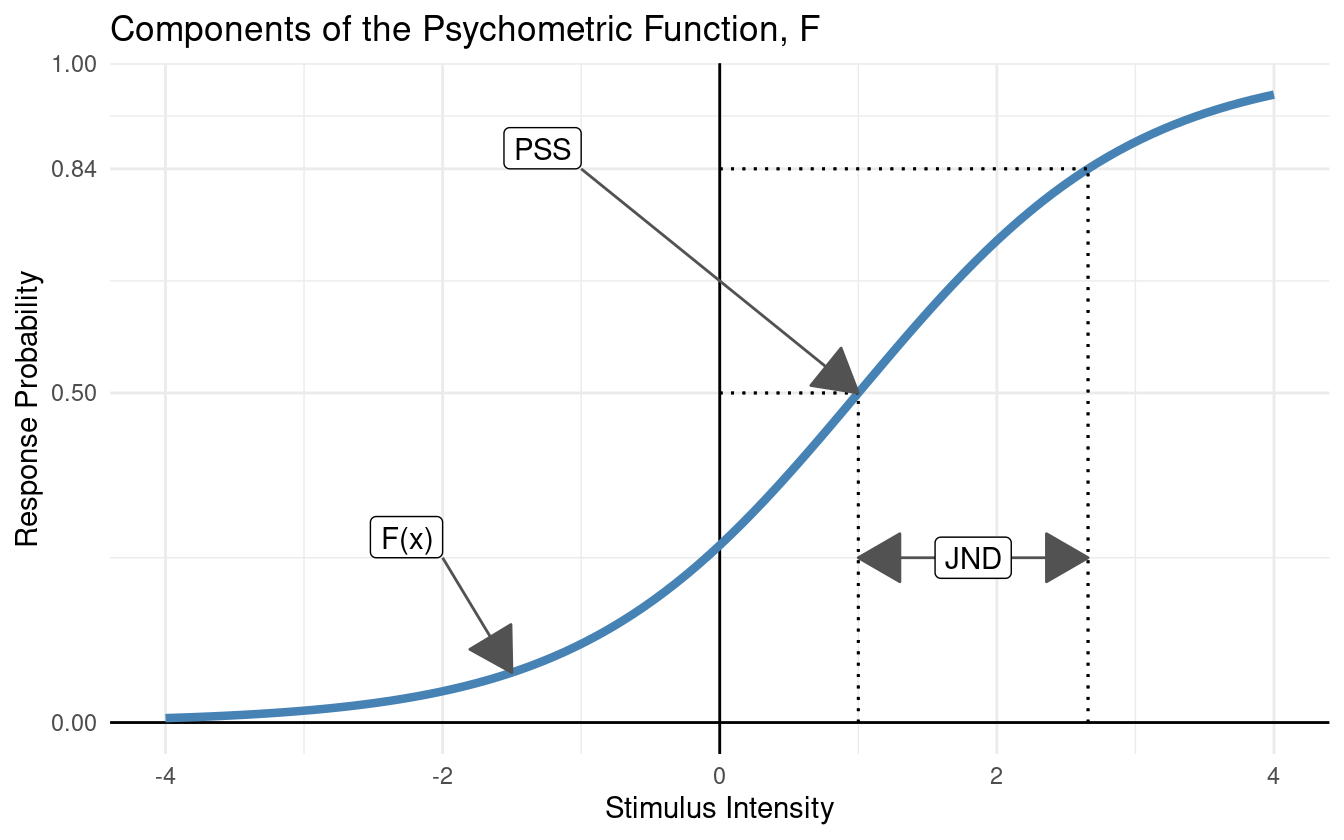
\includegraphics[width=0.85\linewidth]{020-psychometrics_files/figure-latex/ch020-plot-ref-pf-1} 

}

\caption{The PSS is defined as the point where an observer can do no better at determining temporal order than random guessing. The just noticeable difference is defined as the extra temporal delay between stimuli so that the temporal order is just able to be determined. Historically this has been defined as the difference between the 0.84 level and the PSS, though the upper level depends on domain expertise.}\label{fig:ch020-plot-ref-pf}
\end{figure}

Perceptual synchrony and temporal sensitivity can be modified through a baseline understanding. In order to perceive physical events as simultaneous, our brains must adjust for differences in temporal delays of transmission of both psychical signals and sensory processing \citep{fujisaki2004recalibration}. In some cases such as with audiovisual stimuli, the perception of simultaneity can be modified by repeatedly presenting the audiovisual stimuli at fixed time separations (called an adapter stimulus) to an observer \citep{vroomen2004recalibration}. This repetition of presenting the adapter stimulus is called \emph{temporal recalibration}.

The data set that I introduce in the next section concerns temporal order judgment across various sensory modalities with a temporal recalibration component.

\hypertarget{toj-task}{%
\section{Temporal Order Judgment Data}\label{toj-task}}

\emph{Which came first, the chicken or the experimentally controlled stimulus}

The data set that I am using in this paper comes from experiments done by A.N. Scurry and Dr.~F. Jiang in the Department of Psychology at the University of Nevada. Reduced temporal sensitivity in the aging population manifests in an impaired ability to perceive synchronous events as simultaneous, and similarly more difficulty in segregating asynchronous sensory signals that belong to different sources. The consequences of a widening of the temporal binding window is considered in \citet{scurry2019aging}, as well as a complete detailing of the experimental setup and recording process. A shortened summary of the methods is provided below.

There are four different tasks in the experiment: audio-visual, visual-visual, visual-motor, and duration, and I will refer to each task respectively as audiovisual, visual, sensorimotor, and duration. The participants consist of 15 young adults (age 20-27), 15 middle age adults (age 39-50), and 15 older adults (age 65-75), all recruited from the University of Nevada, Reno. Additionally all subjects are right handed and were reported to have normal or corrected to normal hearing and vision.

\begin{table}[!h]

\caption{\label{tab:ch020-multitask-data}Sample of motivating data.}
\centering
\begin{tabular}[t]{rrllllrl}
\toprule
soa & response & sid & task & trial & age\_group & age & sex\\
\midrule
-350 & 0 & O-m-BC & audiovisual & pre & older\_adult & 70 & M\\
-200 & 0 & M-m-SJ & duration & post1 & middle\_age & 48 & M\\
28 & 1 & O-f-KK & sensorimotor & pre & older\_adult & 66 & F\\
275 & 1 & O-f-MW & visual & post1 & older\_adult & 69 & F\\
\bottomrule
\end{tabular}
\end{table}

In the audiovisual TOJ task, participants were asked to determine the temporal order between an auditory and visual stimulus. Stimulus onset asynchrony values were selected uniformly between -500 to +500 ms with 50 ms steps, where negative SOAs indicated that the visual stimulus was leading, and positive values indicated that the auditory stimulus was leading. Each SOA value was presented 5 times in random order in the initial block. At the end of each trial the subject was asked to report if the auditory stimulus came before the visual, where a \(1\) indicates that they perceived the sound first, and a \(0\) indicates that they perceived the visual stimulus first.

A similar setup is repeated for the visual, sensorimotor, and duration tasks. The visual task presented two visual stimuli on the left and right side of a display with temporal asynchronies that varied between -300 ms to +300 ms with 25 ms steps. Negative SOAs indicated that the left stimulus was first, and positive that the right came first. A positive response indicates that the subject perceived the right stimulus first.

The sensorimotor task has subjects focus on a black cross on a screen. When it disappears, they respond by pressing a button. Additionally, when the cross disappears, a visual stimulus was flashed on the screen, and subjects were asked if they perceived the visual stimulus before or after their button press. The latency of the visual stimulus was partially determined by individual subject's average response time, so SOA values are not fixed between subjects and trials. A positive response indicates that the visual stimulus was perceived after the button press.

The duration task presents two vertically stacked circles on a screen with one appearing right after the other. The top stimulus appeared for a fixed amount of time of 300 ms, and the bottom was displayed for anywhere between +100 ms to +500 ms in 50 ms steps corresponding to SOA values between -200 ms to +200 ms. The subject then responds to if they perceived the bottom circle as appearing longer than the top circle.

\begin{table}[!h]

\caption{\label{tab:ch020-toj-summary}Summary of TOJ Tasks}
\centering
\begin{tabular}[t]{lll}
\toprule
Task & Positive Response & Positive SOA Truth\\
\midrule
Audiovisual & Perceived audio first & Audio came before visual\\
Visual & Perceived right first & Right came before left\\
Sensorimotor & Perceived visual first & Visual came before tactile\\
Duration & Perceived bottom as longer & Bottom lasted longer than top\\
\bottomrule
\end{tabular}
\end{table}

Finally, after the first block of each task was completed, the participants went through an adaptation period where they were presented with the respective stimuli from each task repeatedly at fixed temporal delays, then they repeated the task. To ensure that the adaptation affect persisted, the subject were presented with the adapter stimulus at regular intervals throughout the second block. The blocks are designated as \texttt{pre} and \texttt{post1}, \texttt{post2}, etc. in the data set. In this paper I will only be focusing on the \texttt{pre} and \texttt{post1} blocks.

\hypertarget{data-visualizations-and-quirks}{%
\section{Data Visualizations and Quirks}\label{data-visualizations-and-quirks}}

The dependent variable in these experiments is the perceived response which is encoded as a 0 or a 1, and the independent variable is the SOA value. If the response is plotted against the SOA values, then it is difficult to determine any relationship (see figure \ref{fig:ch020-simple-response-soa-plot}). Transparency can be used to better visualize the relationships between SOA value and responses. The center plot in figure \ref{fig:ch020-simple-response-soa-plot} uses the same data as the left plot, except that the transparency is set to 0.05. As a result, one can see that there is a higher density of ``0'' responses towards more negative SOAs, and a higher density of ``1'' responses for more positive SOAs. Taking it a step further, I can compute and plot the proportion of responses for a given SOA. This is displayed in the right panel. Now the relationship between SOA values and responses is clear -- as the SOA value goes from more negative to more positive, the proportion of positive responses increases from near 0 to near 1.

\begin{figure}

{\centering 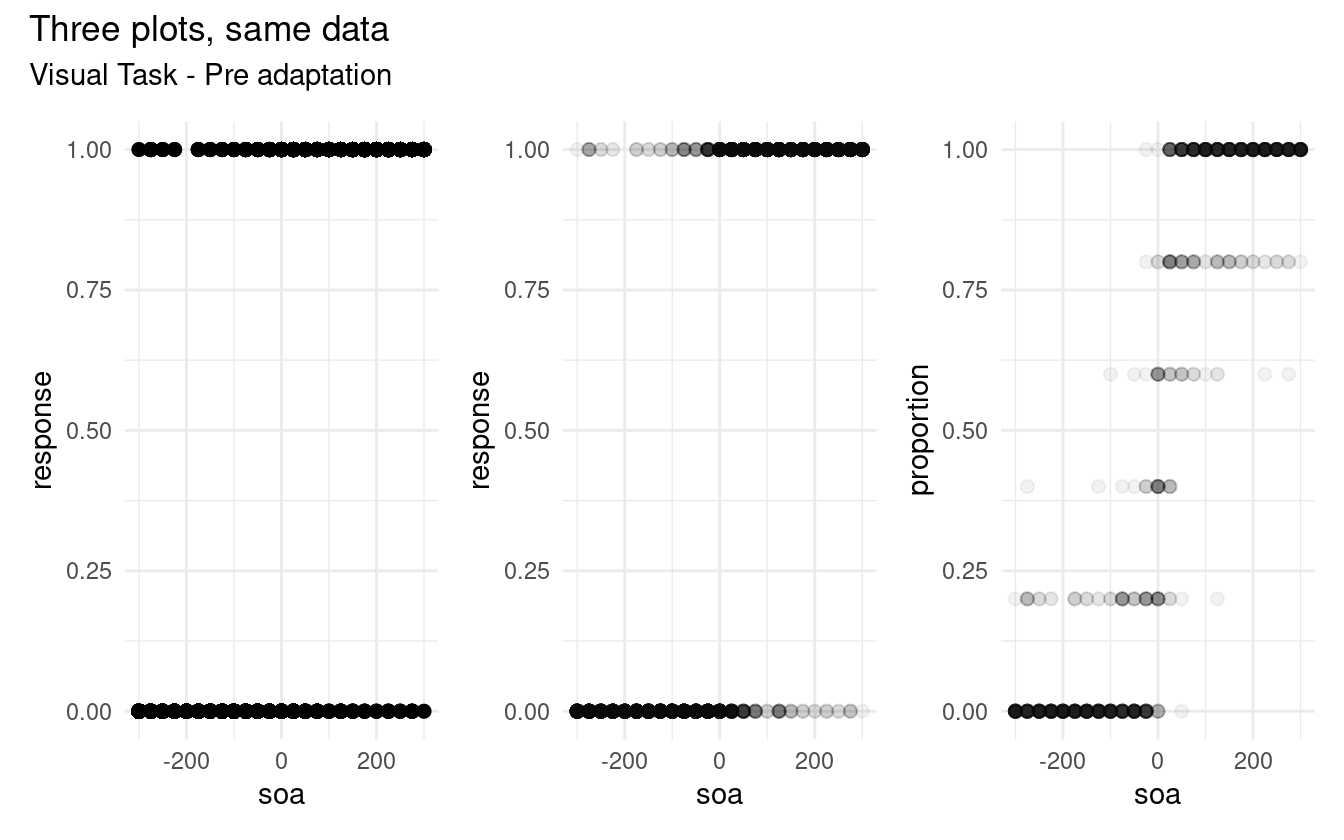
\includegraphics[width=0.85\linewidth]{020-psychometrics_files/figure-latex/ch020-simple-response-soa-plot-1} 

}

\caption{Left: Simple plot of response vs. soa value. Center: A plot of response vs. soa with transparency. Right: A plot of proportions vs. soa with transparency.}\label{fig:ch020-simple-response-soa-plot}
\end{figure}

Subjectively the right plot in figure \ref{fig:ch020-simple-response-soa-plot} is the easiest to interpret. Because of this, I will often present the observed and predicted data using the proportion of responses rather than the actual response. Proportional data also has the advantage of being bounded on the same interval as the response. For the audiovisual task, the responses can be aggregated into binomial data -- the number of positive responses for given SOA value -- which is sometimes more efficient to work with than the Bernoulli data (see table \ref{tab:ch020-av-bin-sample}). However the number of times an SOA is presented varies between the pre-adaptation and post-adaptation blocks; 5 and 3 times per SOA respectively.

\begin{table}[!h]

\caption{\label{tab:ch020-av-bin-sample}Audiovisual task with aggregated responses.}
\centering
\begin{tabular}[t]{lrrrr}
\toprule
trial & soa & n & k & proportion\\
\midrule
 & 200 & 5 & 4 & 0.80\\
\cmidrule{2-5}
 & 150 & 5 & 5 & 1.00\\
\cmidrule{2-5}
\multirow[t]{-3}{*}{\raggedright\arraybackslash pre} & -350 & 5 & 0 & 0.00\\
\cmidrule{1-5}
 & 350 & 3 & 3 & 1.00\\
\cmidrule{2-5}
 & -500 & 3 & 1 & 0.33\\
\cmidrule{2-5}
\multirow[t]{-3}{*}{\raggedright\arraybackslash post1} & -200 & 3 & 0 & 0.00\\
\bottomrule
\end{tabular}
\end{table}

Other quirks about the data pertain to the subjects. There is one younger subject that did not complete the audiovisual task, and one younger subject that did not complete the duration task. Additionally there is one older subject who's response data for the post-adaptation audiovisual task is unreasonable\footnote{By unreasonable, I mean that it is extremely unlikely that the data represents genuine responses.} (see figure \ref{fig:ch020-av-post1-O-f-CE-plot}).

\begin{figure}

{\centering 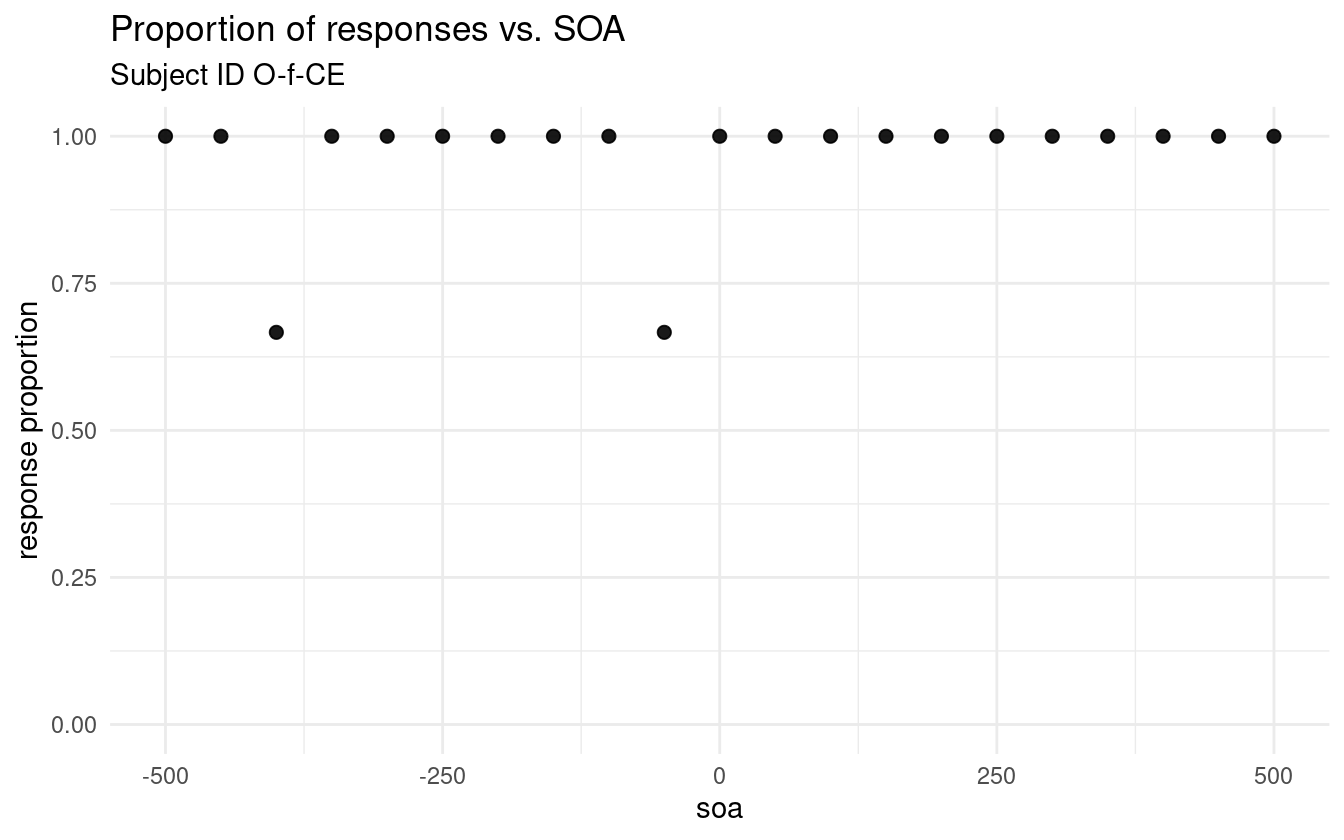
\includegraphics[width=0.85\linewidth]{020-psychometrics_files/figure-latex/ch020-av-post1-O-f-CE-plot-1} 

}

\caption{Post-adaptation response data for O-f-CE}\label{fig:ch020-av-post1-O-f-CE-plot}
\end{figure}

It is unreasonable because, of all the negative SOAs, there were only two correct responses\footnote{Correct in the sense that the perceived order matches the actual order.}. If a subject is randomly guessing the temporal order, then a naive estimate for the proportion of correct responses is 0.5. If a subject's proportion of correct responses is above 0.5, then they are doing better than random guessing. In figure \ref{fig:ch020-av-post-neg-trials} it is seen that subject O-f-CE is the only one who's proportion is below 0.5 (and by a considerable amount).

\begin{figure}

{\centering 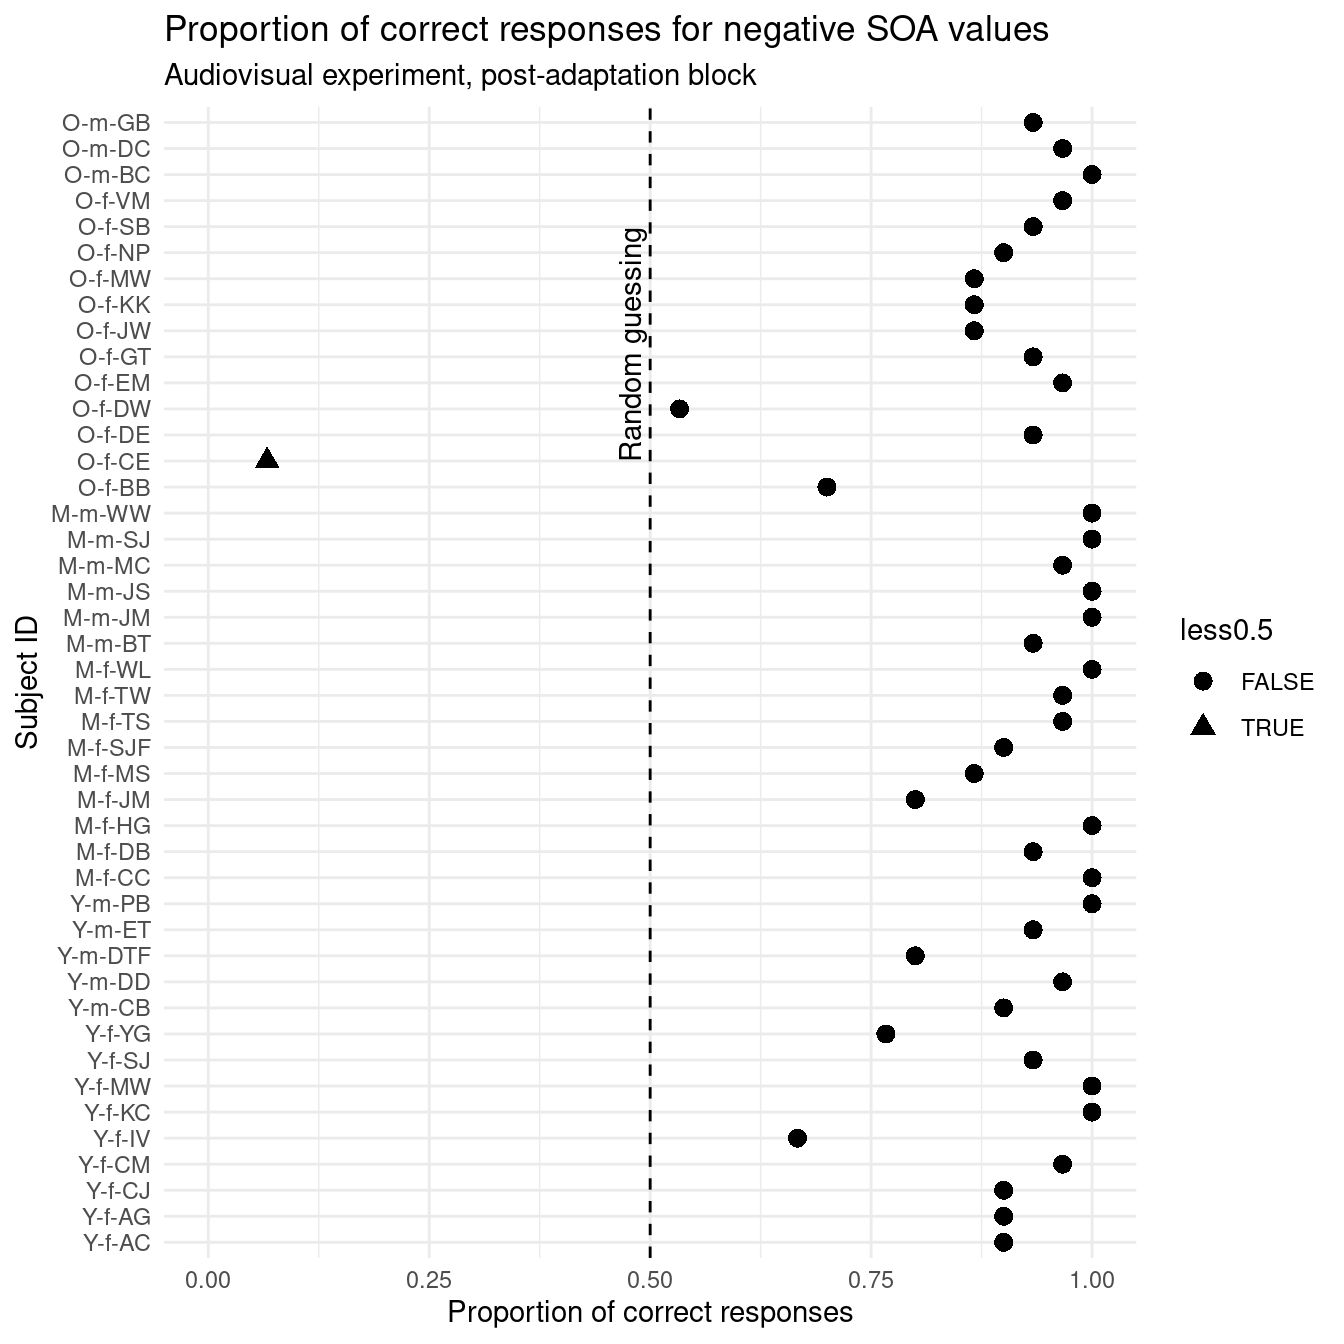
\includegraphics[width=0.85\linewidth]{020-psychometrics_files/figure-latex/ch020-av-post-neg-trials-1} 

}

\caption{Proportion of correct responses for negative SOA values during the post-adaptation audiovisual experiment.}\label{fig:ch020-av-post-neg-trials}
\end{figure}

The consequences of leaving in this experimental block in the data is considered in the \protect\hyperlink{results}{Chapter 6}, but it is a clear outlier that must be noted. When this method of detecting outliers is repeated for all tasks and blocks, then I end up with 17 records in total (see figure \ref{fig:ch020-naive-prop-outliers}), one of which is the aforementioned subject.

\begin{figure}

{\centering 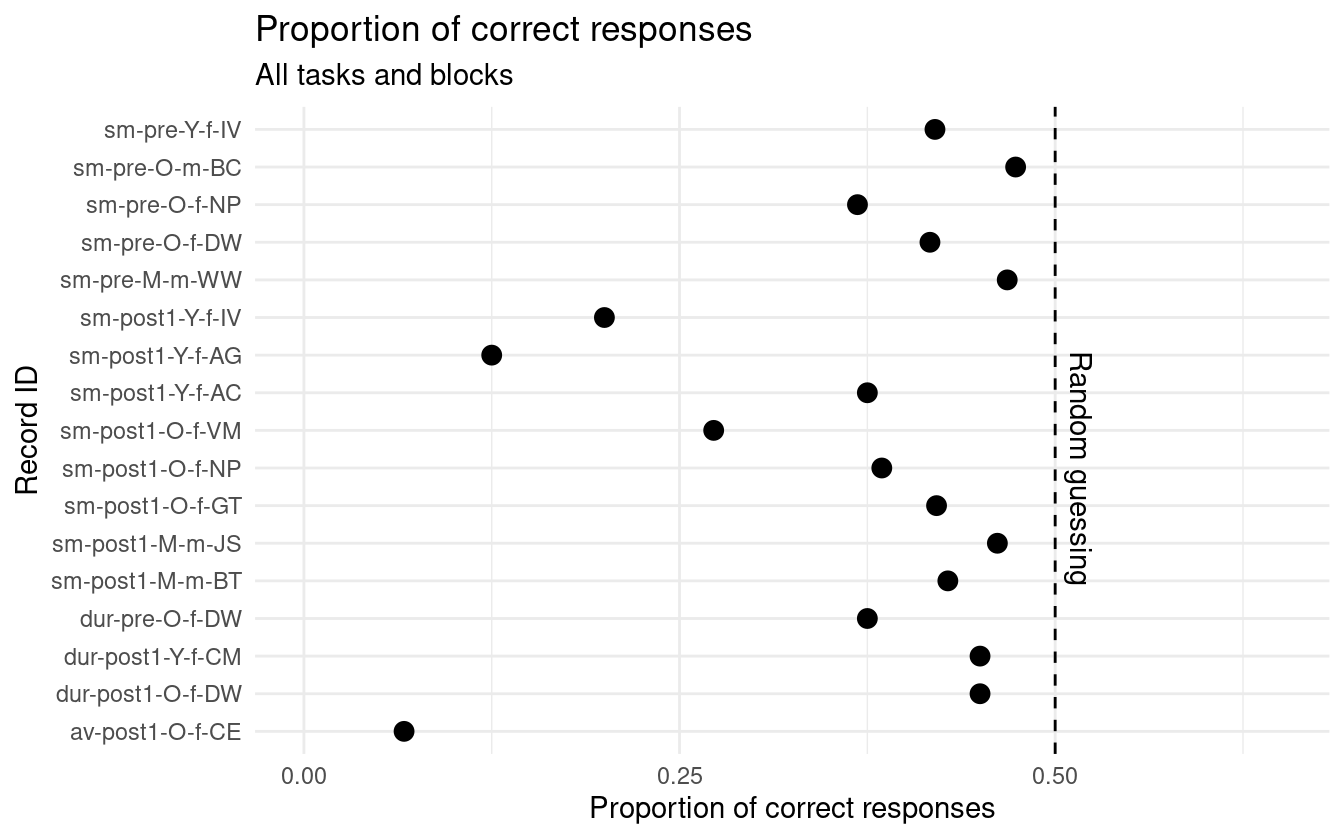
\includegraphics[width=0.85\linewidth]{020-psychometrics_files/figure-latex/ch020-naive-prop-outliers-1} 

}

\caption{Proportion of correct responses across all tasks and blocks Proportions are calculated individually for positive and negative SOAs.}\label{fig:ch020-naive-prop-outliers}
\end{figure}

Most of the records that are flagged by this method of outlier detection are from the sensorimotor task, and none are from the visual task. This may be attributed to the perceived difficulty of the task. One consequence of higher temporal sensitivity is that it is easier to determine temporal order. It may also be that determining temporal order is inherently easier for certain multisensory tasks compared to others. Since the sensorimotor task does not have fixed SOA values like the other tasks, it may be perceived as more difficult. Or perhaps the mechanisms that process tactile and visual signals are not as well coupled as those that process audio and visual signals. Once again, I'll consider the handling of the sensorimotor outliers in the results chapter.

Now that I have introduced the motivating data and some of the theory behind psychometric experiments, I am ready to introduce a Bayesian workflow for multilevel modeling of the psychometric function. If the reader is interested in a fun story, in the \protect\hyperlink{discussion}{discussion chapter} I talk about the process I went through to read in this psychometric data, clean it up, and produce a tidy data set that is ready for modeling. While data cleaning and transforming is a topic entirely to itself, it is not the main focus of this paper.

\hypertarget{workflow}{%
\chapter{Principled Bayesian Workflow}\label{workflow}}

\emph{The meat, the cheese, the entire sandwich}

Leading up to now, I haven't discussed what is a principled Bayesian workflow, nor what multilevel modeling is. I was hoping to build up the suspense. Well I hope you're now ready for the answer. A principled Bayesian workflow is a method of employing domain expertise and statistical knowledge to iteratively build a statistical model that satisfies the constraints and goals set forth by the researcher. Oh, and Bayesian techniques are used in exchange for classical ones. Maybe not worth the suspense, but the simple idea spawns a creative and descriptive way to analyze data.

What about the multilevel aspect? While I get into that more in the following sections, the concept is simple. Multilevel models should be the default. The alternatives are models with complete pooling, or models with no pooling. Pooling vs.~no pooling is a fancy way of saying that all the data is modeled as a whole, or the smallest component (group) is modeled individually. The former implies that the variation between groups is zero (all groups are the same), and the latter implies that the variation between groups is infinite (no groups are the same). Multilevel models assume that the truth is somewhere in the middle of zero and infinity. That's not a difficult thing to posit.

Hierarchical models are a specific kind of multilevel model where one or more groups are nested within a larger one. In the case of the psychometric data, there are three age groups, and within each age group are individual subjects. Multilevel modeling provides a way to quantify and apportion the variation within the data to each level in the model. For an in-depth introduction to multilevel modeling, see \citet{gelman2006data}.

There are many great resources out there for following along with an analysis of some data or problem, and much more is the abundance of tips, tricks, techniques, and testimonies to good modeling practices. The problem is that many of these prescriptions are given without context for when they are appropriate to be taken. According to \citet{betancourt2020}, this leaves ``practitioners to piece together their own model building workflows from potentially incomplete or even inconsistent heuristics.'' The concept of a principled workflow is that for any given problem, there is not, nor should there be, a default set of steps to take to get from data exploration to predictive inferences. Rather great consideration must be given to domain expertise and the questions that one is trying to answer with the data.

Since everyone asks different questions, the value of a model is not in how well it ticks the boxes of goodness-of-fit checks, but in how consistent it is with domain expertise and its ability to answer the unique set of questions. Betancourt suggests answering four questions to evaluate a model by:

\setstretch{1.0}

\begin{enumerate}
\def\labelenumi{\arabic{enumi}.}
\tightlist
\item
  Domain Expertise Consistency - Is our model consistent with our domain expertise?
\item
  Computational Faithfulness - Will our computational tools be sufficient to accurately fit our posteriors?
\item
  Inferential Adequacy - Will our inferences provide enough information to answer our questions?
\item
  Model Adequacy - Is our model rich enough to capture the relevant structure of the true data generating process?
\end{enumerate}

\setstretch{2.0}

Like any good Bayesian\footnote{The opposite of a Frequentist.}, much work is done before seeing the data or building a model. This may include talking with experts to gain domain knowledge or to \emph{elicit priors}. Experts may know something about a particular measure, perhaps the mean or variability of the data from years of research, and different experts may provide different estimates of a measure. The benefit of modeling in a Bayesian framework is that all prior knowledge may be incorporated into the model to be used to estimate the \emph{posterior distribution}. The same prior knowledge may also be used to check the posterior to ensure that predictions remain within physical or expert-given constraints. Consistency is key.

The computational tool I will be using to estimate the posterior is a probabilistic programming language (PPL) called Stan \citep{R-rstan} within the R programming language. Stan uses the No U-Turn Sampler (NUTS) version of Hamiltonian Monte Carlo (HMC) which I will discuss more in \protect\hyperlink{model-checking}{chapter 4}. For a gentle introduction to Bayesian statistics and sampling methods, see \citet{bolstad2016introduction}, and for an in-depth review of HMC see \citet{betancourt2017conceptual}.

The question of inferential adequacy depends on the set of questions that we are seeking to answer with the data from the psychometric experiment. The broad objective is to determine if there are any significant differences between age groups when it comes to temporal sensitivity, perceptual synchrony, and temporal recalibration, and if the task influences the results as well. The specific goals are to estimate and compare the PSS an JND across all age groups, conditions, and tasks, and determine the affect of recalibration between age groups.

For the last question, model adequacy, I will be following a set of steps proposed in \citet{betancourt2020}. The purpose of laying out these steps is not to again blindly check them off, but to force the analyst to carefully consider each point and make an \emph{informed} decision whether the step is necessary or to craft the specifics of how the step should be completed. The steps are listed in table \ref{tab:ch030-workflow-steps}. These steps are also not meant to be followed linearly. If at any point it is discovered that there is an issue in conceptual understanding or model adequacy or something else, then it is encouraged to go back to a previous step and start with a new understanding.

\begin{table}[!h]

\caption{\label{tab:ch030-workflow-steps}Principled workflow}
\centering
\begin{tabular}[t]{ll}
\toprule
Part & Step\\
\midrule
 & conceptual analysis\\
\cmidrule{2-2}
 & define observational space\\
\cmidrule{2-2}
\multirow[t]{-3}{*}{\raggedright\arraybackslash Pre-Model, Pre-Data} & construct summary statistics\\
\cmidrule{1-2}
 & develop model\\
\cmidrule{2-2}
 & construct summary functions\\
\cmidrule{2-2}
 & simulate Bayesian ensemble\\
\cmidrule{2-2}
 & prior checks\\
\cmidrule{2-2}
 & configure algorithm\\
\cmidrule{2-2}
 & fit simulated ensemble\\
\cmidrule{2-2}
 & algorithmic calibration\\
\cmidrule{2-2}
\multirow[t]{-8}{*}{\raggedright\arraybackslash Post-Model, Pre-Data} & inferential calibration\\
\cmidrule{1-2}
 & fit observed data\\
\cmidrule{2-2}
 & diagnose posterior fit\\
\cmidrule{2-2}
 & posterior retrodictive checks\\
\cmidrule{2-2}
\multirow[t]{-4}{*}{\raggedright\arraybackslash Post-Model, Post-Data} & celebrate\\
\bottomrule
\end{tabular}
\end{table}

I'll talk about each step in the first iteration, but may choose to omit steps in subsequent iterations if there are no changes. For the purposes of building a model and being concise, I will focus around the audiovisual TOJ task in this chapter, but the final model will apply similarly to the visual and duration tasks. For the sensorimotor task, the model will be modified to accept Bernoulli data as opposed to aggregated Binomial counts (described more in the next section).

\hypertarget{iter1}{%
\section{Iteration 1 (journey of a thousand miles)}\label{iter1}}

\textbf{Pre-Model, Pre-Data}

I begin the modeling process by modeling the experiment according to the description of how it occurred and how the data were collected. This first part consists of conceptual analysis, defining the observational space, and constructing summary statistics that can help us to identify issues in the model specification.

\emph{Conceptual Analysis}

In section \ref{toj-task} I discussed the experimental setup and data collection. To reiterate, subjects are presented with two stimuli separated by some temporal delay, and they are asked to respond as to their perception of the temporal order. There are 45 subjects with 15 each in the young, middle, and older age groups. As the SOA becomes larger in the positive direction, subjects are expected to give more ``positive'' responses, and as the SOA becomes larger in the negative direction, more ``negative'' responses are expected. By the way the experiment and responses are constructed, there is no expectation to see a reversal of this trend unless there was an issue with the subject's understanding of the directions given to them or an error in the recording device.

After the first experimental block the subjects go through a recalibration period, and repeat the experiment again. The interest is in seeing if the recalibration has an effect on temporal sensitivity and perceptual synchrony, and if the effect is different for each age group.

\emph{Define Observational Space}

The response that subjects give during a TOJ task is recorded as a zero or a one (see section \ref{toj-task}), and their relative performance is determined by the SOA value. Let \(y\) represent the binary outcome of a trial and let \(x\) be the SOA value.

\setstretch{1.0}

\begin{align*}
y_i &\in \lbrace 0, 1\rbrace \\
x_i &\in \mathbb{R}
\end{align*}
\setstretch{2.0}

If the SOA values are fixed like in the audiovisual task, then the responses can be aggregated into binomial counts, \(k\).

\setstretch{1.0}

\[
k_i, n_i \in \mathbb{Z}_0^+, k_i \le n_i
\]
\setstretch{2.0}

In the above expression, \(\mathbb{Z}_0^+\) represents the set of non-negative integers. Notice that the number of trials \(n\) has an index variable \(i\). This is because the number of trials per SOA is not fixed between blocks. In the pre-adaptation block, there are five trials per SOA compared to three in the post-adaptation block. So if observation 32 is recorded during a ``pre'' block, \(n_{32} = 5\), and if observation 1156 is during a ``post'' block, \(n_{1156} = 3\). Of course this is assuming that each subject completed all trials in the block, but the flexibility of the indexing can manage even if they didn't.

Then there are also three categorical variables -- age group, subject ID, and trial (block). The first two are treated as factor variables\footnote{Factor variables also go by the name index variable or categorical variable}. Rather than using one-hot encoding or dummy variables, the age levels are left as categories and a coefficient is fit for each level. Among the benefits of this approach is the ease of interpretation and ease of working with the data programmatically. This is especially true at the subject level. If a dummy variables was used for all 45 subjects, we would have 44 different dummy variables to work with times the number of coefficients that make estimates at the subject level. The number of parameters in the model grows rapidly as the model complexity grows.

Age groups and individual subjects can be indexed in the same way that number of trials is indexed. \(S_i\) refers to the subject in record \(i\), and similarly \(G_i\) refers to the age group of that subject. Observation 63 is for record ID av-post1-M-f-HG, so then \(S_{63}\) is M-f-HG and \(G_{63}\) is middle\_age. Under the hood of R, these factor levels are represented as integers (e.g.~middle age group level is stored internally as the number 2).

\setstretch{1.0}

\begin{Shaded}
\begin{Highlighting}[]
\NormalTok{(x <-}\StringTok{ }\KeywordTok{factor}\NormalTok{(}\KeywordTok{c}\NormalTok{(}\StringTok{"a"}\NormalTok{, }\StringTok{"a"}\NormalTok{, }\StringTok{"b"}\NormalTok{, }\StringTok{"c"}\NormalTok{)))}
\CommentTok{#> [1] a a b c}
\CommentTok{#> Levels: a b c}
\KeywordTok{storage.mode}\NormalTok{(x)}
\CommentTok{#> [1] "integer"}
\end{Highlighting}
\end{Shaded}

\setstretch{2.0}

This data storage representation can later be exploited for the Stan model.

The pre- and post-adaptation categories are treated as a binary indicator referred to as \(trt\) (short for treatment) since there are only two levels in the category. In this setup, a value of 1 indicates a post-adaptation block. I chose this encoding over the reverse because the pre-adaptation block is like the baseline performance, and it seemed more appropriate to interpret the post-adaptation block as turning on some effect. Using a binary indicator in a regression setting may not be the best practice as I discuss in section \ref{iter2}.

In the Stan modeling language, data for a binomial model with subject and age group levels and treatment is specified as

\setstretch{1.0}

\begin{verbatim}
data {
  int N;        // Number of observations
  int N_S;      // Number of subject levels
  int N_G;      // Number of age group levels
  int N_T;      // Number of treatment/control groups
  int n[N];     // Trials per SOA
  int k[N];     // binomial counts
  vector[N] x;  // SOA values
  int S[N];     // Subject identifier
  int G[N];     // Age group identifier
  int trt[N];   // Treatment indicator
}
\end{verbatim}

\setstretch{2.0}

In Stan (and unlike in R), data types must be statically declared. While sometimes a nuisance, this requirement aids in something called \emph{type inference}, and also lets Stan optimize certain parts of the model.

\emph{Construct Summary Statistics}

In order to effectively challenge the validity of the model, a set of summary statistics are constructed that help answer the questions of domain expertise consistency and model adequacy. We are studying the affects of age and temporal recalibration through the PSS and JND (see section \ref{psycho-experiments}), so it is natural to define summary statistics around these quantities to verify model consistency. Additionally the PSS and JND can be computed regardless of the model parameterization or chosen psychometric function.

By the experimental setup and recording process, it is impossible that a properly conducted block would result in a JND less than 0 (i.e.~the psychometric function is always non-decreasing), so that can be a lower limit for its threshold. On the other end it is unlikely that it will be beyond the limits of the SOA values, but even more concrete, it seems unlikely (though not impossible) that the just noticeable difference would be more than a second.

The lower bound on the JND can be further refined if we draw information from other sources. Some studies show that we cannot perceive time differences below 30 ms, and others show that an input lag as small as 100ms can impair a person's typing ability. Then according to these studies, a time delay of 100ms is enough to notice, and so a just noticeable difference should be much less than one second -- much closer to 100ms. I'll continue to use one second as an extreme estimate indicator, but will incorporate this knowledge when it comes to selecting priors.

As for the point of subjective simultaneity, it can be either positive or negative, with the belief that larger values are more rare. Some studies suggest that for audio-visual TOJ tasks, the separation between stimuli need to be as little as 20 milliseconds for subjects to be able to determine which modality came first \citep{vatakis2007influence}. Other studies suggest that our brains can detect temporal differences as small as 30 milliseconds. If these values are to be believed then we should be skeptical of PSS estimates larger than say 150 milliseconds in absolute value, just to be safe.

A histogram of computed PSS and JND values will suffice for summary statistics. We can estimate the proportion of values that fall outside of our limits defined above, and use them as indications of problems with the model fitting or conceptual understanding.

\textbf{Post-Model, Pre-Data}

It is now time to define priors for the model, while still not having looked at the {[}distribution of{]} data. The priors should be motivated by domain expertise and \emph{prior knowledge}, not the data. There are also many choices when it comes to selecting a psychometric (sigmoid) function. Common ones are logistic, Gaussian, and Weibull.

\begin{figure}

{\centering \includegraphics[width=0.85\linewidth]{030-workflow_files/figure-latex/ch031-pf-assortment-1} 

}

\caption{Assortment of psychometric functions.}\label{fig:ch031-pf-assortment}
\end{figure}

The Weibull psychometric function is more common when it comes to 2-AFC psychometric experiments where the independent variable is a stimulus intensity (non-negative) and the goal is signal detection. The data in this paper includes both positive and negative SOA values, so the Weibull is not a natural choice. In fact, because this is essentially a model for logistic regression, my first choice is the logistic function as it is the canonical choice for Binomial data. Additionally, the data in this study are reversible. The label of a positive response can be swapped with the label of a negative response and the inferences should remain the same. Since there is no natural ordering, it makes more sense for the psychometric function to be symmetric, e.g.~the logistic and Gaussian. I use symmetric loosely to mean that probability density function (PDF) is symmetric about its middle. More specifically, the distribution has zero skewness.

In practice, there is little difference in inference between the \emph{logit} and \emph{probit} links, but computationally the logit link is more efficient. I am also more familiar with working on the log-odds scale compared to the probit scale, so I make the decision to go forward with the logistic function. In \protect\hyperlink{model-checking}{chapter 4} I will show how even with a mis-specified link function, we can still achieve accurate predictions.

\emph{Develop Model}

Before moving on to specifying priors, I think it is appropriate to provide a little more background into generalized linear models (GLMs) and their role in working with psychometric functions. A GLM allows the linear model to be related to the outcome variable via a \emph{link} function. An example of this is the logit link - the inverse of the logistic function. The logistic function, \(F\), takes \(x \in \mathbb{R}\) and constrains the output to be in \((0, 1)\).

\setstretch{1.0}

\begin{equation}
  F(\theta) = \frac{1}{1 + \exp\left(-\theta\right)}
  \label{eq:logistic}
\end{equation}
\setstretch{2.0}

Since \(F\) is a strictly increasing and continuous function, it has an inverse, and the link for \eqref{eq:logistic} is the log-odds or logit function.

\setstretch{1.0}

\begin{equation}
  F^{-1}(\pi) = \mathrm{logit}(\pi) = \ln\left(\frac{\pi}{1 - \pi}\right)
  \label{eq:logit}
\end{equation}
\setstretch{2.0}

By taking \((F^{-1} \circ F)(\theta)\) we can arrive at a relationship that is linear in \(\theta\).

\setstretch{1.0}

\begin{align*}
  \pi = F(\theta) \Longleftrightarrow F^{-1}(\pi) &= F^{-1}(F(\theta)) \\
  & = \ln\left(\frac{F(\theta)}{1 - F(\theta)}\right) \\
  &= \ln(F(\theta)) - \ln(1 - F(\theta)) \\
  &= \ln\left(\frac{1}{1 + \exp(-\theta)}\right) - \ln\left(\frac{\exp(-\theta)}{1 + \exp(-\theta)}\right) \\
  &= - \ln(1 + \exp(-\theta)) - \ln(\exp(-\theta)) + \ln(1 + \exp(-\theta)) \\
  &= - \ln(\exp(-\theta)) \\
  &= \theta
\end{align*}
\setstretch{2.0}

The purpose of all this setup is to show that a model for the psychometric function can be specified using a linear predictor, \(\theta\). Given a simple slope-intercept model, one would typically write the linear predictor as

\setstretch{1.0}

\begin{equation}
  \theta = \alpha + \beta x
  \label{eq:linearform1}
\end{equation}
\setstretch{2.0}

This isn't the only acceptable form; it could be written in the centered parameterization

\setstretch{1.0}

\begin{equation}
  \theta = \beta(x - a)
  \label{eq:linearform2}
\end{equation}
\setstretch{2.0}

Both parameterizations will describe the same geometry, so why should it matter which form is chosen? Clearly the interpretation of the parameters change between the two models, but the reason becomes clear when you consider how the linear model relates back to the physical properties that the psychometric model describes. Take equation \eqref{eq:linearform1}, substitute it in to \eqref{eq:logistic}, and then take the logit of both sides

\setstretch{1.0}

\begin{equation}
  \mathrm{logit}(\pi) = \alpha+\beta x
  \label{eq:pfform1}
\end{equation}
\setstretch{2.0}

Now recall that the PSS is defined as the SOA values such that the response probability, \(\pi\), is \(0.5\). Substituting \(\pi = 0.5\) into \eqref{eq:pfform1} and solving for \(x\) yields

\setstretch{1.0}

\[
pss = -\frac{\alpha}{\beta}
\]
\setstretch{2.0}

Similarly, the JND is defined as the difference between the SOA value at the 84\% level and the PSS. Substituting \(\pi = 0.84\) into \eqref{eq:pfform1}, solving for \(x\), and subtracting off the pss yields

\setstretch{1.0}

\begin{equation}
  jnd = \frac{\mathrm{logit}(0.84)}{\beta}
  \label{eq:jnd1}
\end{equation}
\setstretch{2.0}

From the conceptual analysis, it is easy to define priors for the PSS and JND, but then how does one set the priors for \(\alpha\) and \(\beta\)? Let's say the prior for the just noticeable difference is \(jnd \sim \pi_j\). Then the prior for \(\beta\) would be

\setstretch{1.0}

\[
\beta \sim \frac{\mathrm{logit}(0.84)}{\pi_j}
\]
\setstretch{2.0}

The log-normal distribution has a nice property where its multiplicative inverse is still a log-normal distribution. We could let \(\pi_j = \mathrm{Lognormal}(\mu, \sigma^2)\) and then \(\beta\) would be distributed as

\setstretch{1.0}

\[
\beta \sim \mathrm{Lognormal}(-\mu + \ln(\mathrm{logit}(0.84)), \sigma^2)
\]
\setstretch{2.0}

This is acceptable, as it was determined last chapter that the slope must always be positive, and a log-normal distribution constrains the support to postive real numbers. Next suppose that the prior distribution for the PSS is \(pss \sim \pi_p\). Then the prior for \(\alpha\) is

\setstretch{1.0}

\[
\alpha \sim -\pi_p \cdot \beta
\]
\setstretch{2.0}

If \(\pi_p\) is set to a log-normal distribution as well, then \(\pi_p \cdot \beta\) would also be log-normal, but there is still the problem of the negative sign. If \(\alpha\) is always negative, then the PSS will also always be negative, which is certainly not always true. Furthermore, I don't want to \emph{a priori} put more weight on positive PSS values compared to negative ones, for which a log-normal distribution would not do.

Let's now go back and consider using equation \eqref{eq:linearform2} and repeat the above process.

\setstretch{1.0}

\begin{equation}
  \mathrm{logit}(\pi) = \beta(x - a)
  \label{eq:pfform2}
\end{equation}
\setstretch{2.0}

The just noticeable difference is still given by \eqref{eq:jnd1} and so the same method for choosing a prior can be used, but the PSS is now given by

\setstretch{1.0}

\[
pss = \alpha
\]
\setstretch{2.0}

This is a fortunate consequence of using \eqref{eq:linearform2} because now the JND only depends on \(\beta\) and the PSS only depends on \(\alpha\), and now \(\alpha\) can literally be interpreted as the PSS of the estimated psychometric function! Also thrown in is the ability to set a prior for \(\alpha\) that is symmetric around \(0\) like a Gaussian distribution.

This also brings me to point out the first benefit of using a modeling language like Stan over others. For fitting GLMs in R, there are a handful of functions that utilize MLE like \texttt{stats::glm} and others that use Bayesian methods like \texttt{rstanarm::stan\_glm} and \texttt{arm::bayesglm} \citep{R-rstanarm, R-arm}. Each of these functions requires the linear predictor to be in the form of \eqref{eq:linearform1}. The \texttt{stan\_glm} function actually uses Stan in the backend to fit a model, but is limited to priors from the Student t family of distributions. By writing the model directly in Stan, the linear model can be parameterized in any way and with any prior distribution, and so allows for much more expressive modeling - a key aspect of this principled workflow.

For the first iteration of this model, I am going to start with the simplest model that captures the structure of the data without including information about age group, treatment, or subject. Here is a simple model that draws information from the conceptual analysis.

\setstretch{1.0}

\begin{align*}
  k_i &\sim \mathrm{Binomial}(n_i, p_i) \\
  \mathrm{logit}(p_i) &= \beta ( x_i - \alpha )
\end{align*}
\setstretch{2.0}

Since I am using the linear model from \eqref{eq:linearform2}, setting the priors for \(\alpha\) and \(\beta\) is relatively straightforward. The PSS can be positive or negative without any expected bias towards either, so a symmetric distribution like the Gaussian is a fine choice for \(\alpha\) without having any other knowledge about the distribution of PSS values. Since I said earlier that a PSS value more than 150ms in absolute value is unlikely, I can define a Gaussian prior such that \(P(|pss| > 0.150) \approx 0.01\). Since the prior does not need to be exact, the following mean and variance suffice:

\setstretch{1.0}

\[
pss \sim \mathcal{N}(0, 0.06^2) \Longleftrightarrow \alpha \sim \mathcal{N}(0, 0.06^2)
\]
\setstretch{2.0}

For the just noticeable difference, I will continue to use the log-normal distribution because it is constrained to positive values and has the nice reciprocal property. The JND is expected to be close to 100ms and extremely unlikely to exceed 1 second. This implies a prior such that the mean is around 100ms and the bulk of the distribution is below 1 second - i.e.~\(E[X] \approx 0.100\) and \(P(X < 1) \approx 0.99\). This requires solving a system of nonlinear equations in two variables

\setstretch{1.0}

\[
\begin{cases}
E[X] = 0.100 = \exp\left(\mu + \sigma^2 / 2\right) \\
P(X < 1) = 0.99 = 0.5 + 0.5 \cdot \mathrm{erf}\left[\frac{\ln (1) - \mu}{\sqrt{2} \cdot \sigma}\right]
\end{cases}
\]
\setstretch{2.0}

This nonlinear system can be solved using Stan's algebraic solver.

\setstretch{1.0}

\begin{verbatim}
functions {
  vector system(vector y, vector theta, real[] x_r, int[] x_i) {
    vector[2] z;
    z[1] = exp(y[1] + y[2]^2 / 2) - theta[1];
    z[2] = 0.5 + 0.5 * erf(-y[1] / (sqrt(2) * y[2])) - theta[2];
    return z;
  }
}
transformed data {
  vector[2] y_guess = [1, 1]';
  real x_r[0];
  int x_i[0];
}
transformed parameters {
  vector[2] theta = [0.100, 0.99]';
  vector[2] y;
  y = algebra_solver(system, y_guess, theta, x_r, x_i);
}
\end{verbatim}

\setstretch{2.0}

\setstretch{1.0}

\begin{Shaded}
\begin{Highlighting}[]
\NormalTok{fit <-}\StringTok{ }\KeywordTok{sampling}\NormalTok{(prior_jnd, }
                \DataTypeTok{iter=}\DecValTok{1}\NormalTok{, }\DataTypeTok{warmup=}\DecValTok{0}\NormalTok{, }\DataTypeTok{chains=}\DecValTok{1}\NormalTok{, }\DataTypeTok{refresh=}\DecValTok{0}\NormalTok{,}
                \DataTypeTok{seed=}\DecValTok{31}\NormalTok{, }\DataTypeTok{algorithm=}\StringTok{"Fixed_param"}\NormalTok{)}
\NormalTok{sol <-}\StringTok{ }\KeywordTok{extract}\NormalTok{(fit)}
\NormalTok{sol}\OperatorTok{$}\NormalTok{y}
\CommentTok{#>           }
\CommentTok{#> iterations   [,1]  [,2]}
\CommentTok{#>       [1,] -7.501 3.225}
\end{Highlighting}
\end{Shaded}

\setstretch{2.0}

The solver has determined that \(\mathrm{Lognormal}(-7.5, 3.2^2)\) is the appropriate prior. However, simulating some values from this distribution produces a lot of extremely small values (\(<10^{-5}\)) and a few extremely large values (\(\approx 10^2\)). This is because the expected value of a log-normal random variable depends on both the mean and standard deviation. If the median is used in place for the mean, then a more acceptable prior may be determined.

\setstretch{1.0}

\begin{Shaded}
\begin{Highlighting}[]
\NormalTok{fit <-}\StringTok{ }\KeywordTok{sampling}\NormalTok{(prior_jnd_using_median, }
                \DataTypeTok{iter=}\DecValTok{1}\NormalTok{, }\DataTypeTok{warmup=}\DecValTok{0}\NormalTok{, }\DataTypeTok{chains=}\DecValTok{1}\NormalTok{, }\DataTypeTok{refresh=}\DecValTok{0}\NormalTok{,}
                \DataTypeTok{seed=}\DecValTok{31}\NormalTok{, }\DataTypeTok{algorithm=}\StringTok{"Fixed_param"}\NormalTok{)}
\NormalTok{sol <-}\StringTok{ }\KeywordTok{extract}\NormalTok{(fit)}
\NormalTok{sol}\OperatorTok{$}\NormalTok{y}
\CommentTok{#>           }
\CommentTok{#> iterations   [,1]   [,2]}
\CommentTok{#>       [1,] -2.303 0.9898}
\end{Highlighting}
\end{Shaded}

\setstretch{2.0}

Sampling from a log-normal distribution with these parameters and plotting the histogram shows no inconsistency with the domain expertise.

\begin{center}\includegraphics[width=0.85\linewidth]{030-workflow_files/figure-latex/ch031-Risky-Lion-1} \end{center}

So now with a prior for the JND, the prior for \(\beta\) can be determined.

\setstretch{1.0}

\[
jnd \sim \mathrm{Lognormal}(-2.3, 0.99^2) \Longleftrightarrow \frac{1}{jnd} \sim \mathrm{Lognormal}(2.3, 0.99^2)
\]
\setstretch{2.0}

and

\setstretch{1.0}

\[
\beta = \frac{\mathrm{logit}(0.84)}{jnd} \sim \mathrm{Lognormal}(2.8, 0.99^2)
\]
\setstretch{2.0}

The priors do not need to be too exact. Rounding the parameters for \(\beta\), the simple model is

\setstretch{1.0}

\begin{align*}
  k_i &\sim \mathrm{Binomial}(n_i, p_i) \\
  \mathrm{logit}(p_i) &= \beta ( x_i - \alpha ) \\
  \alpha &\sim \mathcal{N}(0, 0.06^2) \\
  \beta &\sim \mathrm{Lognormal}(3, 1^2)
\end{align*}
\setstretch{2.0}

and in Stan, the model code is

\setstretch{1.0}

\begin{verbatim}
data {
  int N;
  int n[N];
  int k[N];
  vector[N] x;
}
parameters {
  real alpha;
  real<lower=0> beta;
}
model {
  vector[N] p = beta * (x - alpha);
  alpha ~ normal(0, 0.06);
  beta ~ lognormal(3.0, 1.0);
  k ~ binomial_logit(n, p);
}
generated quantities {
  vector[N] log_lik;
  vector[N] k_pred;
  vector[N] theta = beta * (x - alpha);
  vector[N] p = inv_logit(theta);
  for (i in 1:N) {
    log_lik[i] = binomial_logit_lpmf(k[i] | n[i], theta[i]);
    k_pred[i]  = binomial_rng(n[i], p[i]);
  }
}
\end{verbatim}

\setstretch{2.0}

Notice that the model block is nearly identical to the mathematical model!

\emph{Construct Summary Functions}

Whew! that was a lot of work to define the priors for just two parameters. Thankfully going forward not as much work will need to be done to expand the model. The next step is to construct any relevant summary functions. Since the distribution of posterior PSS and JND values are needed for the summary statistics, it will be nice to have a function that can take in the posterior samples for \(\alpha\) and \(\beta\) and return the PSS and JND values. I'll define \(Q\) as a more general function that takes in the two parameters and a probability, \(\pi\), and returns the distribution of SOA values at \(\pi\).

\setstretch{1.0}

\begin{equation}
  Q(\pi; \alpha, \beta) = \frac{\mathrm{logit(\pi)}}{\beta} + \alpha
  \label{eq:summfun1}
\end{equation}
\setstretch{2.0}

The function can be defined in R as

\setstretch{1.0}

\begin{Shaded}
\begin{Highlighting}[]
\NormalTok{Q <-}\StringTok{ }\ControlFlowTok{function}\NormalTok{(p, a, b) }\KeywordTok{qlogis}\NormalTok{(p) }\OperatorTok{/}\StringTok{ }\NormalTok{b }\OperatorTok{+}\StringTok{ }\NormalTok{a}
\end{Highlighting}
\end{Shaded}

\setstretch{2.0}

With \(Q\), the PSS and JND can be calculated as

\setstretch{1.0}

\begin{align}
  pss &= Q(0.5) \\
  jnd &= Q(0.84) - Q(0.5)
\end{align}
\setstretch{2.0}

\emph{Simulate Bayesian Ensemble}

During this step, I simulate the Bayesian ensemble and later feed the prior values into the summary functions in order to verify that there are no other inconsistencies with domain knowledge. Since the model is fairly simple, I will simulate directly in R.

\setstretch{1.0}

\begin{Shaded}
\begin{Highlighting}[]
\KeywordTok{set.seed}\NormalTok{(}\DecValTok{124}\NormalTok{)}
\NormalTok{n <-}\StringTok{ }\DecValTok{10000}

\NormalTok{a <-}\StringTok{ }\KeywordTok{rnorm}\NormalTok{(n, }\DecValTok{0}\NormalTok{, }\FloatTok{0.06}\NormalTok{)}
\NormalTok{b <-}\StringTok{ }\KeywordTok{rlnorm}\NormalTok{(n, }\FloatTok{3.0}\NormalTok{, }\DecValTok{1}\NormalTok{)}

\NormalTok{dat <-}\StringTok{ }\KeywordTok{with}\NormalTok{(av_dat, }\KeywordTok{list}\NormalTok{(}\DataTypeTok{N =}\NormalTok{ N, }\DataTypeTok{x =}\NormalTok{ x, }\DataTypeTok{n =}\NormalTok{ n)) }
\NormalTok{n_obs <-}\StringTok{ }\KeywordTok{length}\NormalTok{(dat}\OperatorTok{$}\NormalTok{x)}

\NormalTok{idx <-}\StringTok{ }\KeywordTok{sample}\NormalTok{(}\DecValTok{1}\OperatorTok{:}\NormalTok{n, n_obs, }\DataTypeTok{replace =} \OtherTok{TRUE}\NormalTok{)}
\NormalTok{probs <-}\StringTok{ }\KeywordTok{logistic}\NormalTok{(b[idx] }\OperatorTok{*}\StringTok{ }\NormalTok{(dat}\OperatorTok{$}\NormalTok{x }\OperatorTok{-}\StringTok{ }\NormalTok{a[idx]))}
\NormalTok{sim_k <-}\StringTok{ }\KeywordTok{rbinom}\NormalTok{(n_obs, dat}\OperatorTok{$}\NormalTok{n, probs)}
\end{Highlighting}
\end{Shaded}

\setstretch{2.0}

\emph{Prior Checks}

This step pertains to ensuring that prior estimates are consistent with domain expertise. I already did that in the model construction step by sampling values for the just noticeable difference. The first prior chosen was not producing JND estimates that were consistent with domain knowledge, so I adjusted accordingly. That check would normally be done during this step, and I would have had to return to the model development step.

Figure \ref{fig:ch031-prior-pf-plot} shows the distribution of prior psychometric functions derived from the simulated ensemble. There are a few very steep and very shallow curves, but the majority fall within a range that appears likely.

\begin{figure}

{\centering \includegraphics[width=0.85\linewidth]{030-workflow_files/figure-latex/ch031-prior-pf-plot-1} 

}

\caption{Prior distribution of psychometric functions using the priors for alpha and beta.}\label{fig:ch031-prior-pf-plot}
\end{figure}

Additionally most of the PSS values are within \(\pm 0.1\) with room to allow for some larger values. Let's check the prior distribution of PSS and JND values.

\begin{figure}

{\centering \includegraphics[width=0.85\linewidth]{030-workflow_files/figure-latex/ch031-prior-pss-plot-1} 

}

\caption{PSS prior distribution.}\label{fig:ch031-prior-pss-plot}
\end{figure}

\begin{figure}

{\centering \includegraphics[width=0.85\linewidth]{030-workflow_files/figure-latex/ch031-prior-jnd-plot-1} 

}

\caption{JND prior distribution.}\label{fig:ch031-prior-jnd-plot}
\end{figure}

I am satisfied with the prior coverage of the PSS and JND values, and there are only a few samples that go beyond the extremes that were specified in the summary statistics step.

\emph{Configure Algorithm}

There are a few parameters that can be set for Stan. On the user side, the main parameters are the number of iterations, the number of warm-up iterations, the target acceptance rate, and the number of chains to run. The NUTS algorithm samples in two phases: a warm-up phase and a sampling phase. During the warm-up phase, the sampler is automatically tuning three internal parameters that can significantly affect the sampling efficiency. By default, the Stan function will use half the number of iterations for warm-up and the other half for actual sampling. The full details of Stan's HMC algorithm is described in the Stan reference manual. For now I am going to use the default algorithm parameters in Stan, and will tweak them later if and when issues arise.

\emph{Fit Simulated Ensemble}

Nothing to say here. Only code.

\setstretch{1.0}

\begin{Shaded}
\begin{Highlighting}[]
\NormalTok{sim_dat <-}\StringTok{ }\KeywordTok{with}\NormalTok{(av_dat, }\KeywordTok{list}\NormalTok{(}\DataTypeTok{N =}\NormalTok{ N, }\DataTypeTok{x =}\NormalTok{ x, }\DataTypeTok{n =}\NormalTok{ n, }\DataTypeTok{k =}\NormalTok{ sim_k)) }
\NormalTok{m031 <-}\StringTok{ }\KeywordTok{sampling}\NormalTok{(m031_stan, }\DataTypeTok{data =}\NormalTok{ sim_dat, }
                 \DataTypeTok{chains =} \DecValTok{4}\NormalTok{, }\DataTypeTok{cores =} \DecValTok{4}\NormalTok{, }\DataTypeTok{refresh =} \DecValTok{0}\NormalTok{)}
\end{Highlighting}
\end{Shaded}

\setstretch{2.0}

\emph{Algorithmic Calibration}

One benefit of using HMC over other samplers like Gibbs sampling is that HMC offers diagnostic tools for the health of chains and the ability to check for \emph{divergent transitions} (discussed in \ref{divergent-transitions}). To check the basic diagnostics of the model, I run the following code.

\setstretch{1.0}

\begin{Shaded}
\begin{Highlighting}[]
\KeywordTok{check_hmc_diagnostics}\NormalTok{(m031)}
\CommentTok{#> }
\CommentTok{#> Divergences:}
\CommentTok{#> 0 of 4000 iterations ended with a divergence.}
\CommentTok{#> }
\CommentTok{#> Tree depth:}
\CommentTok{#> 0 of 4000 iterations saturated the maximum tree depth of 10.}
\CommentTok{#> }
\CommentTok{#> Energy:}
\CommentTok{#> E-BFMI indicated no pathological behavior.}
\end{Highlighting}
\end{Shaded}

\setstretch{2.0}

There is no undesirable behavior from this model, so next I check the summary statistics of the estimated parameters. The \(\hat{R}\) statistic is a comparison of the measure of variance within chains and between chains. When chains have converged to a stationary distribution, the variance within and between chains is the same, and the ratio is one. Values of \(\hat{R} > 1.1\) are usually indicative of chains that have not converged to a common distribution. Lastly there is the effective sample size (\(N_{\mathrm{eff}}\)) which is a loose measure for the autocorrelation within the parameter samples. As autocorrelation generally decreases as the lag increases, one can achieve a higher \(N_{\mathrm{eff}}\) by running a chain with more samples and then \emph{thinning} the samples, i.e.~saving only every \(n^{th}\) sample.

\begin{table}[!h]

\caption{\label{tab:ch031-Cloudy-Toupee}Summary statistics of the fitted Bayesian ensemble.}
\centering
\begin{tabular}[t]{lrrrrrrr}
\toprule
parameter & mean & se\_mean & sd & 2.5\% & 97.5\% & n\_eff & Rhat\\
\midrule
alpha & 0.0061 & 0.0001 & 0.0038 & -0.0012 & 0.0136 & 4039 & 0.9995\\
beta & 10.7681 & 0.0051 & 0.2404 & 10.3043 & 11.2313 & 2202 & 1.0003\\
\bottomrule
\end{tabular}
\end{table}

Both the \(\hat{R}\) and \(N_{\mathrm{eff}}\) look fine for both \(\alpha\) and \(\beta\), thought it is slightly concerning that \(\alpha\) is centered relatively far from zero. This could just be due to sampling variance, so I will continue on to the next step.

\textbf{Post-Model, Post-Data}

\emph{Fit Observed Data}

All of the work up until now has been done without peaking at the observed data. Satisfied with the model so far, I can now go ahead and run the data through.

\setstretch{1.0}

\begin{Shaded}
\begin{Highlighting}[]
\NormalTok{m031 <-}\StringTok{ }\KeywordTok{sampling}\NormalTok{(m031_stan, }\DataTypeTok{data =}\NormalTok{ obs_dat, }
                 \DataTypeTok{chains =} \DecValTok{4}\NormalTok{, }\DataTypeTok{cores =} \DecValTok{4}\NormalTok{, }\DataTypeTok{refresh =} \DecValTok{200}\NormalTok{)}
\end{Highlighting}
\end{Shaded}

\setstretch{2.0}

\emph{Diagnose Posterior Fit}

Here I repeat the diagnostic checks that I used after fitting the simulated Bayesian ensemble.

\setstretch{1.0}

\begin{Shaded}
\begin{Highlighting}[]
\KeywordTok{check_hmc_diagnostics}\NormalTok{(m031)}
\CommentTok{#> }
\CommentTok{#> Divergences:}
\CommentTok{#> 0 of 4000 iterations ended with a divergence.}
\CommentTok{#> }
\CommentTok{#> Tree depth:}
\CommentTok{#> 0 of 4000 iterations saturated the maximum tree depth of 10.}
\CommentTok{#> }
\CommentTok{#> Energy:}
\CommentTok{#> E-BFMI indicated no pathological behavior.}
\end{Highlighting}
\end{Shaded}

\setstretch{2.0}

\begin{table}[!h]

\caption{\label{tab:ch031-Maroon-Oyster}Summary statistics of the fitted Bayesian ensemble.}
\centering
\begin{tabular}[t]{lrrrrrrr}
\toprule
parameter & mean & se\_mean & sd & 2.5\% & 97.5\% & n\_eff & Rhat\\
\midrule
alpha & 0.0373 & 0.0001 & 0.0043 & 0.029 & 0.0458 & 3765 & 1.000\\
beta & 8.4259 & 0.0039 & 0.1839 & 8.070 & 8.7897 & 2249 & 1.001\\
\bottomrule
\end{tabular}
\end{table}

No indications of an ill-behaved posterior fit! Let's also check the posterior distribution of \(\alpha\) and \(\beta\) against the prior density (\ref{fig:ch031-m031-posterior-alpha-beta}).

\begin{figure}

{\centering 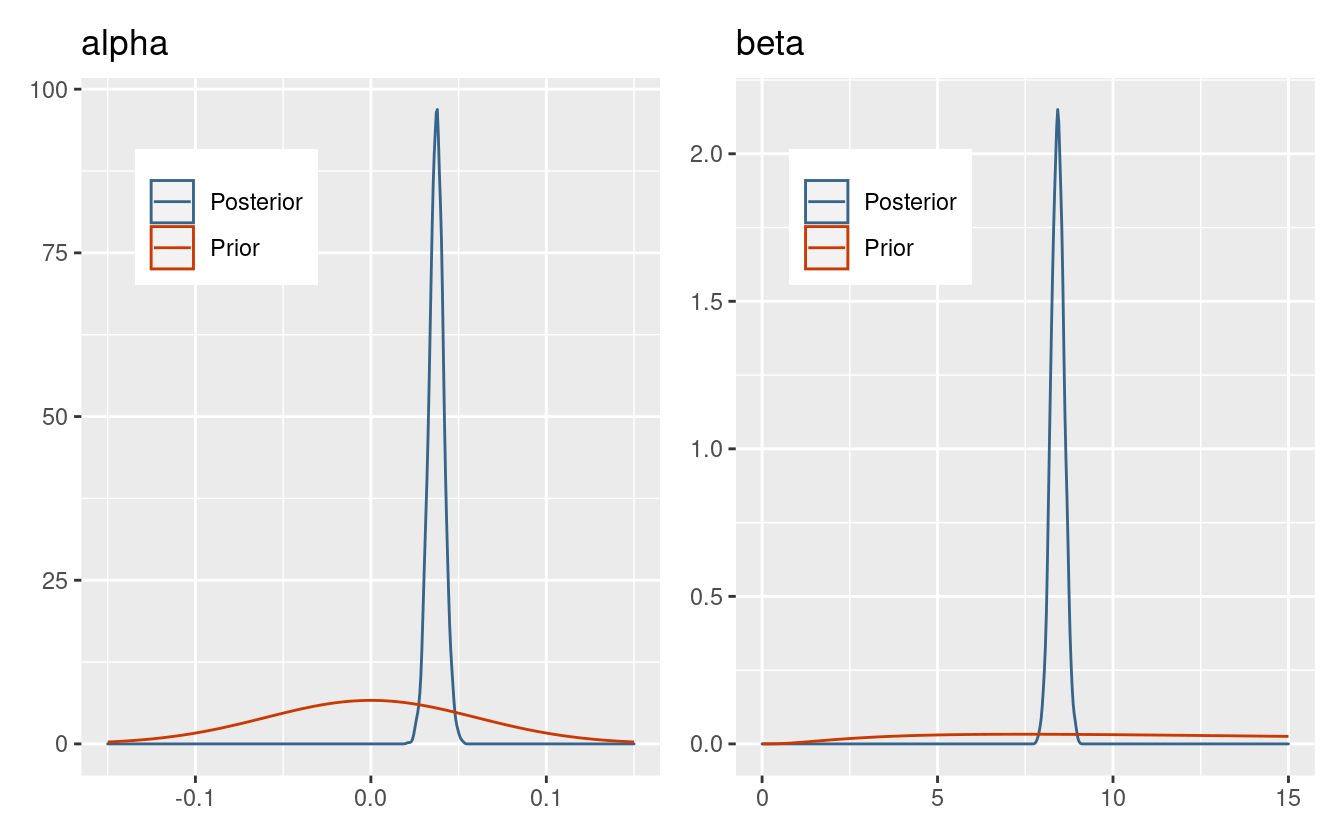
\includegraphics[width=0.85\linewidth]{030-workflow_files/figure-latex/ch031-m031-posterior-alpha-beta-1} 

}

\caption{Comparison of posterior distributions for alpha and beta to their respective prior distributions.}\label{fig:ch031-m031-posterior-alpha-beta}
\end{figure}

The posterior distributions for \(\alpha\) and \(\beta\) are well within the range determined by domain knowledge, and highly concentrated due to both the large amount of data and the fact that this is a completely pooled model - no stratification. As expected, the prior for the JND could have been tighter with more weight below half a second compared to the one second limit used, but this is not prior information, so it is not prudent to change the prior in this manner after having seen the posterior. As a rule of thumb, priors should only be updated as motivated by domain expertise and not by posterior distributions.

\emph{Posterior Retrodictive Checks}

Finally it is time to run the posterior samples through the summary functions and then perform \emph{retrodictive} checks. A retrodiction is using the posterior model to predict and compare to the observed data. This is simply done by drawing samples from the posterior and feeding in the observational data. This may be repeated to gain a retrodictive distribution.

\setstretch{1.0}

\begin{Shaded}
\begin{Highlighting}[]
\NormalTok{posterior_pss <-}\StringTok{ }\KeywordTok{Q}\NormalTok{(}\FloatTok{0.5}\NormalTok{, p031}\OperatorTok{$}\NormalTok{alpha, p031}\OperatorTok{$}\NormalTok{beta)}
\NormalTok{posterior_jnd <-}\StringTok{ }\KeywordTok{Q}\NormalTok{(}\FloatTok{0.84}\NormalTok{, p031}\OperatorTok{$}\NormalTok{alpha, p031}\OperatorTok{$}\NormalTok{beta) }\OperatorTok{-}\StringTok{ }\NormalTok{posterior_pss}
\end{Highlighting}
\end{Shaded}

\setstretch{2.0}

\begin{figure}

{\centering 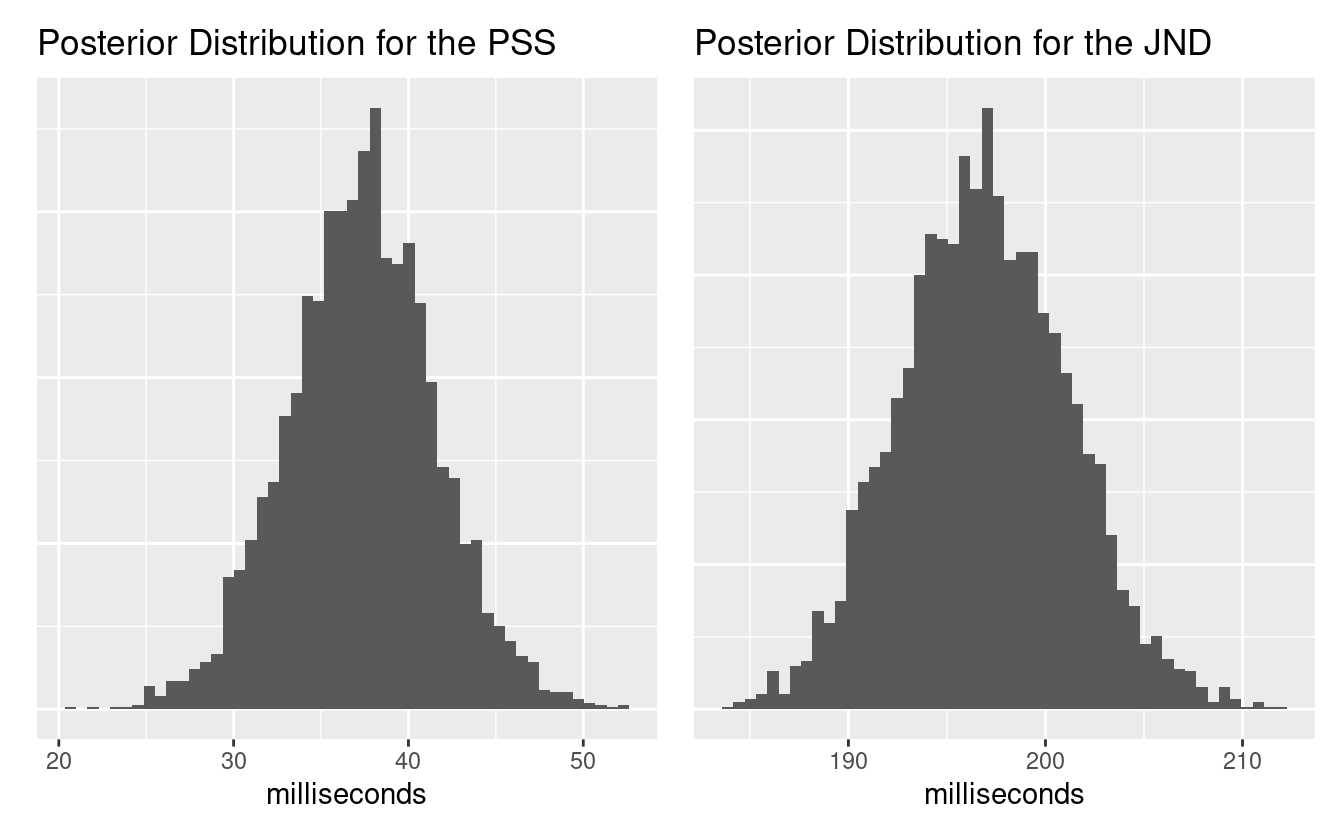
\includegraphics[width=0.85\linewidth]{030-workflow_files/figure-latex/ch031-posterior-pss-jnd-plot-1} 

}

\caption{Posterior distribution of the PSS and JND.}\label{fig:ch031-posterior-pss-jnd-plot}
\end{figure}

Neither of the posterior estimates for the PSS or JND exceed the extreme cutoffs set in the earlier steps, so I can be confident that the model is consistent with domain expertise. Let's also take a second to appreciate how simple it is to visualize and summarize the distribution of values for these measures. Using classical techniques like MLE might require using bootstrap methods to estimate the distribution of parameter values, or one might approximate the parameter distributions using the mean and standard error of the mean to simulate new values. Since we have the entire posterior distribution we can calculate the distribution of transformed parameters by working directly with the posterior samples and be sure that the intervals are credible.

Next is to actually do the posterior retrodictions. I will do this in two steps to better show how the distribution of posterior psychometric functions relates to the observed data, and then compare the observed data to the retrodictions. Figure \ref{fig:ch031-posterior-pf-plot} shows the result of the first step.

\begin{figure}

{\centering 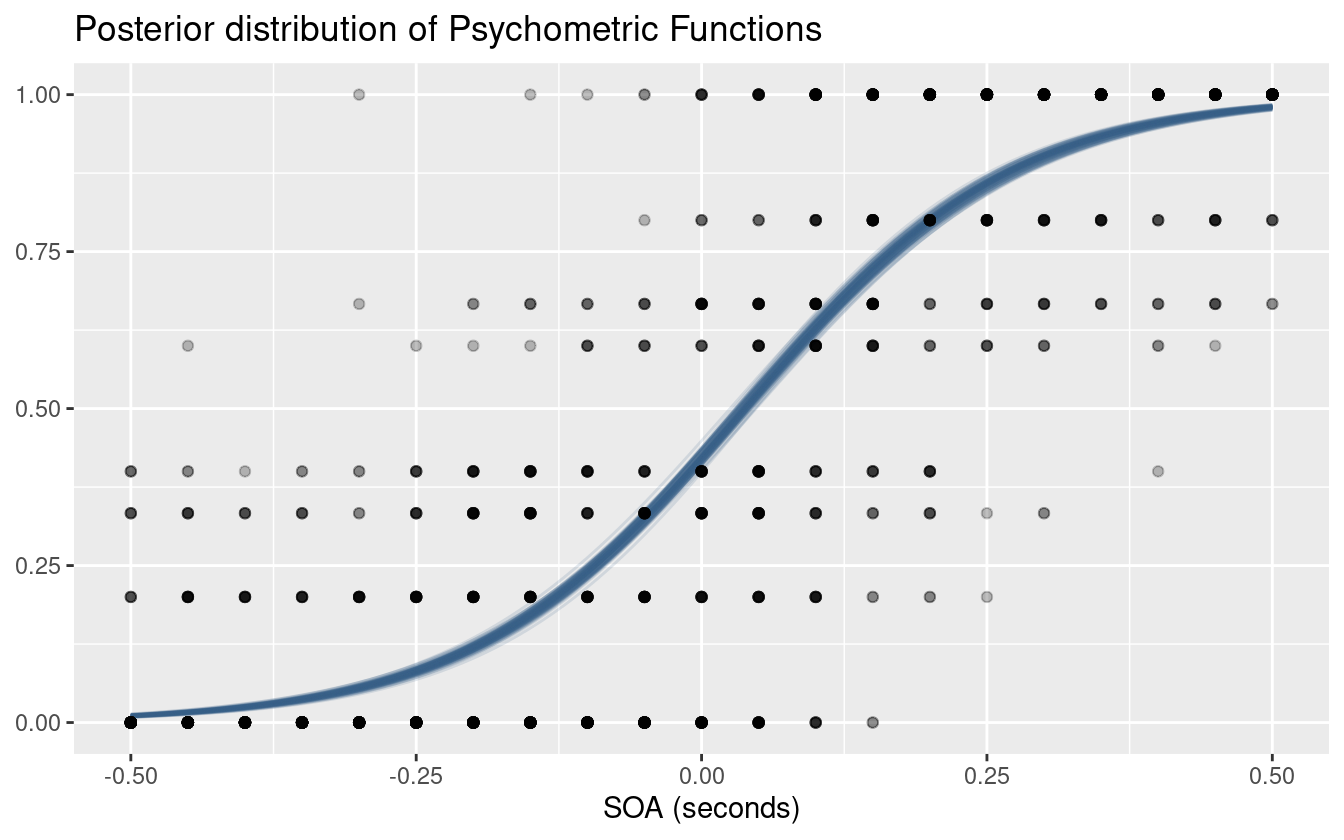
\includegraphics[width=0.85\linewidth]{030-workflow_files/figure-latex/ch031-posterior-pf-plot-1} 

}

\caption{Posterior distribution of psychometric functions using pooled observations.}\label{fig:ch031-posterior-pf-plot}
\end{figure}

Next I sample parameter values from the posterior distribution and use them to simulate a new data set. In the next iteration I will show how I can get Stan to automatically produce retrodictions for me in the model fitting step. The results of the posterior retrodictions are shown in figure \ref{fig:ch031-obs-vs-retro-plot}.

\setstretch{1.0}

\begin{Shaded}
\begin{Highlighting}[]
\NormalTok{alpha <-}\StringTok{ }\KeywordTok{sample}\NormalTok{(p031}\OperatorTok{$}\NormalTok{alpha, n_obs, }\DataTypeTok{replace =} \OtherTok{TRUE}\NormalTok{)}
\NormalTok{beta  <-}\StringTok{ }\KeywordTok{sample}\NormalTok{(p031}\OperatorTok{$}\NormalTok{beta, n_obs, }\DataTypeTok{replace =} \OtherTok{TRUE}\NormalTok{)}
\NormalTok{logodds <-}\StringTok{ }\NormalTok{beta }\OperatorTok{*}\StringTok{ }\NormalTok{(av_dat}\OperatorTok{$}\NormalTok{x }\OperatorTok{-}\StringTok{ }\NormalTok{alpha)}
\NormalTok{probs <-}\StringTok{ }\KeywordTok{logistic}\NormalTok{(logodds)}
\NormalTok{sim_k <-}\StringTok{ }\KeywordTok{rbinom}\NormalTok{(n_obs, av_dat}\OperatorTok{$}\NormalTok{n, probs)}
\end{Highlighting}
\end{Shaded}

\setstretch{2.0}

\begin{figure}

{\centering 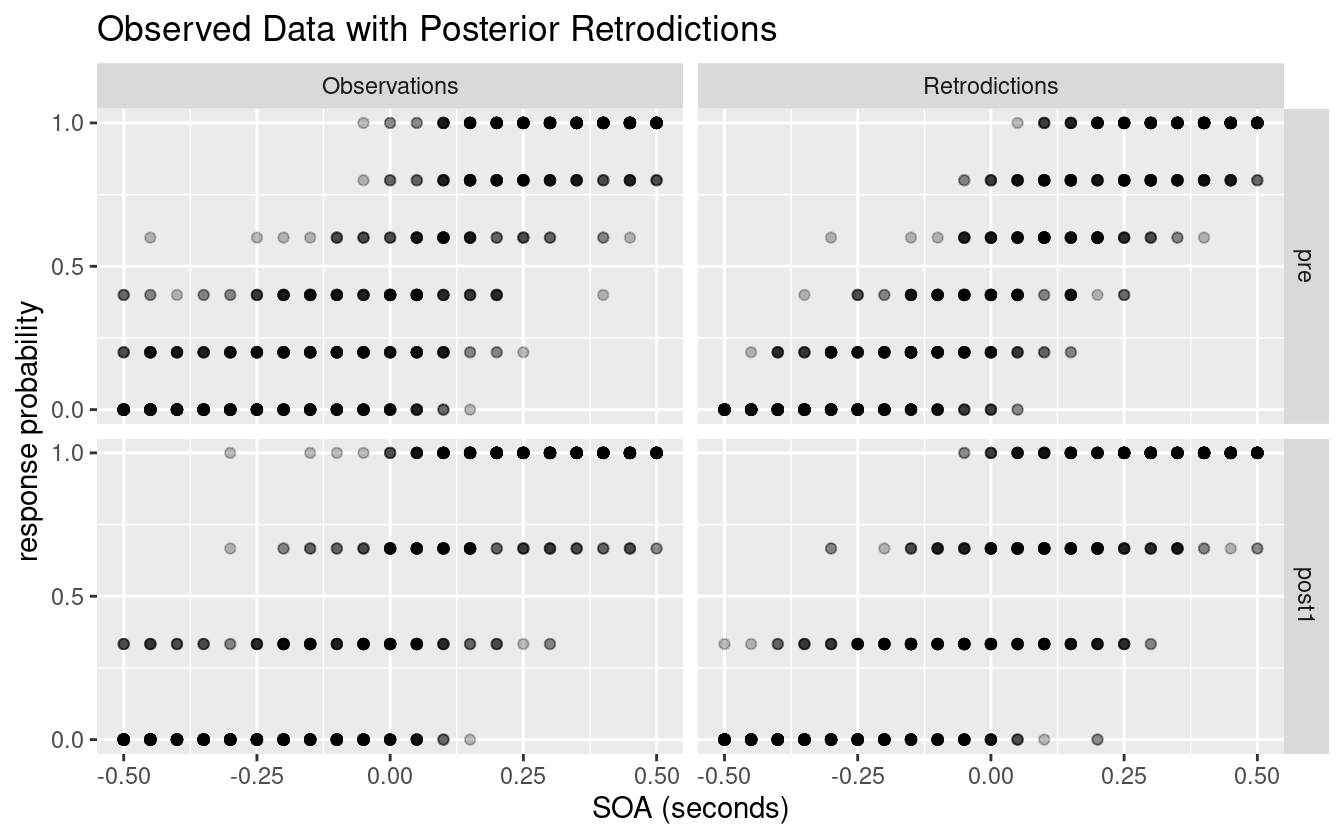
\includegraphics[width=0.85\linewidth]{030-workflow_files/figure-latex/ch031-obs-vs-retro-plot-1} 

}

\caption{Observed data compared to the posterior retrodictions. The data is post-stratified by block for easier visualization.}\label{fig:ch031-obs-vs-retro-plot}
\end{figure}

I want to make it clear exactly what the first iteration of this model tells us. It is the average distribution of underlying psychometric functions across all subjects and blocks. It cannot tell us what the differences are between pre- and post-adaptation blocks are, or even what the variation between subjects is. As such, it is only useful in determining if the average value for the PSS is different from 0 or if the average JND is different from some other predetermined level. This model is still useful given the right question, but this model cannot answer questions about group-level effects.

Figure \ref{fig:ch031-obs-vs-retro-plot} shows that the model captures the broad structure of the observed data, but is perhaps a bit under-dispersed in the tail ends of the SOA values. Besides this one issue, I am satisfied with the first iteration of this model and am ready to proceed to the next iteration.

\hypertarget{iter2}{%
\section{Iteration 2 (electric boogaloo)}\label{iter2}}

In this iteration I will be adding in the treatment and age groups into the model. There are no changes with the conceptual understanding of the experiment, and nothing to change with the observational space. As such I will be skipping the first three steps and go straight to the model development step. As I build the model, the number of changes from one iteration to the next should go to zero as the model \emph{expands} to become only as complex as necessary to answer the research questions.

\textbf{Post-Model, Pre-Data}

\emph{Develop Model}

To start, let's add in the treatment indicator and put off consideration of adding in the age group levels. In classical statistics, it is added as an indicator variable (zero or one) for both the slope and intercept (varying slopes, varying intercepts model). Let \(trt\) be \(0\) if it is the pre-adaptation block and \(1\) if the observation comes from the post-adaptation block.

\setstretch{1.0}

\[
\theta = \alpha + \alpha_{trt} \times trt + \beta \times x + \beta_{trt}\times trt \times x
\]
\setstretch{2.0}

Now when an observation comes from the pre-adaptation block (\(trt=0\)) the linear predictor is given by

\setstretch{1.0}

\[
\theta_{pre} = \alpha + \beta \times x
\]
\setstretch{2.0}

and when an observation comes from the post-adaptation block (\(trt=1\)) the linear predictor is

\setstretch{1.0}

\[
\theta_{post} = (\alpha + \alpha_{trt}) + (\beta + \beta_{trt}) \times x
\]
\setstretch{2.0}

This might seem like a natural way to introduce an indicator variable, but it comes with serious implications. This model implies that there is more uncertainty about the post-adaptation block compared to the baseline block, and this is not necessarily true.

\setstretch{1.0}

\begin{align*}
\mathrm{Var}(\theta_{post}) &= \mathrm{Var}((\alpha + \alpha_{trt}) + (\beta + \beta_{trt}) \times x) \\
&= \mathrm{Var}(\alpha) + \mathrm{Var}(\alpha_{trt}) + x^2 \mathrm{Var}(\beta) + x^2\mathrm{Var}(\beta_{trt})
\end{align*}
\setstretch{2.0}

On the other hand, the variance of \(\theta_{pre}\) is

\setstretch{1.0}

\[
\mathrm{Var}(\theta_{pre}) = \mathrm{Var}(\alpha) + x^2 \mathrm{Var}(\beta) \le \mathrm{Var}(\theta_{post})
\]
\setstretch{2.0}

Furthermore, the intercept, \(\alpha\), is no longer the average response probability at \(x=0\) for the entire data set, but is instead exclusively the average for the pre-adaptation block. This may not matter in certain analyses, but one nice property of multilevel models is the separation of population level estimates and group level estimates (fixed vs.~mixed effects).

So instead the treatment variable is introduced into the linear model as a factor variable. This essentially means that each level in the treatment gets its own parameter estimate, and this also makes it easier to set priors when there are many levels in a group (such as for the subject level). The linear model, using equation \eqref{eq:linearform2}, with the treatment is written as

\setstretch{1.0}

\begin{equation}
  \theta = (\beta + \beta_{trt[i]}) \left[x_i - (\alpha + \alpha_{trt[i]})\right]
  \label{eq:linearmodel2}
\end{equation}
\setstretch{2.0}

As I add in more predictors and groups, equation \eqref{eq:linearmodel2} will start to be more difficult to read. What I can do is break up the slope and intercept parameters and write the linear model as

\setstretch{1.0}

\begin{align*}
\mu_\alpha &= \alpha + \alpha_{trt[i]} \\
\mu_\beta &= \beta + \beta_{trt[i]} \\
\theta &= \mu_\beta (x - \mu_\alpha)
\end{align*}
\setstretch{2.0}

In this way the combined parameters can be considered separately from the linear parameterization. Which leads me to consider the priors for \(\alpha_{trt}\) and \(\beta_{trt}\). The way that we can turn an normal model with categorical predictors into a multilevel model is by allowing the priors to borrow information from other groups. This is accomplished by putting priors on priors. It is easier to write down the model first before explaining how it works.

\setstretch{1.0}

\begin{align*}
k_i &\sim \mathrm{Binomial}(n_i, p_i) \\
\mu_\alpha &= \alpha + \alpha_{trt[i]} \\
\mu_\beta &= \beta + \beta_{trt[i]} \\
\mathrm{logit}(p_i) &= \mu_\beta (x_i - \mu_\alpha) \\
\alpha &\sim \mathcal{N}(0, 0.06^2) \\
\alpha_{trt} &\sim \mathcal{N}(0, \sigma_{trt}^2) \\
\sigma_{trt} &\sim \textrm{to be defined}
\end{align*}
\setstretch{2.0}

In the above model, \(\alpha\) gets a fixed prior (the same as in the first iteration), and \(\alpha_{trt}\) gets a Gaussian prior with an adaptive variance term that is allowed to be learned from the data. This notation is compact, but \(\alpha_{trt}\) is actually two parameters - one each for the pre- and post-adaptation blocks - but they both share the same variance term \(\sigma_{trt}\). This produces a \emph{regularizing} effect where both treatment estimates are shrunk towards the mean, \(\alpha\).

I'll discuss selecting a prior for the variance term shortly, but now I want to discuss setting the prior for the slope terms. Instead of modeling \(\beta\) with a log-normal prior, I can sample from a normal distribution and take the exponential of it to produce a log-normal distribution. I.e.

\setstretch{1.0}

\[
X \sim \mathcal{N}(3, 1^2) \\
Y = \exp\left\lbrace X \right\rbrace \Longleftrightarrow Y \sim \mathrm{Lognormal(3, 1^2)}
\]
\setstretch{2.0}

The motivation behind this transformation is that it is now easier to include new slope variables as an additive affect. If both \(\beta\) and \(\beta_{trt}\) are specified with Gaussian priors, then the exponential of the sum will be a log-normal distribution! So the model now gains

\setstretch{1.0}

\begin{align*}
\mathrm{logit}(p_i) &= \exp(\mu_\beta) (x_i - \mu_\alpha) \\
\beta &\sim \mathcal{N}(3, 1^2) \\
\beta_{trt} &\sim \mathcal{N}(0, \gamma_{trt}^2) \\
\gamma_{trt} &\sim \textrm{to be defined}
\end{align*}
\setstretch{2.0}

Deciding on priors for the variance term requires some careful consideration. In one sense, the variance term is the within group variance. \citet{gelman2006prior} recommends that for multilevel models with groups with less than say 5 levels to use a half Cauchy prior. This weakly informative prior still has a regularizing affect and dissuades larger variance estimates. Even though the treatment group only has two levels, there is still value in specifying an adaptive prior for them, and there is also a lot of data for each treatment so partial pooling won't make a difference anyway.

\setstretch{1.0}

\begin{align*}
\sigma_{trt} &\sim \mathrm{HalfCauchy}(0, 1) \\
\gamma_{trt} &\sim \mathrm{HalfCauchy}(0, 1)
\end{align*}
\setstretch{2.0}

Finally I can add in the age group level effects and specify the variance terms.

\setstretch{1.0}

\begin{align*}
\alpha_{G} &\sim \mathcal{N}(0, \tau_{G}^2)\\
\beta_{G} &\sim \mathcal{N}(0, \nu_{G}^2) \\
\tau_{G} &\sim \mathrm{HalfCauchy}(0, 2) \\
\nu_{G} &\sim \mathrm{HalfCauchy}(0, 2)
\end{align*}
\setstretch{2.0}

The corresponding Stan model is becoming quite long, so I omit it from here on out. The final Stan model code may be found in the \protect\hyperlink{supplementary-code}{supplementary code} of the appendix.

\textbf{Post-Model, Post-Data}

\emph{Fit Observed Data}

I'm choosing to skip the prior checks this time around and use the observed data to configure the algorithm and diagnose the posterior fit.

\setstretch{1.0}

\begin{Shaded}
\begin{Highlighting}[]
\NormalTok{m032 <-}\StringTok{ }\KeywordTok{sampling}\NormalTok{(m032_stan, }\DataTypeTok{data =}\NormalTok{ obs_dat, }\DataTypeTok{seed =} \DecValTok{124}\NormalTok{,}
                 \DataTypeTok{chains =} \DecValTok{4}\NormalTok{, }\DataTypeTok{cores =} \DecValTok{4}\NormalTok{, }\DataTypeTok{refresh =} \DecValTok{100}\NormalTok{)}
\end{Highlighting}
\end{Shaded}

\setstretch{2.0}

\emph{Diagnose Posterior Fit}

\setstretch{1.0}

\begin{Shaded}
\begin{Highlighting}[]
\KeywordTok{check_hmc_diagnostics}\NormalTok{(m032)}
\CommentTok{#> }
\CommentTok{#> Divergences:}
\CommentTok{#> 4 of 4000 iterations ended with a divergence (0.1%).}
\CommentTok{#> Try increasing 'adapt_delta' to remove the divergences.}
\CommentTok{#> }
\CommentTok{#> Tree depth:}
\CommentTok{#> 0 of 4000 iterations saturated the maximum tree depth of 10.}
\CommentTok{#> }
\CommentTok{#> Energy:}
\CommentTok{#> E-BFMI indicated no pathological behavior.}
\end{Highlighting}
\end{Shaded}

\setstretch{2.0}

As well as the 4 divergent transitions, there was also a message about the effective sample size (ESS) being too low. The recommended prescription for low ESS is to run the chains for more iterations. The posterior summary shows that \(N_{\mathrm{eff}}\) is low for the age group level parameters (table \ref{tab:ch032-Liquid-Strawberry-Eagle}).

\begin{table}[!h]

\caption{\label{tab:ch032-Liquid-Strawberry-Eagle}Summary statistics of the second iteration.}
\centering
\begin{tabular}[t]{lrrrrrrr}
\toprule
parameter & mean & se\_mean & sd & 2.5\% & 97.5\% & n\_eff & Rhat\\
\midrule
a & 0.0222 & 0.0014 & 0.0412 & -0.0683 & 0.1024 & 824.6 & 1.002\\
aG[1] & -0.0009 & 0.0012 & 0.0313 & -0.0531 & 0.0714 & 703.5 & 1.003\\
aG[2] & 0.0274 & 0.0012 & 0.0316 & -0.0218 & 0.0990 & 698.3 & 1.003\\
aG[3] & -0.0078 & 0.0012 & 0.0311 & -0.0609 & 0.0609 & 714.3 & 1.004\\
b & 2.4114 & 0.0216 & 0.5665 & 1.4902 & 3.8499 & 688.2 & 1.003\\
\addlinespace
bG[1] & 0.0030 & 0.0170 & 0.2942 & -0.7681 & 0.5013 & 301.3 & 1.004\\
bG[2] & 0.0538 & 0.0170 & 0.2940 & -0.7101 & 0.5499 & 299.9 & 1.004\\
bG[3] & -0.2223 & 0.0172 & 0.2955 & -1.0150 & 0.2597 & 296.9 & 1.004\\
\bottomrule
\end{tabular}
\end{table}

So I can go back to the algorithm configuration step and increase the number of iterations and warm-up iterations, as well as increase the adapt delta parameter to reduce the number of divergent transitions (which really isn't a problem right now).

Another technique I can employ is non-centered parameterization, and now is as good a time as any to introduce it. I have actually already used non-centered parameterization in this iteration of the model without addressing it - the transformation of \(\beta\) from a Gaussian to a log-normal distribution.

Because HMC is a physics simulation, complicated geometry or posteriors with steep slopes can be difficult to traverse if the step size is too course. The solution is to explore a simpler geometry, and then transform the sample into the target distribution. Reparameterization is especially important for hierarchical models. The Cauchy distribution used for the variance term can be reparameterized by first drawing from a uniform distribution on \((-\pi/2, \pi/2)\). For a half Cauchy distribution, just sample from \(\mathcal{U}(0, \pi/2)\).

\setstretch{1.0}

\begin{align*}
X &\sim \mathcal{U}(-\pi/2, \pi/2) \\
Y &= \mu + \tau \cdot \tan(X) \Longrightarrow Y \sim \mathrm{Cauchy(\mu, \tau)}
\end{align*}
\setstretch{2.0}

The Gaussian distributions can be reparameterized in a similar way. If \(Z\) is a standard normal random variable, then \(\mu + \sigma Z \sim \mathcal{N}(\mu, \sigma^2)\). For Stan, sampling from a standard normal or uniform distribution is very easy, and so the non-centered parameterization can alleviate divergent transitions. I now return to the model development step and incorporate the new methods.

\emph{Develop Model}

The model changes consist of using the non-centered parameterizations discussed in the previous step. An example is in the parameterization of \(\tau_{G}\). The other variance terms are parameterized in the same fashion.

\setstretch{1.0}

\begin{align*}
U_\tau &\sim \mathcal{U}(0, \pi/2) \\
\tau_{G} &= 2 \cdot \tan(U_1) \Longrightarrow \tau_G \sim \mathrm{HalfCauchy}(0, 2)
\end{align*}
\setstretch{2.0}

As an aside, a multilevel model can be fit in R using \texttt{lme4::glmer}, \texttt{brms::brm}, or \texttt{rstanarm::stan\_glmer}, and they all use the same notation to specify the model. The notation is very compact, but easy to unpack. Values not in a grouping term are \emph{fixed} effects and values in a grouping term (e.g.~\texttt{(1\ +\ x\ \textbar{}\ G)}) are \emph{mixed} or \emph{random} effects depending on which textbook you read.

\setstretch{1.0}

\begin{Shaded}
\begin{Highlighting}[]
\NormalTok{f <-}\StringTok{ }\KeywordTok{formula}\NormalTok{(k}\OperatorTok{|}\NormalTok{n }\OperatorTok{~}\StringTok{ }\DecValTok{1} \OperatorTok{+}\StringTok{ }\NormalTok{x }\OperatorTok{+}\StringTok{ }\NormalTok{(}\DecValTok{1} \OperatorTok{+}\StringTok{ }\NormalTok{x }\OperatorTok{|}\StringTok{ }\NormalTok{G) }\OperatorTok{+}\StringTok{ }\NormalTok{(}\DecValTok{1} \OperatorTok{+}\StringTok{ }\NormalTok{x }\OperatorTok{|}\StringTok{ }\NormalTok{trt))}

\NormalTok{lme4}\OperatorTok{::}\KeywordTok{glmer}\NormalTok{(f, }\DataTypeTok{data =}\NormalTok{ data, }\DataTypeTok{family =} \KeywordTok{binomial}\NormalTok{(}\StringTok{"logit"}\NormalTok{))}
\NormalTok{rstanarm}\OperatorTok{::}\KeywordTok{stan_glmer}\NormalTok{(f, }\DataTypeTok{data =}\NormalTok{ data, }\DataTypeTok{family =} \KeywordTok{binomial}\NormalTok{(}\StringTok{"logit"}\NormalTok{))}
\NormalTok{brms}\OperatorTok{::}\KeywordTok{brm}\NormalTok{(f, }\DataTypeTok{data =}\NormalTok{ data, }\DataTypeTok{family =} \KeywordTok{binomial}\NormalTok{(}\StringTok{"logit"}\NormalTok{))}
\end{Highlighting}
\end{Shaded}

\setstretch{2.0}

The simpler notation and compactness of these methods are very attractive, and for certain analyses they may be more than sufficient. The goal here is to decide early on if these methods satisfy the model adequacy, and to use more flexible modeling tools like Stan if necessary.

\emph{Fit Observed Data}

Moving on to refitting the data, this time with more iterations and with the non-centered parameterization. Since this model is sampling from intermediate parameters, I can choose to keep only the transformed parameters.

\setstretch{1.0}

\begin{Shaded}
\begin{Highlighting}[]
\NormalTok{m032nc <-}\StringTok{ }\KeywordTok{sampling}\NormalTok{(m032nc_stan, }\DataTypeTok{data =}\NormalTok{ obs_dat, }\DataTypeTok{seed =} \DecValTok{143}\NormalTok{,}
                   \DataTypeTok{iter =} \DecValTok{4000}\NormalTok{, }\DataTypeTok{warmup =} \DecValTok{2000}\NormalTok{, }\DataTypeTok{pars =}\NormalTok{ keep_pars,}
                   \DataTypeTok{control =} \KeywordTok{list}\NormalTok{(}\DataTypeTok{adapt_delta =} \FloatTok{0.95}\NormalTok{), }\DataTypeTok{thin =} \DecValTok{2}\NormalTok{,}
                   \DataTypeTok{chains =} \DecValTok{4}\NormalTok{, }\DataTypeTok{cores =} \DecValTok{4}\NormalTok{, }\DataTypeTok{refresh =} \DecValTok{100}\NormalTok{)}
\end{Highlighting}
\end{Shaded}

\setstretch{2.0}

\emph{Diagnose Posterior Fit}

\setstretch{1.0}

\begin{Shaded}
\begin{Highlighting}[]
\KeywordTok{check_hmc_diagnostics}\NormalTok{(m032nc)}
\CommentTok{#> }
\CommentTok{#> Divergences:}
\CommentTok{#> 32 of 4000 iterations ended with a divergence (0.8%).}
\CommentTok{#> Try increasing 'adapt_delta' to remove the divergences.}
\CommentTok{#> }
\CommentTok{#> Tree depth:}
\CommentTok{#> 0 of 4000 iterations saturated the maximum tree depth of 10.}
\CommentTok{#> }
\CommentTok{#> Energy:}
\CommentTok{#> E-BFMI indicated no pathological behavior.}
\end{Highlighting}
\end{Shaded}

\setstretch{2.0}

There are still a few divergent transitions (\(<1\%\)), but the effective sample size increased significantly (table \ref{tab:ch032-Bleeding-Tuna}).

\begin{table}[!h]

\caption{\label{tab:ch032-Bleeding-Tuna}Summary statistics of the second iteration with non-centered parameterization.}
\centering
\begin{tabular}[t]{lrrrrrrr}
\toprule
parameter & mean & se\_mean & sd & 2.5\% & 97.5\% & n\_eff & Rhat\\
\midrule
a & 0.0192 & 0.0008 & 0.0419 & -0.0744 & 0.0956 & 2509 & 1.0005\\
aG[1] & -0.0025 & 0.0006 & 0.0326 & -0.0636 & 0.0739 & 2737 & 1.0014\\
aG[2] & 0.0262 & 0.0006 & 0.0328 & -0.0342 & 0.1044 & 2644 & 1.0014\\
aG[3] & -0.0093 & 0.0006 & 0.0326 & -0.0713 & 0.0652 & 2752 & 1.0011\\
aT[1] & 0.0185 & 0.0009 & 0.0425 & -0.0546 & 0.1242 & 2338 & 1.0005\\
\addlinespace
aT[2] & 0.0039 & 0.0009 & 0.0419 & -0.0679 & 0.1089 & 2404 & 1.0005\\
b & 2.3841 & 0.0115 & 0.5284 & 1.4762 & 3.6952 & 2109 & 1.0010\\
bG[1] & 0.0170 & 0.0049 & 0.2730 & -0.6323 & 0.4979 & 3106 & 1.0004\\
bG[2] & 0.0678 & 0.0049 & 0.2728 & -0.5773 & 0.5671 & 3113 & 1.0005\\
bG[3] & -0.2075 & 0.0050 & 0.2741 & -0.8506 & 0.2767 & 3026 & 1.0004\\
\addlinespace
bT[1] & -0.2764 & 0.0106 & 0.4914 & -1.6338 & 0.5427 & 2141 & 0.9999\\
bT[2] & -0.0501 & 0.0106 & 0.4909 & -1.4120 & 0.7778 & 2125 & 1.0000\\
\bottomrule
\end{tabular}
\end{table}

Now is also a good time to introduce a diagnostic tool called the \emph{trace plot}. The trace plot is a way to visualize the sampling path of different parameters across all the chains. A healthy set of chains will look like a fuzzy caterpillar, bouncing around the posterior without any visual patterns or long sequences of being in the same place. Figure \ref{fig:ch032-traceplot-m032nc} shows the trace plot for the slope and intercept parameters. Each chain looks like it is sampling around the same average value as the others with identical spreads (stationary and homoscedastic). This also helps to solidify the idea that the \(\hat{R}\) statistic is the measure of between chain variance compared to cross chain variance.

\begin{figure}

{\centering \includegraphics[width=0.85\linewidth]{030-workflow_files/figure-latex/ch032-traceplot-m032nc-1} 

}

\caption{Traceplot for the slope and intercept parameters.}\label{fig:ch032-traceplot-m032nc}
\end{figure}

The chains in figure \ref{fig:ch032-traceplot-m032nc} look healthy as well as for the other parameters not shown. Since there are no algorithm issues, I can proceed to the posterior retrodictive checks.

\emph{Posterior Retrodictive Checks}

In this iteration of the model, I now have estimates for the age groups and the treatment. The posterior estimates for the PSS and JND are shown in figure \ref{fig:ch032-posterior-pss-jnd-plot}. There are many ways to visualize and compare the distributions across age groups and conditions, and it really depends on what question is being asked. If for example the question is ``what is the qualitative difference between pre- and post-adaptation across age groups?'', then figure \ref{fig:ch032-posterior-pss-jnd-plot} could answer that because it juxtaposes the two blocks in the same panel. I will consider alternative ways of arranging the plots in \protect\hyperlink{results}{chapter 5}.

\begin{figure}

{\centering \includegraphics[width=0.85\linewidth]{030-workflow_files/figure-latex/ch032-posterior-pss-jnd-plot-1} 

}

\caption{Posterior distribution of the PSS and JND.}\label{fig:ch032-posterior-pss-jnd-plot}
\end{figure}

As for the posterior retrodictions, I can do something similar to last time. First I'd like to point out that I had Stan perform posterior retrodictions during the fitting step. This was achieved by adding a \emph{generated quantities} block to the Stan program that takes the posterior samples for the parameters, and then randomly generates a value from a binomial distribution for each observation in the data. In effect, I now have \(4000\) simulated data sets!

I only need one to compare to the observed data, so I will select it randomly from the posterior.

\begin{figure}

{\centering 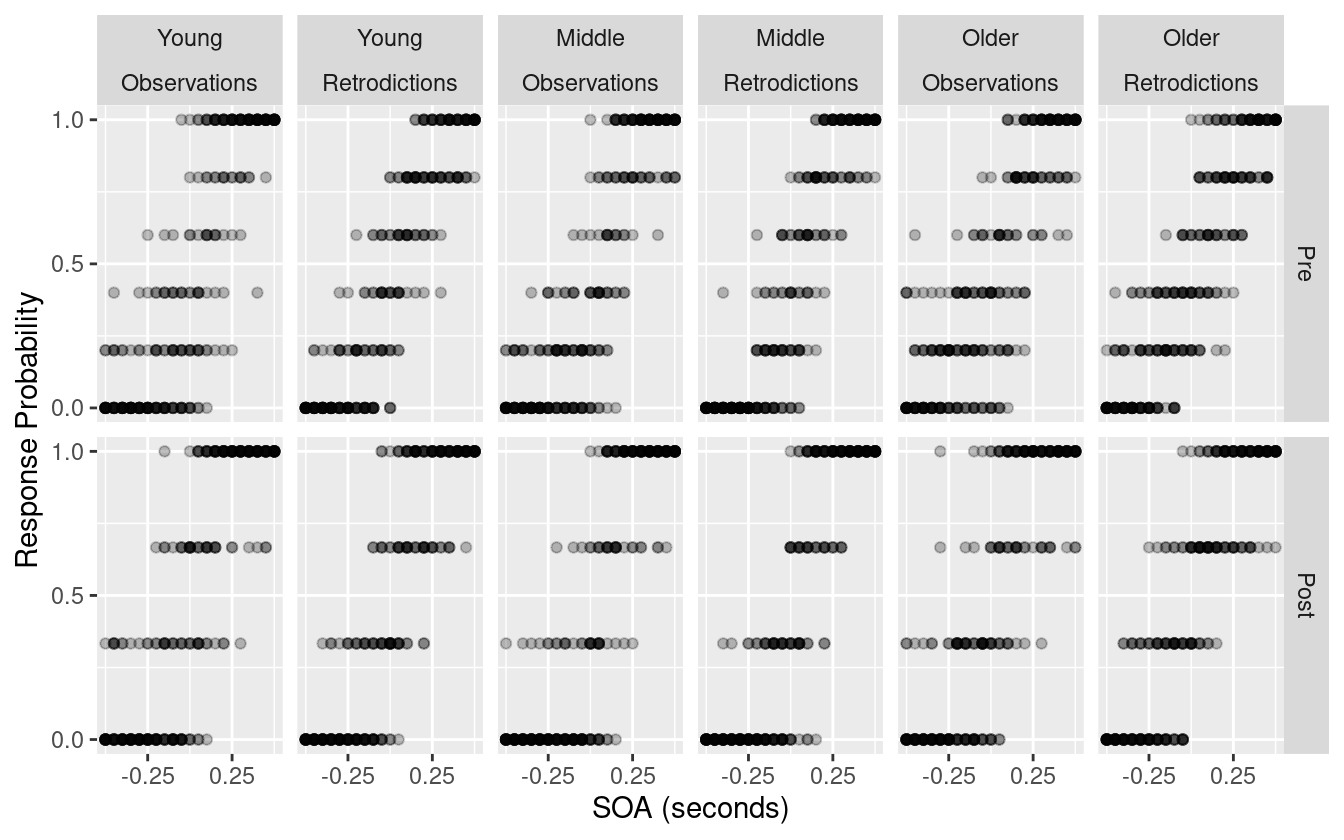
\includegraphics[width=0.85\linewidth]{030-workflow_files/figure-latex/ch032-obs-vs-retro-plot-1} 

}

\caption{Observed data compared to the posterior retrodictions.}\label{fig:ch032-obs-vs-retro-plot}
\end{figure}

The posterior retrodictions in figure \ref{fig:ch032-obs-vs-retro-plot} show no disagreement between the model and the observed data. I almost would say that this model is complete, but this model has one more problem - it measures the average difference in blocks, and the average difference in age groups, but does not consider any interaction between the two! Implicitly it assumes that temporal recalibration affects all age groups the same which may not be true, so in the next iteration I will need to address that.

\hypertarget{iter3}{%
\section{Iteration 3 (the one for me)}\label{iter3}}

Since there is no change in the pre-model analysis, I'll again jump straight to the model development step, after which I will jump right to the posterior retrodictive checks. The changes to the model going forward are minor, and subsequent steps are mostly repetitions of the ones taken in the first two iterations.

\emph{Develop Model}

This time around I need to model an interaction between age group and treatment. In a simple model in R, interactions between factor variable \(A\) and factor variable \(B\) can be accomplished by taking the cross-product of all the factor levels. For example, if \(A\) has levels \(a, b, c\) and \(B\) has levels \(x, y\), then the interaction variable \(C=A:B\) will have levels \(ax, ay, bx, by, cx, cy\). The concept is similar in Stan - create a new variable that is indexed by the cross of the two other factor variables.

\setstretch{1.0}

\[
\beta_{G[i] \times trt[i]} \Longrightarrow bGT[G[i], trt[i]] 
\]
\setstretch{2.0}

In the above expression, the interaction variable \(\beta_{G[i] \times trt[i]}\) is between age group and treatment. The right hand side is the corresponding Stan parameter. Notice that it is an array-like object that is indexed by the age group at observation \(i\) and the treatment at observation \(i\). For example, observation \(51\) is from a middle age adult subject during the post-adaptation block, so \(bGT[G[51], trt[51]] = bGT[2, 2]\). An interaction term is added for both the slope and intercept in this iteration.

\textbf{Post-Model, Post-Data}

\emph{Posterior Retrodictive Checks}

Again, I'll start with the PSS and JND posterior densities. Because the model now allows for the interaction of age group and block, there is no longer a fixed shift in the posterior distribution of the PSS and JND values. Figure \ref{fig:ch033-posterior-pss-jnd-plot} shows that temporal recalibration had no discernible affect on the PSS estimates for the middle age group.

\begin{figure}

{\centering \includegraphics[width=0.85\linewidth]{030-workflow_files/figure-latex/ch033-posterior-pss-jnd-plot-1} 

}

\caption{Posterior distribution of the PSS and JND.}\label{fig:ch033-posterior-pss-jnd-plot}
\end{figure}

The posterior retrodictions for this model are going to be similar to the last iteration. Instead, I want to see how this model performs when it comes to the posterior retrodictions of the visual TOJ data. There is something peculiar about that data that is readily apparent when I try to fit a GLM using classical MLE.

\setstretch{1.0}

\begin{Shaded}
\begin{Highlighting}[]
\NormalTok{vis_mle <-}\StringTok{ }\KeywordTok{glm}\NormalTok{(}\KeywordTok{cbind}\NormalTok{(k, n}\OperatorTok{-}\NormalTok{k) }\OperatorTok{~}\StringTok{ }\DecValTok{0} \OperatorTok{+}\StringTok{ }\NormalTok{sid }\OperatorTok{+}\StringTok{ }\NormalTok{sid}\OperatorTok{:}\NormalTok{soa,}
               \DataTypeTok{data =}\NormalTok{ visual_binomial, }\DataTypeTok{family =} \KeywordTok{binomial}\NormalTok{(}\StringTok{"logit"}\NormalTok{))}
\end{Highlighting}
\end{Shaded}

\setstretch{2.0}

I get a message saying that the fitted probabilities are numerically 0 or 1. What does this mean? First this model estimates a slope and an intercept for each subject individually (no pooling model), so we can look at the estimates for each subject. Table \ref{tab:ch033-Intensive-Oyster} shows the top 3 coefficients sorted by largest standard error of the estimate for both slope and intercept.

\begin{table}[!h]

\caption{\label{tab:ch033-Intensive-Oyster}Coefficients with the largest standard errors.}
\centering
\begin{tabular}[t]{llrrrr}
\toprule
Subject & Coefficient & Estimate & Std. Error & z value & Pr(>|z|)\\
\midrule
O-f-MW & Intercept & -3.6313 & 1.2170 & -2.9837 & 0.0028\\
M-f-CC & Intercept & -2.4925 & 1.0175 & -2.4497 & 0.0143\\
M-f-DB & Intercept & -1.0928 & 0.6389 & -1.7105 & 0.0872\\
Y-m-CB & Slope & 0.6254 & 12.7380 & 0.0491 & 0.9608\\
M-f-DB & Slope & 0.1434 & 0.0442 & 3.2471 & 0.0012\\
\addlinespace
M-f-CC & Slope & 0.1434 & 0.0442 & 3.2471 & 0.0012\\
\bottomrule
\end{tabular}
\end{table}

The standard error of the slope estimate for subject \texttt{Y-m-CB} is incredibly large in comparison to its own estimate and in comparison to the slope with the next largest standard error. To see what's going wrong, let's look at the graph for this subject.

\begin{figure}

{\centering \includegraphics[width=0.85\linewidth]{030-workflow_files/figure-latex/ch033-Y-m-CB-vis-response-1} 

}

\caption{There is almost complete separation in the data.}\label{fig:ch033-Y-m-CB-vis-response}
\end{figure}

Figure \ref{fig:ch033-Y-m-CB-vis-response} shows that there is almost perfect separation in the data for this subject, and that is giving the MLE algorithm trouble. It also has serious consequences on the estimated JND as the estimated JND for this subject is just 3ms which is suspect.

Of course one remedy for this is to pool observations together as I have done for the model in this iteration. The data is pooled together at the age group level and variation in the subjects' responses removes the separation. This isn't always ideal, as sometimes we may be interested in studying the individuals within the experiment. If we can't get accurate inferences about the individual, then the results are not valid. The better solution is to use a hierarchical model! With a hierarchical model, individual estimates are shrunk towards the group mean, and so inferences about individuals may be made along with inferences about the group that contains them. I am interested only in the group level inferences right now, but in \protect\hyperlink{predictive-inference}{chapter 5} I will compare the group level model at the end of this chapter to a model that includes individual estimates.

Figure \ref{fig:ch033-Iron-Intensive} shows the posterior distribution of psychometric functions for the visual TOJ data. Notice that there is almost no difference between the pre- and post-adaptation blocks.

\begin{figure}

{\centering \includegraphics[width=0.85\linewidth]{figures/ch033-Iron-Intensive} 

}

\caption{Posterior distribution of psychometric functions for the visual TOJ data. There is almost no visual difference between the pre- and post-adaptation blocks.}\label{fig:ch033-Iron-Intensive}
\end{figure}

Furthermore, as shown by the posterior retrodictions (figure \ref{fig:ch033-obs-vs-retro-plot}), the model is not fully capturing the variation in the responses near the outer SOA values. I.e. the posterior retrodictions are tight around SOA values near zero.

\begin{figure}

{\centering 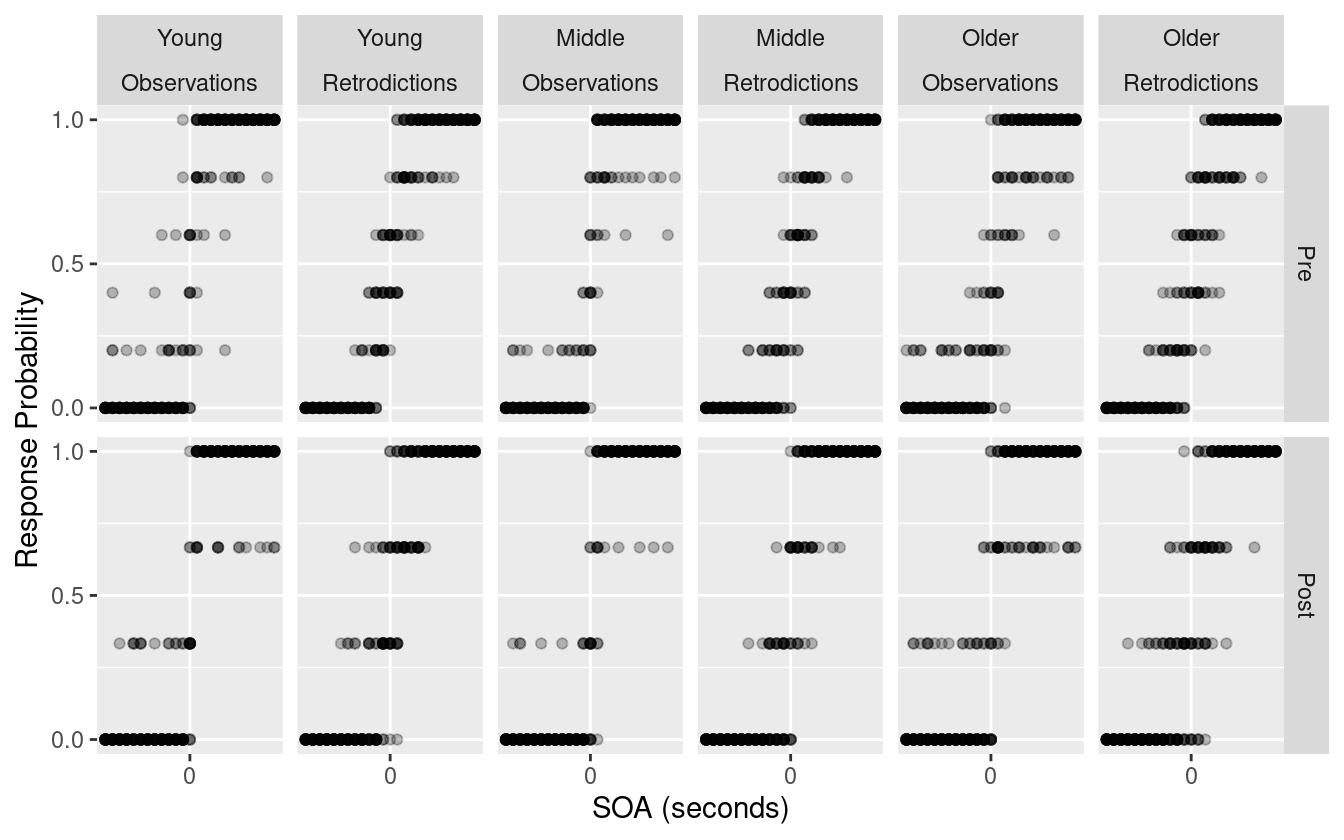
\includegraphics[width=0.85\linewidth]{030-workflow_files/figure-latex/ch033-obs-vs-retro-plot-1} 

}

\caption{Observed visual TOJ data compared to the posterior retrodictions. The retrodictions are not capturing the variation at the outer SOA values.}\label{fig:ch033-obs-vs-retro-plot}
\end{figure}

So why is the model having difficulty expressing the data? Well as it turns out, there is one more concept pertaining to psychometric experiments that I have left out until now, and that is a lapse in judgment. Not a lapse in judgment on my part, but the actual act of having a lapse while performing an experiment. So now, dear reader, I hope you have it in you for one last iteration of this model before moving on to read about the long sought after results.

\hypertarget{iter4}{%
\section{Iteration 4 (what's one more)}\label{iter4}}

\textbf{Pre-Model, Pre-Data}

\emph{Conceptual Analysis}

A lapse in judgment can happen for any reason, and is assumed to be random and independent of other lapses. They can come in the form of the subject accidentally blinking during the presentation of a visual stimulus, or unintentionally pressing the wrong button to respond. Whatever the case is, lapses can have a significant affect on estimating the psychometric function.

\textbf{Post-Model, Pre-Data}

\emph{Develop Model}

Lapses can be modeled as occurring independently at some fixed rate. Fundamentally this means that the underlying performance function, \(F\), is bounded by some lower and upper lapse rate. This manifests as a scaling and translation of \(F\). For a given lower and upper lapse rate \(\lambda\) and \(\gamma\), the performance function \(\Psi\) is

\setstretch{1.0}

\[
\Psi(x; \alpha, \beta, \lambda, \gamma) = \lambda + (1 - \lambda - \gamma) F(x; \alpha, \beta)
\]
\setstretch{2.0}

\begin{figure}

{\centering \includegraphics[width=0.85\linewidth]{030-workflow_files/figure-latex/ch034-plot-pf-with-lapse-1} 

}

\caption{Psychometric function with lower and upper performance bounds.}\label{fig:ch034-plot-pf-with-lapse}
\end{figure}

In certain psychometric experiments, \(\lambda\) is interpreted as the lower performance bound or the guessing rate. For example, in certain 2-alternative forced choice (2-AFC) tasks, subjects are asked to respond which of two masses is heavier, and the correctness of their response is recorded. When the masses are the same, the subject can do no better than random guessing. In this task, the lower performance bound is assumed to be 50\% as their guess is split between two choices. As the absolute difference in mass grows, the subject's correctness rate increases, though lapses can still happen. In this scenario, \(\lambda\) is fixed at \(0.5\) and the lapse rate \(\gamma\) is a parameter in the model.

The model I am building for this data does not explicitly record correctness, so I do not give \(\lambda\) the interpretation of a guessing rate. Since the data are recorded as proportion of positive responses, I instead treat \(\lambda\) and \(\gamma\) as lapse rates for negative and positive SOAs. But why should the upper and lower lapse rates be treated separately? A lapse in judgment can occur independently of the SOA, so \(\lambda\) and \(\gamma\) should be the same no matter what. With this assumption in mind, I can throw away \(\gamma\) and assume that the lower and upper performance bounds are restricted by the same amount. I.e.

\setstretch{1.0}

\begin{equation}
  \Psi(x; \alpha, \beta, \lambda) = \lambda + (1 - 2\lambda) F(x; \alpha, \beta)
  \label{eq:Psi}
\end{equation}
\setstretch{2.0}

While I'm throwing in a lapse rate, I'll also ask the question if different age groups have different lapse rates. To answer this (or rather have the model answer this), I include the new parameter \(\lambda_{G[i]}\) into the model so that the lapse rate is estimated for each age group.

It's okay to assume that lapses in judgment are rare, and it's also true that the rate (or probability) of a lapse is bounded in the interval \([0, 1]\). Because of this, I put a \(\mathrm{Beta(4, 96)}\) prior on \(\lambda\) which \emph{a priori} puts 99\% of the weight below \(0.1\) and an expected lapse rate of \(0.04\).

I could also set up the model so that information about the lapse rate is shared between age groups (i.e.~multilevel), but I'll leave that as an exercise for the reader.

\emph{Construct Summary Functions}

Since the fundamental structure of the linear model has changed, it is worth updating the summary function that computes the distribution of SOA values for a given response probability. Given equation \eqref{eq:Psi}, the summary function \(Q\) is

\setstretch{1.0}

\[
Q(\pi; \alpha, \beta, \lambda) = F_{\alpha, \beta}^{-1}\left(\frac{\pi - \lambda}{1 - 2\lambda}\right) = \frac{1}{\exp(\beta)} \cdot \mathrm{logit}\left(\frac{\pi - \lambda}{1-2\lambda}\right) + \alpha
\]
\setstretch{2.0}

\textbf{Post-Model, Post-Data}

\emph{Fit Observed Data}

Because it is the visual data that motivated this iteration, I will finish up using that data to fit the model and perform posterior retrodictive checks.

\emph{Posterior Retrodictive Checks}

The plot for the distribution of psychometric functions is repeated one more time below (figure \ref{fig:ch034-Screaming-Proton}). There is now visual separation between the pre- and post-adaptation blocks, with the latter exhibiting a higher slope, which in turn implies a reduced just noticeable difference which is consistent with the audiovisual data in the previous model.

\begin{figure}

{\centering \includegraphics[width=0.85\linewidth]{figures/ch034-Screaming-Proton} 

}

\caption{There is now a visual distinction between the two blocks unlike in the model without lapse rate. The lapse rate acts as a balance between steep slopes near the PSS and variation near the outer SOA values.}\label{fig:ch034-Screaming-Proton}
\end{figure}

As for the posterior retrodictions, the model is now better capturing the outer SOA variation. This can best be seen in the comparison of the younger adult pre-adaptation block of figure \ref{fig:ch034-Insane-Metaphor}.

\begin{figure}

{\centering 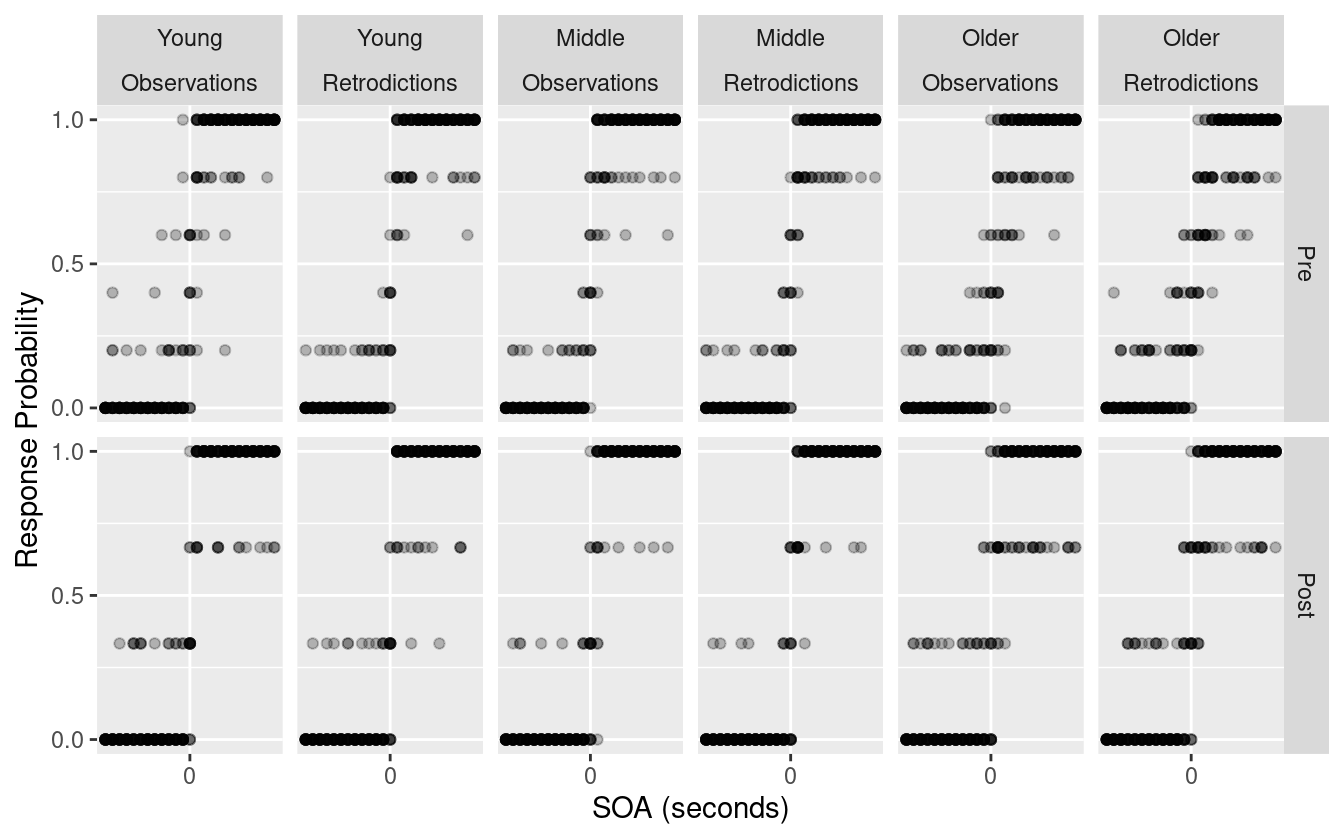
\includegraphics[width=0.85\linewidth]{030-workflow_files/figure-latex/ch034-Insane-Metaphor-1} 

}

\caption{The lapse rate produces posterior retrodictions that are visually more similar to the observed data than in the previous model, suggesting that the model is now just complex enough to capture the relevant details of the data generating process.}\label{fig:ch034-Insane-Metaphor}
\end{figure}

\hypertarget{celebrate}{%
\section{Celebrate}\label{celebrate}}

\emph{celebrate}

\hypertarget{model-checking}{%
\chapter{Model Fitting/Checking}\label{model-checking}}

\emph{Check your model before you wreck your model}

This chapter serves as the formal home of definitions and explanations of concepts relating to Markov Chain Monte Carlo (MCMC) and other diagnostic tools when working with Bayesian inference models. I touched on the physics of Hamiltonian Monte Carlo (HMC) and the diagnostic tools that come with it in the previous chapter, but now I will go into more detail.

\hypertarget{fitting-using-hmc}{%
\section{Fitting using HMC}\label{fitting-using-hmc}}

Why do we need a sampler at all? Bayesian statistics and modeling stems from Bayes theorem (Equation \eqref{eq:bayesthm}). The prior \(P(\theta)\) is some distribution over the parameter space and the likelihood \(P(X | \theta)\) is the probability of an outcome in the sample space given a value in the parameter space. To keep things simple, we generally say that the posterior is proportional to the prior times the likelihood. Why proportional? The posterior distribution is a probability distribution, which means that the sum or integral over the parameter space must evaluate to one. Because of this constraint, the denominator in \eqref{eq:bayesthm} acts as a scale factor to ensure that the posterior is valid.

\begin{equation}
  P(\theta | X) = \frac{P(X | \theta)\cdot P(\theta)}{\sum_i P(X | \theta_i)} =   \frac{P(X | \theta)\cdot P(\theta)}{\int_\Omega P(X | \theta)d\theta}
  \label{eq:bayesthm}
\end{equation}

For simple models, the posterior distribution can sometimes be evaluated analytically. An example of this is in \emph{conjugate} models, where the resulting posterior distribution is of the same type as the prior distribution, and an example of a conjugate model is the Beta distribution for inference about a proportion statistic. This is common in baseball for a player's batting average. I don't know a lot about baseball, but I know that hitting a baseball is a little less common than one in three swings, so \emph{a priori} I believe the probability of hitting a baseball is distributed as \(\mathrm{Beta}(2, 5)\) because the expected value is \(\approx 0.29\) and not a lot of weight is given to any particular value. Throughout a game I follow one player and he hits four balls and misses six - data that can be modeled as a Binomial observation. To figure out the posterior distribution for batting average, I use Bayes' theorem - \emph{posterior is proportional to the prior times the likelihood}.

\begin{align*}
  P(\pi | y) &\propto P(y | \pi) \cdot P(\pi) \\
  &= {10 \choose 4}\pi^{4} (1-\pi)^{6} \cdot \frac{\Gamma(2+5)}{\Gamma(2)\Gamma(5)} \pi^{2-1}(1-\pi)^{5-1} \\
  &\propto \pi^{4+2-1}(1-\pi)^{6+5-1} \\
  &= \pi^{6-1}(1-\pi)^{11-1}
\end{align*}

The final line is the shape of a Beta distribution with parameters \(6=2+4\) and \(11=5+6\). The simple update rule is that for a prior \(\mathrm{Beta}(a, b)\) and observed data with \(y\) successes in \(n\) observations, the posterior distribution is \(\mathrm{Beta}(a + y, b + n - y)\). For the baseball player, the Bayesian estimate of his batting average is \(6/(6+11) \approx 0.353\), but still with a good amount of uncertainty as shown in figure \ref{fig:ch040-Teal-Monkey}.

\begin{figure}

{\centering \includegraphics[width=0.85\linewidth]{040-model-checking_files/figure-latex/ch040-Teal-Monkey-1} 

}

\caption{After observing 4 hits in 10, the Beta(2,5) prior gets updated to become a Beta(6,11) posterior.}\label{fig:ch040-Teal-Monkey}
\end{figure}

Conjugate models are great for simple observational data, but often it happens that the posterior distribution cannot be deduced from the model or that the integral in the denominator is complex or of a high dimension. In the former situation, the integral may not be possible to evaluate, and in the latter there may not be enough computational resources in the world to perform a simple grid approximation.

The solution is to use Markov Chain Monte Carlo (MCMC). The idea is that we can \emph{draw samples} from the posterior distribution in a way that samples proportional to the density. This sampling is a form of approximation to the area under the curve (i.e.~an approximation to the denominator in \eqref{eq:bayesthm}). Rejection sampling \citep{gilks1992adaptive} and slice sampling \citep{neal2003slice} are basic methods for sampling from a target distribution, however they can often be inefficient\footnote{Efficiency of a sampler is related to the proportion of proposal samples that get accepted.}. NUTS is a much more complex algorithm that can be compared to a physics simulation. A massless ``particle'' is flicked in a random direction with some amount of kinetic energy in a probability field, and is stopped randomly. The stopping point is the new proposal sample. The No U-Turn part means that when the algorithm detects that the particle is turning around, it will stop so as not to return to the starting position. This sampling scheme has a much higher rate of accepted samples, and also comes with many built-in diagnostic tools that let us know when the sampler is having trouble efficiently exploring the posterior. I'll talk more about these diagnostic tools throughout the remaining sections.

\hypertarget{diagnostic-tools}{%
\subsection{Diagnostic Tools}\label{diagnostic-tools}}

\hypertarget{trace-plots}{%
\subsubsection{Trace Plots}\label{trace-plots}}

Trace plots are the first line of defense against misbehaved samplers. They are visual aids that let the practitioner asses the qualitative health of the chains, looking for properties such as autocorrelation, heteroskedacity, non-stationarity, and convergence. Healthy chains are \emph{well-mixing} and stationary. It's often better to run more chains during the model building process so that issues with mixing and convergence can be diagnosed sooner. Even one unhealthy chain can be indicative of a poorly specified model. The addition of more chains also contributes to the estimation of the Split \(\hat{R}\) statistic, which I discuss in \ref{split-r}. Figure \ref{fig:ch040-Brave-Moose} shows what a set of healthy chains looks like.

\begin{figure}

{\centering \includegraphics[width=0.85\linewidth]{040-model-checking_files/figure-latex/ch040-Brave-Moose-1} 

}

\caption{An example of healthy chains.}\label{fig:ch040-Brave-Moose}
\end{figure}

There is a similar diagnostic plot called the rank histogram plot (or \emph{trank} plot for trace rank plot). \citet{vehtari2020rank} details the motivation for trank plots, but in short if the chains are all exploring the posterior efficiently, then the histograms will be similar and uniform. Figure \ref{fig:ch040-Dog-Reborn} is from the same model as above but for the rank histogram.

\begin{figure}

{\centering \includegraphics[width=0.85\linewidth]{040-model-checking_files/figure-latex/ch040-Dog-Reborn-1} 

}

\caption{A trank plot of healthy chains.}\label{fig:ch040-Dog-Reborn}
\end{figure}

As the number of parameters in a model grows, it becomes exceedingly tedious to check the trace and trank plots of all parameters, and so numerical summaries are required to flag potential issues within the model.

\hypertarget{split-r}{%
\subsubsection{\texorpdfstring{\(\hat{R}\) and Split \(\hat{R}\)}{\textbackslash hat\{R\} and Split \textbackslash hat\{R\}}}\label{split-r}}

The most common summary statistic for chain health is the potential scale reduction factor \citep{gelman1992inference} that measures the ratio of between chain variance and within chain variance. When the two have converged, the ratio is one. I've already shared examples of healthy chains which would also have healthy \(\hat{R}\) values, but it's valuable to also share an example of a bad model. Below is the 8 Schools example \citep{gelman2013bayesian} which is a classical example for introducing Stan and testing the operating characteristics of a model.

\begin{Shaded}
\begin{Highlighting}[]
\NormalTok{schools_dat <-}\StringTok{ }\KeywordTok{list}\NormalTok{(}
  \DataTypeTok{J =} \DecValTok{8}\NormalTok{,}
  \DataTypeTok{y =} \KeywordTok{c}\NormalTok{(}\DecValTok{28}\NormalTok{,  }\DecValTok{8}\NormalTok{, }\DecValTok{-3}\NormalTok{,  }\DecValTok{7}\NormalTok{, }\DecValTok{-1}\NormalTok{,  }\DecValTok{1}\NormalTok{, }\DecValTok{18}\NormalTok{, }\DecValTok{12}\NormalTok{),}
  \DataTypeTok{sigma =} \KeywordTok{c}\NormalTok{(}\DecValTok{15}\NormalTok{, }\DecValTok{10}\NormalTok{, }\DecValTok{16}\NormalTok{, }\DecValTok{11}\NormalTok{,  }\DecValTok{9}\NormalTok{, }\DecValTok{11}\NormalTok{, }\DecValTok{10}\NormalTok{, }\DecValTok{18}\NormalTok{)}
\NormalTok{)}
\end{Highlighting}
\end{Shaded}

The initial starting parameters for this model are intentionally set to vary between \(-10\) and \(10\) (in contrast to the default range of \((-2, 2)\)) and with only a few samples drawn in order to artificially drive up the split \(\hat{R}\) statistic. The model is provided as supplementary code in the \protect\hyperlink{supplementary-code}{appendix}.

\begin{Shaded}
\begin{Highlighting}[]
\NormalTok{fit_cp <-}\StringTok{ }\KeywordTok{sampling}\NormalTok{(schools_mod_cp, }\DataTypeTok{data =}\NormalTok{ schools_dat, }\DataTypeTok{refresh =} \DecValTok{0}\NormalTok{,}
                   \DataTypeTok{iter =} \DecValTok{50}\NormalTok{, }\DataTypeTok{init_r =} \DecValTok{10}\NormalTok{, }\DataTypeTok{seed =} \DecValTok{671254821}\NormalTok{)}
\end{Highlighting}
\end{Shaded}

Stan instantly warns about many different issues with this model, but the R-hat is the one of interest. The largest is \(1.68\) which is incredibly large

\begin{center}\includegraphics[width=0.85\linewidth]{040-model-checking_files/figure-latex/ch040-Rocky-Test-1} \end{center}

These chains do not look good at all! Let's take a look at the \(\hat{R}\) values and see if we can calculate one of the values manually.

\begin{table}[!h]

\caption{\label{tab:unnamed-chunk-1}Split R-hat values from the 8 Schools example.}
\centering
\begin{tabular}[t]{lr}
\toprule
Parameter & Rhat\\
\midrule
mu & 1.234\\
tau & 1.596\\
\bottomrule
\end{tabular}
\end{table}

To calculate the (non split) \(\hat{R}\), first calculate the between-chain variance, and then the average chain variance. For \(M\) independent Markov chains, \(\theta_m\), with \(N\) samples each, the between-chain variance is

\[
B = \frac{N}{M-1}\sum_{m=1}^{M}\left(\bar{\theta}_m - \bar{\theta}\right)^2
\]

where

\[
\bar{\theta}_m = \frac{1}{N}\sum_{n=1}^{N}\theta_{m}^{(n)}
\]

and

\[
\bar{\theta} = \frac{1}{M}\sum_{m=1}^{M}\bar{\theta}_m
\]

The within-chain variance, \(W\), is the variance averaged over all the chains.

\[
W = \frac{1}{M}\sum_{m=1}^{M} s_{m}^2
\]

where

\[
s_{m}^2 = \frac{1}{N-1}\sum_{n=1}^{N}\left(\theta_{m}^{(n)} - \bar{\theta}_m\right)^2
\]

The variance estimator is a weighted mixture of the within-chain and cross-chain variation

\[
\hat{var} = \frac{N-1}{N} W + \frac{1}{N} B
\]

and finally

\[
\hat{R} = \sqrt{\frac{\hat{var}}{W}}
\]

Here is the calculation in R

\begin{Shaded}
\begin{Highlighting}[]
\NormalTok{param <-}\StringTok{ "mu"}
\NormalTok{theta <-}\StringTok{ }\NormalTok{p_cp[,,param]}
\NormalTok{N     <-}\StringTok{ }\KeywordTok{nrow}\NormalTok{(theta)}
\NormalTok{M     <-}\StringTok{ }\KeywordTok{ncol}\NormalTok{(theta)}

\NormalTok{theta_bar_m <-}\StringTok{ }\KeywordTok{colMeans}\NormalTok{(theta)}
\NormalTok{theta_bar   <-}\StringTok{ }\KeywordTok{mean}\NormalTok{(theta_bar_m)}

\NormalTok{B <-}\StringTok{ }\NormalTok{N }\OperatorTok{/}\StringTok{ }\NormalTok{(M }\OperatorTok{-}\StringTok{ }\DecValTok{1}\NormalTok{) }\OperatorTok{*}\StringTok{ }\KeywordTok{sum}\NormalTok{((theta_bar_m }\OperatorTok{-}\StringTok{ }\NormalTok{theta_bar)}\OperatorTok{^}\DecValTok{2}\NormalTok{)}
\NormalTok{s_sq_m <-}\StringTok{ }\KeywordTok{apply}\NormalTok{(theta, }\DecValTok{2}\NormalTok{, var)}

\NormalTok{W <-}\StringTok{ }\KeywordTok{mean}\NormalTok{(s_sq_m)}
\NormalTok{var_hat <-}\StringTok{ }\NormalTok{W }\OperatorTok{*}\StringTok{ }\NormalTok{(N }\OperatorTok{-}\StringTok{ }\DecValTok{1}\NormalTok{) }\OperatorTok{/}\StringTok{ }\NormalTok{N }\OperatorTok{+}\StringTok{ }\NormalTok{B }\OperatorTok{/}\StringTok{ }\NormalTok{N}

\NormalTok{(mu_Rhat <-}\StringTok{ }\KeywordTok{sqrt}\NormalTok{(var_hat }\OperatorTok{/}\StringTok{ }\NormalTok{W))}
\CommentTok{#> [1] 1.134}
\end{Highlighting}
\end{Shaded}

The \(\hat{R}\) statistic is smaller than the split \(\hat{R}\) value provided by Stan. This is a consequence of steadily increasing or decreasing chains. The split value does what it sounds like, and splits the chains in half and measures each half separately. In this way, the measure is more robust in detecting unhealthy chains. This also highlights the utility in using both visual and statistical tools to evaluate models.

\hypertarget{effective-sample-size}{%
\subsubsection{Effective Sample Size}\label{effective-sample-size}}

Samples from Markov Chains are typically autocorrelated, which can increase uncertainty of posterior estimates. I encountered this issue in the \protect\hyperlink{iter2}{second iteration} of the model building process, and the solution I used was to reparameterize the model to avoid steep log-posterior densities - the benefit of reparameterization is conveyed by the ratio of effective sample size to actual sample size in figure \ref{fig:ch040-Timely-Nitrogen}. When the HMC algorithm is exploring difficult geometry, it can get stuck in regions of high densities, which means that there is more correlation between successive samples.

\textbackslash begin\{figure\}

\{\centering \includegraphics[width=0.85\linewidth]{040-model-checking_files/figure-latex/ch040-Timely-Nitrogen-1}

\}

\textbackslash caption\{Ratio of N\_eff to actual sample size. Low ratios imply high autocorrelation which can be alleviated by reparameterizing the model or by thinning.\}\label{fig:ch040-Timely-Nitrogen}
\textbackslash end\{figure\}

As the strength of autocorrelation generally decreases at larger lags, a simple prescription to decrease autocorrelation between samples and increase the effective sample size is to use \emph{thinning}. Thinning means saving every \(k^{th}\) sample and throwing the rest away. If one desired to have 2000 posterior draws, it could be done in two of many possible ways

\begin{itemize}
\tightlist
\item
  Generate 2000 draws after warmup and save all of them
\item
  Generate 10,000 draws after warmup and save every \(5^{th}\) sample.
\end{itemize}

Both will produce 2000 samples, but the method using thinning will have less autocorrelation and a higher effective number of samples. Though it should be noted that generating 10,000 draws and saving all of them will have a higher number of effective samples than the second method with thinning, so thinning should only be favored to save memory.

\hypertarget{divergent-transitions}{%
\subsubsection{Divergent Transitions}\label{divergent-transitions}}

Unlike the previous tools for algorithmic faithfulness which can be used for any MCMC sampler, information about divergent transitions is intrinsic to Hamiltonian Monte Carlo. Recall that the HMC and NUTS algorithm can be imagined as a physics simulation of a particle in a potential energy field, and a random momentum is imparted on the particle. The sum of the potential energy and the kinetic energy of the system is called the Hamiltonian, and is conserved along the trajectory of the particle \citep{stanref}. The path that the particle takes is a discrete approximation to the actual path where the position of the particle is updated in small steps called \emph{leapfrog steps} (see \citet{leimkuhler2004simulating} for a detailed explanation of the leapfrog algorithm). A divergent transition happens when the simulated trajectory is far from the true trajectory as measured by the Hamiltonian.

A few divergent transitions is not indicative of a poorly performing model, and often divergent transitions can be reduced by reducing the step size and increasing the adapt delta parameter. On the other hand, a bad model may never be improved just by tweaking some parameters. This is the folk theorem of statistical computing - if there is a problem with the sampling, blame the model, not the algorithm.

Divergent transitions are never saved in the posterior samples, but they are saved internally to the Stan fit object and can be compared against good samples. Sometimes this can give insight into which parameters and which regions of the posterior the divergent transitions are coming from.

\begin{figure}

{\centering \includegraphics[width=0.85\linewidth]{040-model-checking_files/figure-latex/ch040-Hot-Locomotive-1} 

}

\caption{Divergent transitions highlighted for some parameters from the second iteration model. Divergent transitions tend to occur when both the hierarchical variance terms are near zero.}\label{fig:ch040-Hot-Locomotive}
\end{figure}

\hypertarget{prior-predictive-checks}{%
\section{Prior Predictive Checks}\label{prior-predictive-checks}}

I used prior predictive checks in the first iteration of the model to establish a few things pertaining to model adequacy and computational faithfulness. The first reason is to ensure that the selected priors do not put too much mass in completely implausible regions (such as really large JND estimates). Data simulated from the priors can also be used to check that the software works. When you have the exact priors that were used to generate the data, the fitting algorithm should be able to accurately recover the priors.

\begin{itemize}
\tightlist
\item
  transition to posterior predictive checks chapter
\item
  fig 10 in for posterior predictive \citet{gabry2019visualization}
\end{itemize}

\hypertarget{predictive-inferences}{%
\chapter{Predictive Inference}\label{predictive-inferences}}

\emph{All models are wrong, but some are useful}

The above quote is from George Box, and it is a popular quote that statisticians like to throw around\footnote{I am one of them}. All models are wrong because it is nearly impossible to account for the minutiae of every process that contributes to an observed phenomenon, and often trying to results in poorer performing models. Also is it ever truly possible to \emph{prove} that a model is correct? At best our scientific method can falsify certain hypotheses, but it cannot ever tell us if a model is universally correct. That doesn't matter. What does matter is if the model is useful and can make accurate predictions.

Why is predictive performance so important? Consider five points of data (figure \ref{fig:ch050-Moving-Moose}). I have simulated values from some polynomial equation of degree less than five, but with no more information other than that, how can the best polynomial model be selected?

\begin{figure}

{\centering 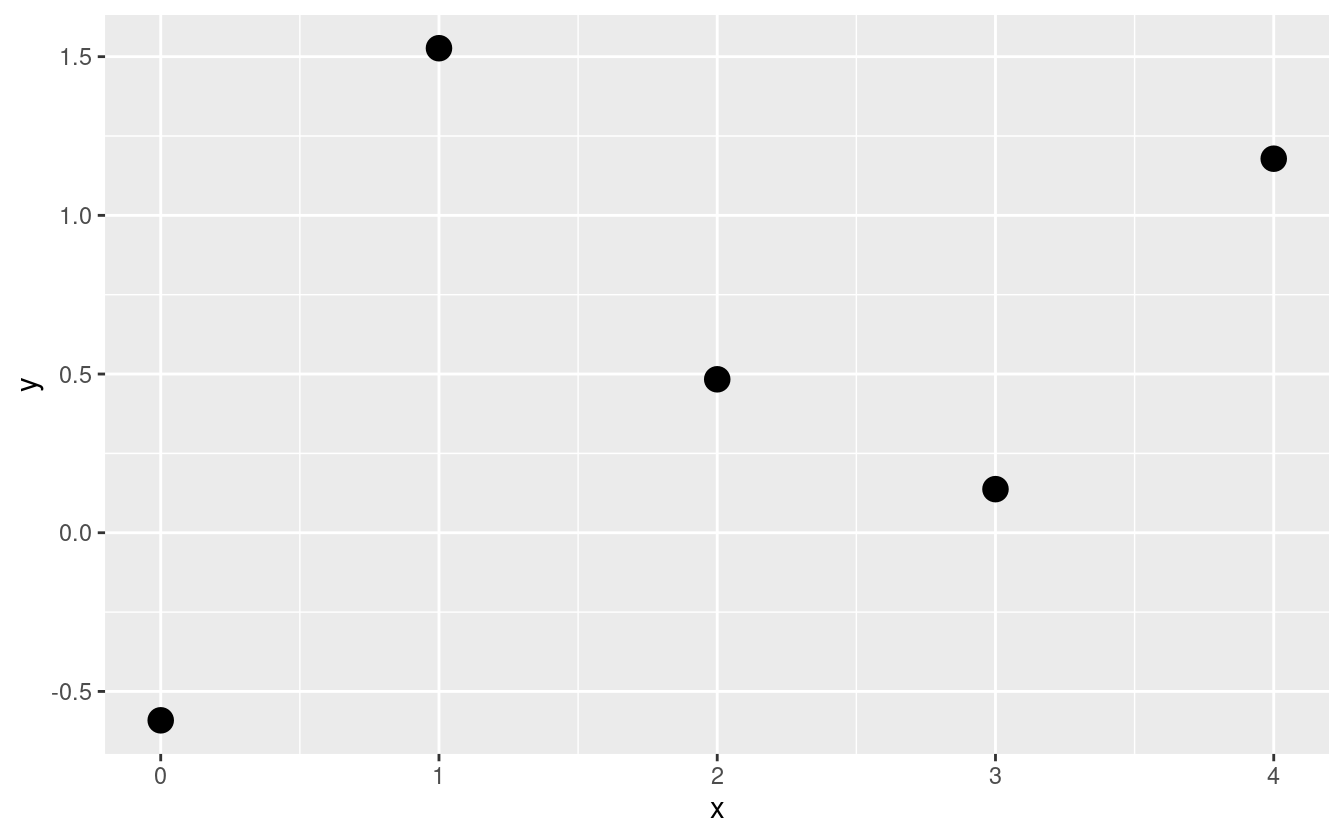
\includegraphics[width=0.85\linewidth]{050-predictive-inference_files/figure-latex/ch050-Moving-Moose-1} 

}

\caption{Five points from a polynomial model.}\label{fig:ch050-Moving-Moose}
\end{figure}

One thing to try is fit a handful of linear models, check the parameter's p-values, the \(R^2\) statistic, and perform other goodness of fit tests, but there is a problem. As you increase the degree of the polynomial fit, the \(R^2\) statistic will always increase. In fact with five data points, a fourth degree polynomial will fit the data perfectly (figure \ref{fig:ch050-Olive-Screwdriver}).

\begin{figure}

{\centering 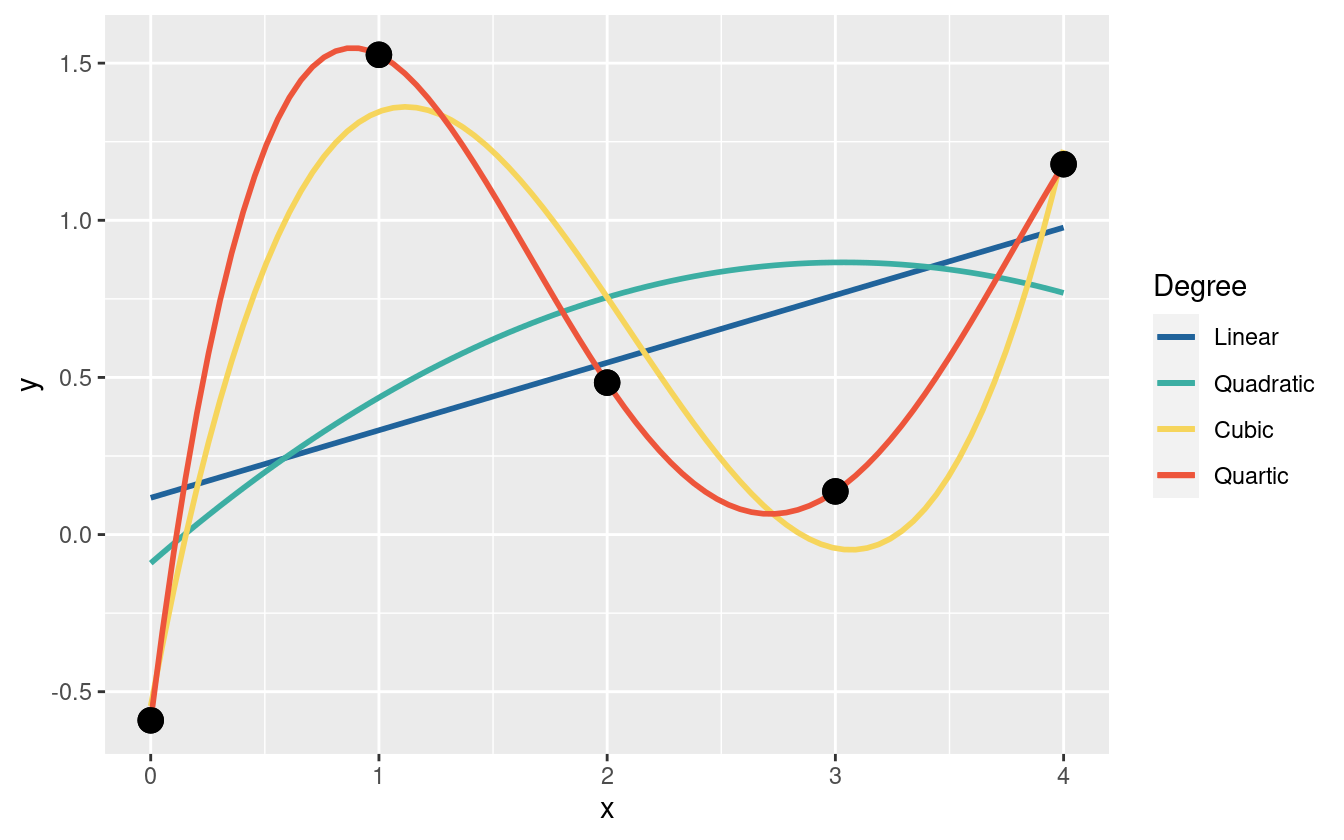
\includegraphics[width=0.85\linewidth]{050-predictive-inference_files/figure-latex/ch050-Olive-Screwdriver-1} 

}

\caption{Data points with various polynomial regression lines.}\label{fig:ch050-Olive-Screwdriver}
\end{figure}

If I were to add a \(6^{th}\) point - a new observation - which of the models would you expect to do best? Can it be estimated which model will predict best before testing with new data? One guess is that the quadratic or cubic model will do well because because the linear model is potentially \emph{underfit} to the data and the quartic is \emph{overfit} to the data. Figure \ref{fig:ch050-Cold-Fish} shows the new data point from the polynomial model. Now the linear and cubic models are trending in the wrong direction. The quadratic and quartic models are both trending down, so may be the correct form for the model.

\begin{figure}

{\centering 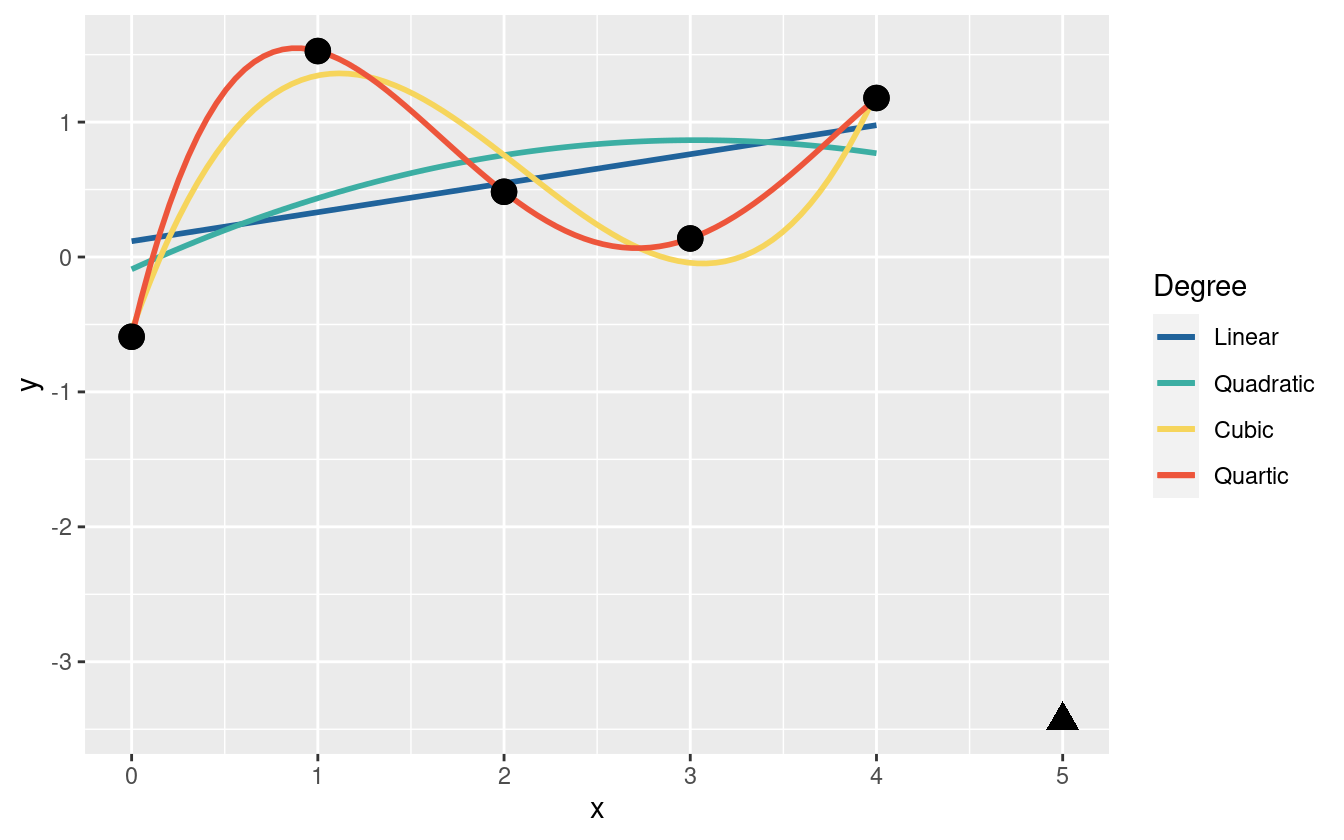
\includegraphics[width=0.85\linewidth]{050-predictive-inference_files/figure-latex/ch050-Cold-Fish-1} 

}

\caption{The fitted polynomial models with a new observation.}\label{fig:ch050-Cold-Fish}
\end{figure}

Figure \ref{fig:ch050-Strawberry-Swallow} shows the 80\% and 95\% prediction intervals for a new observation given \(x = 5\) as well as the true outcome as a dashed line at \(y = -3.434\). The linear model has the smallest prediction interval (PI), but completely misses the target. The remaining three models all include the observed value in their 95\% PIs, but the quadratic has the smallest PI of the three. The actual data generating polynomial is

\begin{align*}
y &\sim \mathcal{N}(\mu, 1^2) \\
\mu &= -0.5(x - 2)^2 + 2
\end{align*}

\textbackslash begin\{figure\}

\{\centering 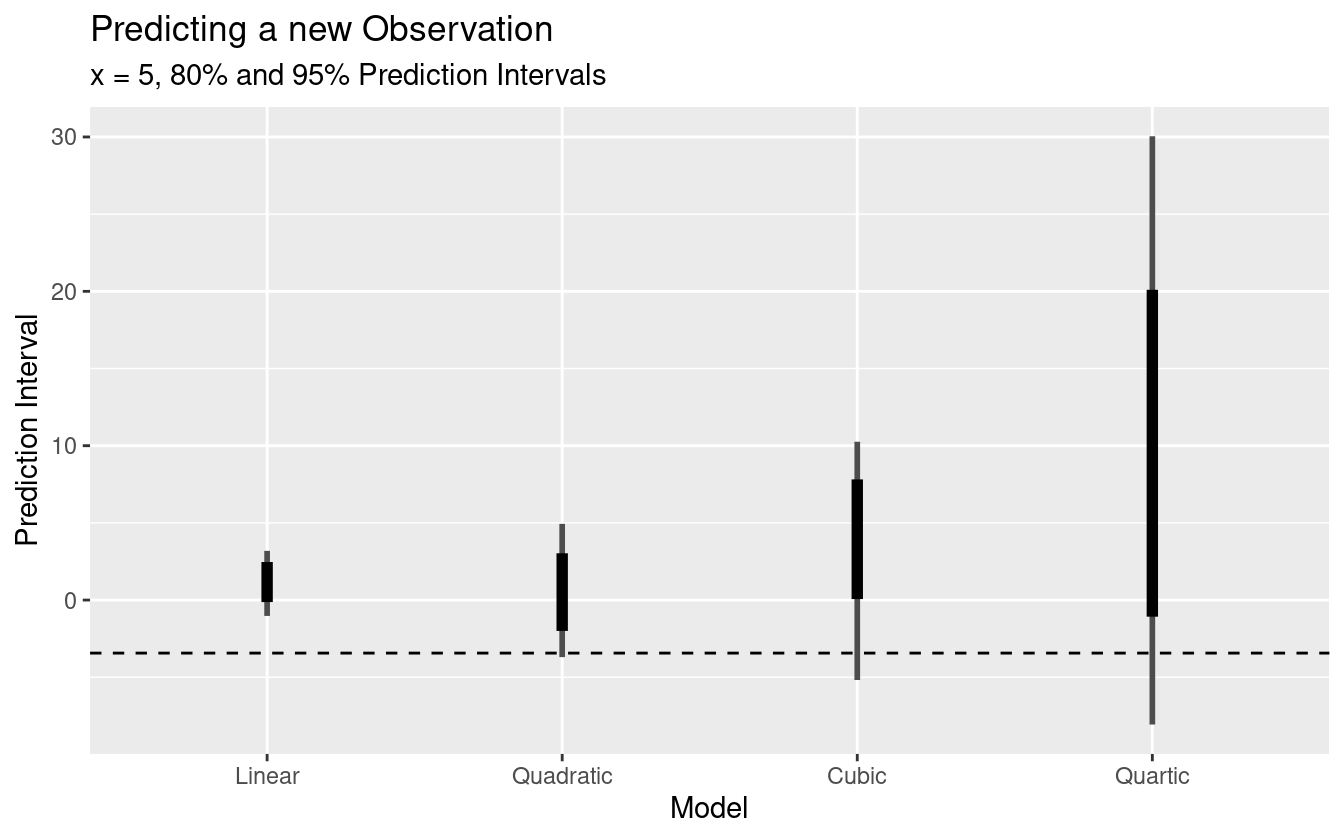
\includegraphics[width=0.85\linewidth]{050-predictive-inference_files/figure-latex/ch050-Strawberry-Swallow-1}

\}

\textbackslash caption\{95\% Prediction intervals for the four polynomial models, as well as the true value (dashed line).\}\label{fig:ch050-Strawberry-Swallow}
\textbackslash end\{figure\}

This is just a toy example, and real-world real-data models are often more complex, but they do present the same headaches when it comes to model/feature selection and goodness of fit checks. Clearly the quartic model has the best fit to the data, but it is too variable and doesn't capture the regular features of the data, so it does poorly for the out-of-sample prediction. The linear model suffers as well by being less biased and too inflexible to capture the structure of the data. The quadratic and cubic are in the middle of the road, but the quadratic does well and makes fewer assumptions about the data. In other words, the quadratic model is just complex enough to predict well while making fewer assumptions. \emph{Information criteria} is a way of weighing the prediction quality of a model against its complexity, and is arguably a better system for model selection/comparison than other goodness of fit statistics such as \(R^2\) or p-values.

\hypertarget{model-comparison-via-predictive-performance}{%
\section{Model Comparison via Predictive Performance}\label{model-comparison-via-predictive-performance}}

We don't always have the observed data to compare predictions against (nor the data generating model). Some techniques to compensate for this limitation include cross validation, where the data is split into \emph{training} data and \emph{testing} data. The model is fit to the training data, and then predictions are made with the testing data and compared to the observed values. This can often give a good estimate for out-of-sample prediction error. Cross validation can be extended into k-fold cross validation. The idea is to \emph{fold} the data into \(k\) disjoint partitions, and predict partition \(i\) using the rest of the data to train on. The prediction error of the \(k\)-folds can then be averaged over to get an estimate for out-of-sample prediction error.

Taking \(k\)-fold CV to the limit by letting \(k = \# observations\) results in something called \emph{leave one out cross validation} (LOOCV), where for each observation in the data, the model is fit to the remaining data and predicted for the left out observation. The downside of \(k\)-fold cross validation is that it requires fitting the model \(k\) times, which can be computationally expensive for complex Bayesian models. Thankfully there is a way to approximate LOOCV without having to refit the model many times.

\hypertarget{loocv-and-importance-sampling}{%
\subsection{LOOCV and Importance Sampling}\label{loocv-and-importance-sampling}}

LOOCV and many other evaluation tools such as WAIC rest on the \emph{log-pointwise-predictive-density} (lppd), which is a loose measure of deviance from some ``true'' probability distribution. Typically we don't have the analytic form of the predictive posterior, so instead we use \(S\) MCMC draws to approximate the lppd \citep{vehtari2017practical}:

\begin{equation}
\mathrm{lppd}(y, \Theta) = \sum_i \log \frac{1}{S} \sum_s p(y_i | \Theta_s)
\label{eq:lppd}
\end{equation}

To estimate LOOCV, the relative ``importance'' of each observation must be computed. Certain observations have more influence on the posterior distribution, and so have more impact on the posterior if they are removed. The intuition behind measuring importance is that more influential observations are relatively less likely than less important observations that are relatively expected. Then by omitting a sample, the relative importance weight can be measured by the lppd. This omitted calculation is known as the out-of-sample lppd. For each omitted \(y_i\),

\[
\mathrm{lppd}_{CV} = \sum_i \frac{1}{S} \sum_s \log p(y_{i} | \Theta_{-i,s})
\]

There is a package called \texttt{loo} that can compute the expected log-pointwise-posterior-density (ELPD) using PSIS-LOO, as well as the estimated number of effective parameters and LOO information criterion \citep{R-loo}. For the part of the researcher, the log-likelihood of the observations must be computed in the model. For my models, I added this in the \emph{generated quantities} block of my Stan program. It is standard practice to name the log-likelihood as \texttt{log\_lik} in the model.

\begin{verbatim}
generated quantities {
  vector[N] log_lik;

  for (i in 1:N) {
    real alpha = b + bGT[G[i], trt[i]];
    real beta = a + aGT[G[i], trt[i]];
    real lambda = lG[G[i]];
    real p = lambda + (1 - 2*lambda) * inv_logit(exp(beta) * (x[i] - alpha));
    log_lik[i] = binomial_lpmf(k[i] | n[i], p);
  }
}
\end{verbatim}

Models can be compared simply using \texttt{loo::loo\_compare}. It estimated the ELPD and its standard error, then calculates the relative differences between all the models. The model with the highest ELPD is predicted to have the best out-of-sample predictions. The comparison of the first three iterations of the model from \protect\hyperlink{workflow}{chapter 3} for the audiovisual data are shown below.

\begin{Shaded}
\begin{Highlighting}[]
\NormalTok{comp_av <-}\StringTok{ }\KeywordTok{loo_compare}\NormalTok{(l031_av, l032_av, l032nc_av, l033_av)}
\KeywordTok{print}\NormalTok{(comp_av, }\DataTypeTok{simplify =} \OtherTok{FALSE}\NormalTok{)}
\CommentTok{#>        elpd_diff se_diff elpd_loo se_elpd_loo p_loo   se_p_loo looic   se_looic}
\CommentTok{#> model4     0.0       0.0 -1615.7     42.8        16.2     0.9   3231.4    85.6 }
\CommentTok{#> model2    -1.0       3.8 -1616.7     42.6        11.3     0.6   3233.3    85.2 }
\CommentTok{#> model3    -1.3       3.8 -1617.0     42.7        11.8     0.6   3234.0    85.3 }
\CommentTok{#> model1   -32.8      10.4 -1648.5     43.0         3.0     0.2   3296.9    86.1}
\end{Highlighting}
\end{Shaded}

The centered and non-centered parameterizations (models 2 and 3 respectively) have essentially the same ELPD. This is expected since they are essentially the same model. The reparameterization only helps with model fitting efficiency, though that can mean more reliable posteriors. The model with age-block interactions (model 4) has the highest ELPD, but is not decisively the best as determined by the standard error of the ELPD. The only thing that can be determined is that including age and block improves performance significantly over the base model (model 1).

But how about for the visual data? The fourth iteration of the model introduced a lapse rate. Did the change significantly improve the ELPD?

\begin{Shaded}
\begin{Highlighting}[]
\NormalTok{comp_vis <-}\StringTok{ }\KeywordTok{loo_compare}\NormalTok{(l033_vis, l034_vis)}
\KeywordTok{print}\NormalTok{(comp_vis, }\DataTypeTok{simplify =} \OtherTok{FALSE}\NormalTok{)}
\CommentTok{#>        elpd_diff se_diff elpd_loo se_elpd_loo p_loo   se_p_loo looic   se_looic}
\CommentTok{#> model2     0.0       0.0 -1001.1     44.0        19.2     1.9   2002.2    88.0 }
\CommentTok{#> model1  -259.4      31.9 -1260.5     56.1        23.1     2.3   2520.9   112.2}
\end{Highlighting}
\end{Shaded}

Absolutely! Something else interesting also happened with the introduction of the lapse rate - the effective number of parameters decreased (\texttt{p\_loo}).

Earlier I argued that model selection is out, model comparison is in. At the end of \protect\hyperlink{workflow}{chapter 3} I finished with a model that has age-block interactions and a lapse rate for each age group. There was one more model that I could have specified - one that estimates at the subject level. There is no domain-specific reason to include the subject level information, especially since the goal is to make inferences at the age group level, but there may still be statistical reason to add in the subjects. For one, adding in the subject as another level in a multilevel model can induce regularization among the subjects, which can overall make for better predictions on new data.

I've gone ahead and fit the model with subject-level information, and the comparison between this new model and the one from iteration 4 is shown below.

\begin{Shaded}
\begin{Highlighting}[]
\NormalTok{comp_vis2 <-}\StringTok{ }\KeywordTok{loo_compare}\NormalTok{(l034_vis, l034s_vis)}
\KeywordTok{print}\NormalTok{(comp_vis2, }\DataTypeTok{simplify =} \OtherTok{FALSE}\NormalTok{)}
\CommentTok{#>        elpd_diff se_diff elpd_loo se_elpd_loo p_loo   se_p_loo looic   se_looic}
\CommentTok{#> model2     0.0       0.0  -925.1     38.1        75.6     5.4   1850.3    76.2 }
\CommentTok{#> model1   -76.0      19.1 -1001.1     44.0        19.2     1.9   2002.2    88.0}
\end{Highlighting}
\end{Shaded}

Including the subject-level information significantly improves the ELPD, and even though there are over 100 parameters in the model (slope and intercept for each of the 45 subjects), the effective number of parameters is much less. Since this new model is capable of making inferences at both the age group level and the subject level, I use it for the result section (\protect\hyperlink{results}{chapter 6}).

One concern comes up when it comes to LOOCV and multilevel models. What does it mean to leave \emph{one} out? Should one subject be left out? One age group? Just one observation? With more levels in a model, more careful considerations must be taken when it comes to estimating prediction performance.

\hypertarget{results}{%
\chapter{Psychometric Results}\label{results}}

What was the point of going through all the work of building a model if not to answer the questions that motivated the model in the first place? To reiterate, the questions pertain to how the brain reconciles stimuli originating from different sources, and if biological (age) and contextual (task, temporal recalibration) factors contribute to global percepts. The way through which these questions are answered is through a psychometric experiment and the resulting psychometric function (\protect\hyperlink{motivating-data}{chapter 2}). I've divided this chapter into two sections - the affects of temporal recalibration and the consideration of a lapse rate. Temporal recalibration is considered in the context of perceptual synchrony and temporal sensitivity, and the results are broken down by age group. Also recall that there are four separate tasks - audiovisual, visual, duration, and sensorimotor.

\hypertarget{affect-of-adaptation-across-age-groups}{%
\section{Affect of Adaptation across Age Groups}\label{affect-of-adaptation-across-age-groups}}

Temporal recalibration consists of presenting a subject with an adapting stimulus throughout a block of a psychometric experiment. Depending on the mechanisms at work, the resulting psychometric function can either be shifted (biased) towards the adapting stimulus (lag adaption) or away (Bayesian adaptation). The theory of integrating sensory signals is beyond my scope, but some papers discussing sensory adaptation in more detail are \citet{miyazaki2006bayesian}, \citet{sato2011bayesian}, and \citet{stocker2005sensory}. I will be discussing the statistical results without considering the deeper psychological theory.

\hypertarget{on-perceptual-synchrony}{%
\subsection{On Perceptual Synchrony}\label{on-perceptual-synchrony}}

Perceptual synchrony is when the temporal delay between two stimuli is small enough so that the brain integrates the two signals into a global percept - perceived as happening simultaneously. Perceptual synchrony is studied through the point of subjective simultaneity (PSS), and in a simple sense represents the bias towards a given stimulus. Ideally the bias would be zero, but human perception is liable to change due to every day experiences. The pre-adaptation block is a proxy for implicit bias, and the post-adaptation indicates whether lag or Bayesian adaptation is taking place. Some researchers believe that both forms of adaptation are taking place at all times and that the mixture rates are determined by biological and contextual factors. I will try to stay away from making any strong determinations and will only present the results conditional on the model and the data.

\textbf{Audiovisual TOJ Task}

There are two ways that we can visually draw inferences across the 6 different age-block combinations. The distributions can either be faceted by age group, or they can be faceted by block. There are actually many ways that the data can be presented, but these two methods of juxtaposition help to answer two questions - how does the effect of adaptation vary by age group, and is there a difference in age groups by block? The left hand plot of figure \ref{fig:ch060-Eastern-Cat} answers the former, and the right hand plot answers the latter.

\begin{figure}

{\centering 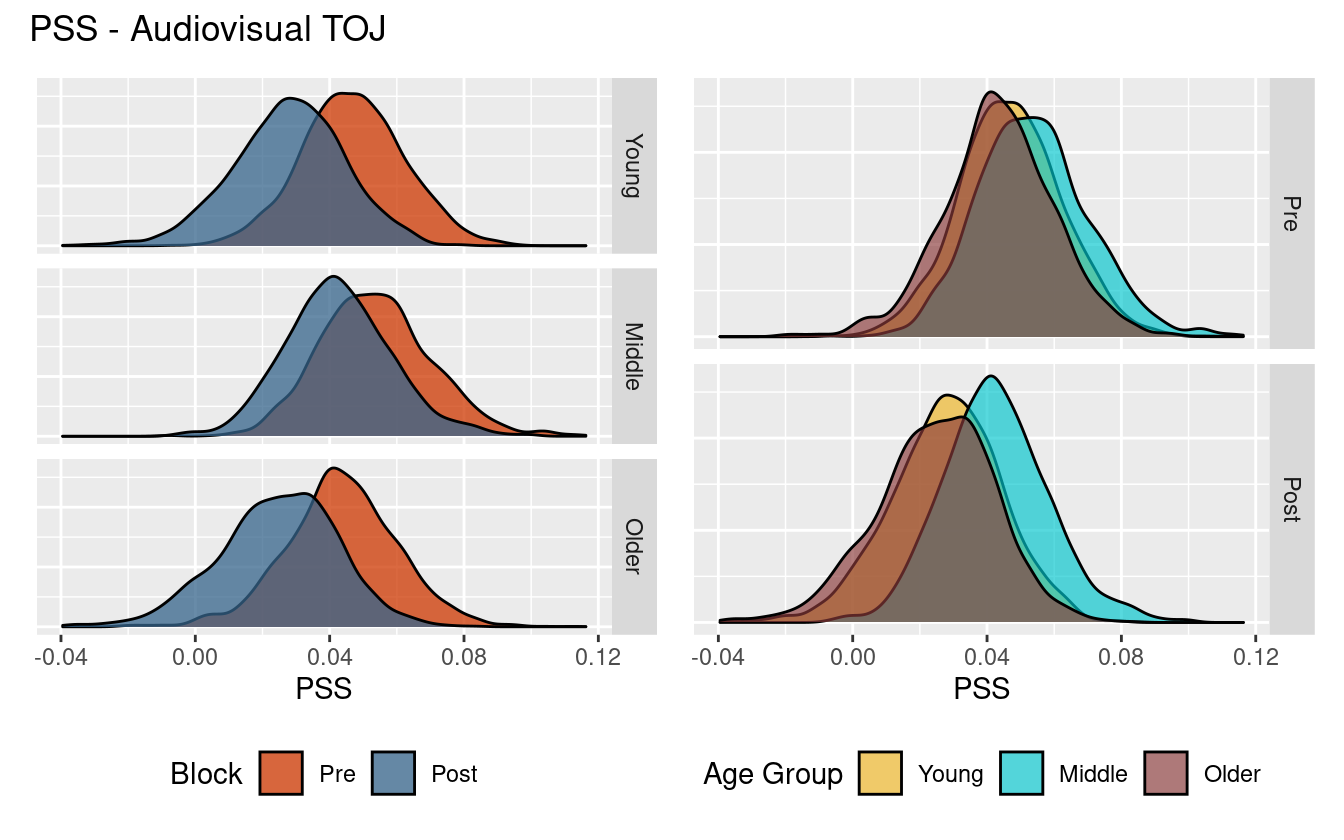
\includegraphics[width=0.85\linewidth]{060-results_files/figure-latex/ch060-Eastern-Cat-1} 

}

\caption{Posterior distribution of PSS values for the audiovisual task.}\label{fig:ch060-Eastern-Cat}
\end{figure}

Across all age groups, temporal recalibration results in a negative shift towards zero in the PSS (as shown by the left hand plot), but there is no significant difference in the PSS between age groups (right hand plot). A very convenient consequence of using MCMC is that the samples from the posterior can be recombined in many ways to describe new phenomena. The PSS values can even be pooled across age groups so that the marginal affect of recalibration may be considered (left hand plot of figure \ref{fig:ch060-Beta-Lonesome}).

\begin{figure}

{\centering 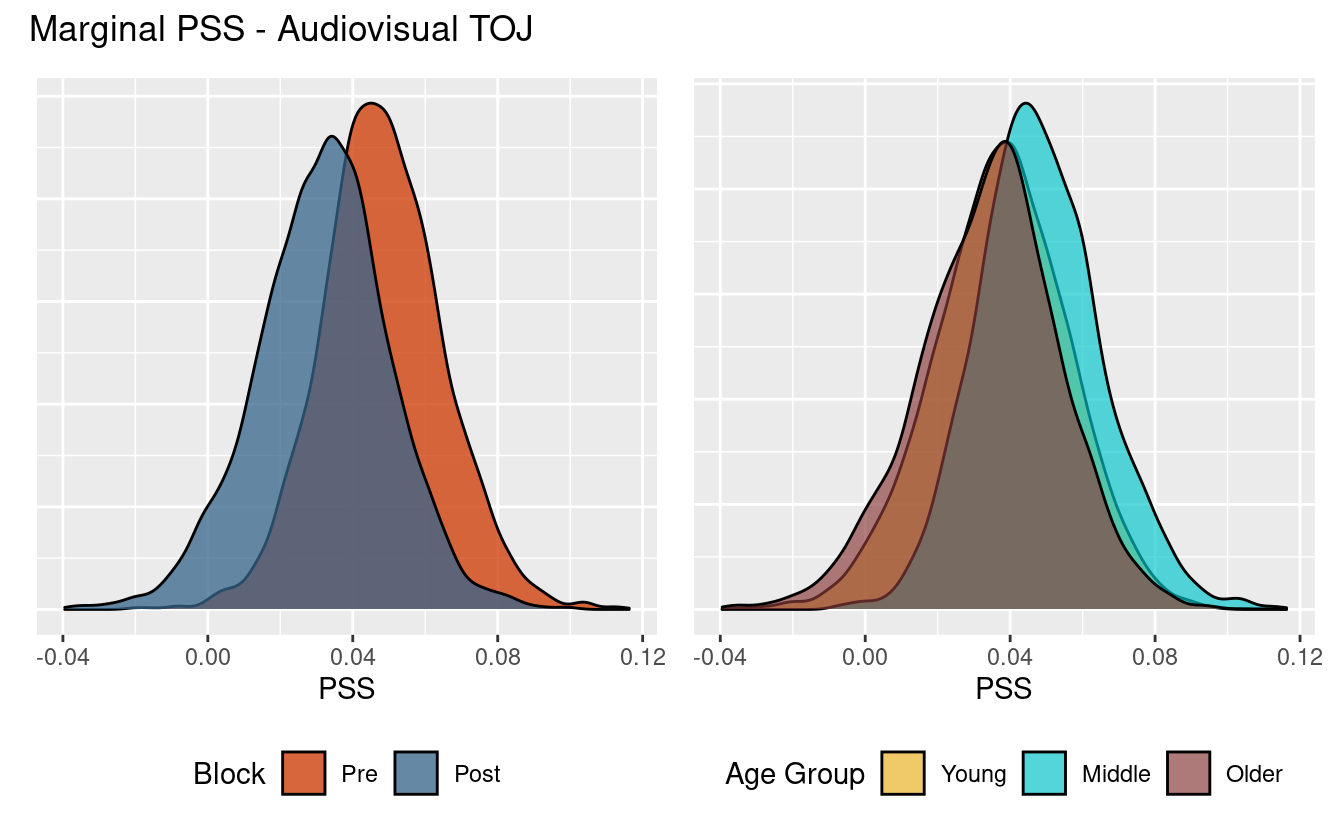
\includegraphics[width=0.85\linewidth]{060-results_files/figure-latex/ch060-Beta-Lonesome-1} 

}

\caption{Posterior distribution of PSS values for the audiovisual task. Left: Marginal over age group. Right: Marginal over block.}\label{fig:ch060-Beta-Lonesome}
\end{figure}

Now with the marginal of age group, the distribution of differences between pre- and post-adaptation blocks can be calculated. I could report a simple credible interval, but it almost seems disingenuous given that the entire distribution is available. I could report that the \(90\%\) highest posterior density interval (HPDI) of the difference is \((-0.036, 0.003)\), but consider the following figure instead.

\textbackslash begin\{figure\}

\{\centering 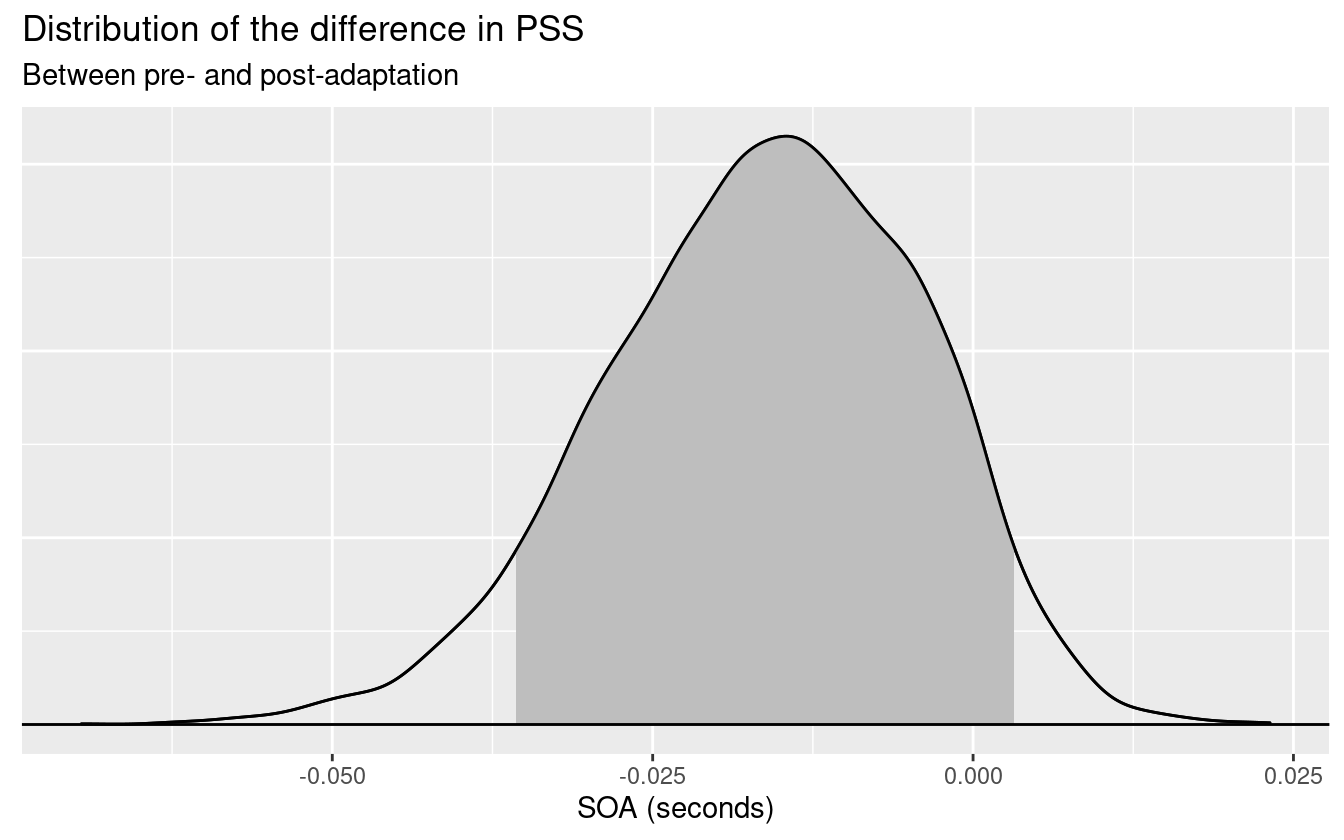
\includegraphics[width=0.85\linewidth]{060-results_files/figure-latex/ch060-Omega-Permanent-1}

\}

\textbackslash caption\{Distribution of differences for pre- and post-adaptation PSS values with 90\% HPDI.\}\label{fig:ch060-Omega-Permanent}
\textbackslash end\{figure\}

Figure \ref{fig:ch060-Omega-Permanent} shows the distribution of differences with the \(90\%\) HPDI region shaded. From this figure, one might conclude that the effect of recalibration, while small, is still noticeable for the audiovisual task. While this could be done for every task in the rest of this chapter, I do not think it is worth repeating as I am not trying to prove anything about the psychometric experiment itself (that is for a later paper). The point of this demonstration is simply that it can be done (and easily), and how to summarize the data both visually and quantitatively.

\textbf{Visual TOJ Task}

\begin{figure}

{\centering 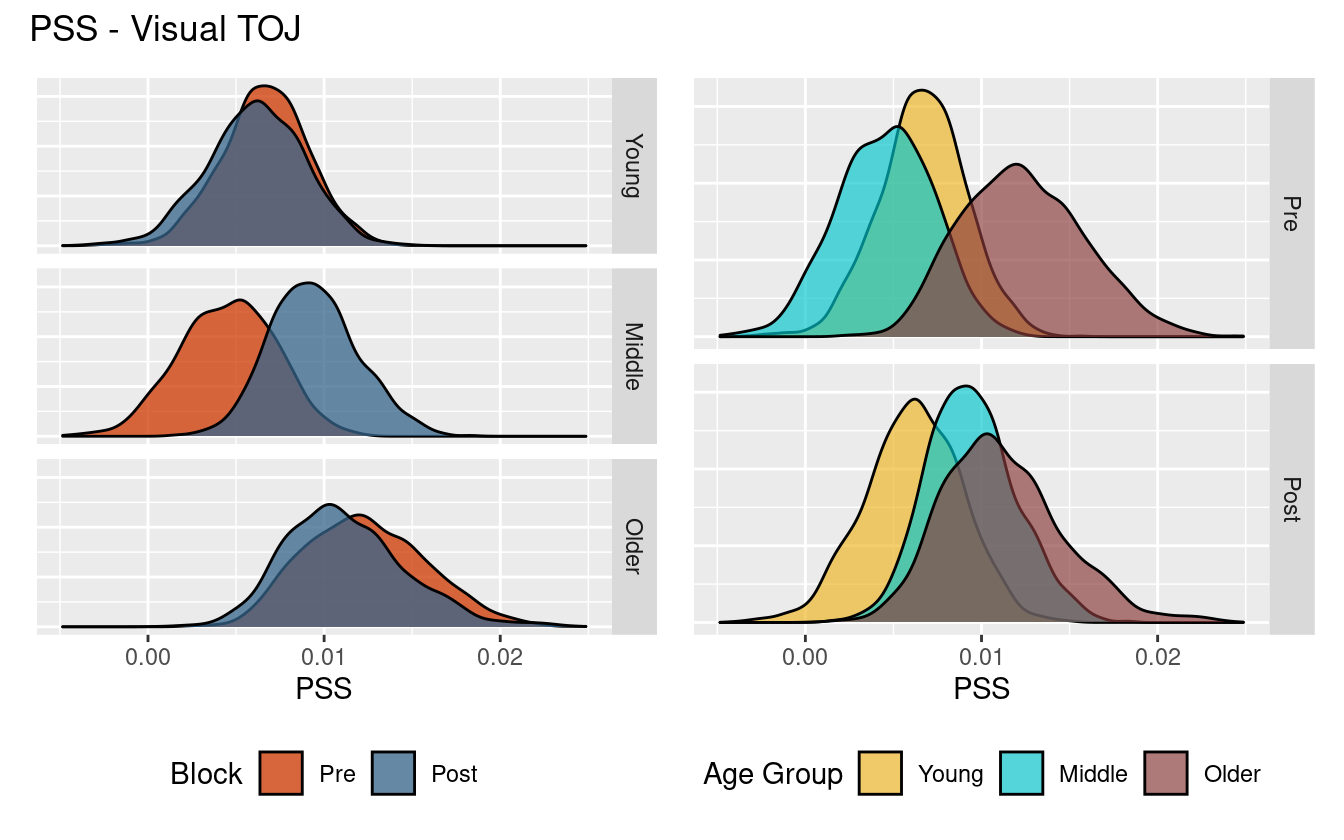
\includegraphics[width=0.85\linewidth]{060-results_files/figure-latex/ch060-Gruesome-Waffle-1} 

}

\caption{Posterior distribution of PSS values for the visual task.}\label{fig:ch060-Gruesome-Waffle}
\end{figure}

Here there is no clear determination if recalibration has an effect on perceptual synchrony, as it is only the middle age group that shows a shift in bias. Even more, there is a lot of overlap between age group. Looking at the marginal distributions (figure \ref{fig:ch060-Cold-Gamma}), there may be a difference between the younger and older age groups, and the middle age and older age groups.

\begin{figure}

{\centering 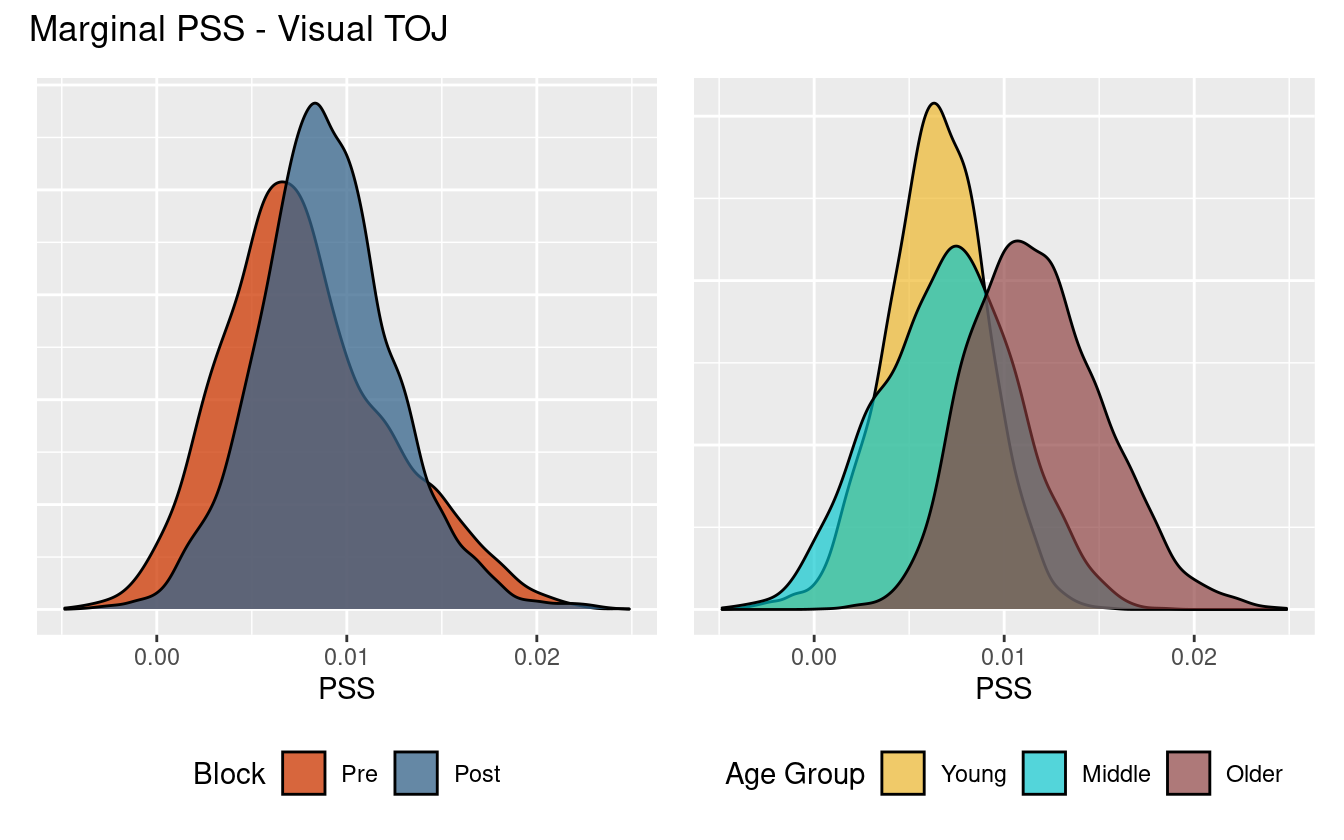
\includegraphics[width=0.85\linewidth]{060-results_files/figure-latex/ch060-Cold-Gamma-1} 

}

\caption{The difference between the older age group and the two others is noticeable, but not likely significant.}\label{fig:ch060-Cold-Gamma}
\end{figure}

These plots are useful for quickly being able to determine if there is a difference in factors. If there is a suspected difference, then the distribution can be calculated from the posterior samples as needed. I suspect that there may be a difference between the older age group and the other two, so I calculated the differences, and summarize them with the histogram in figure \ref{fig:ch060-Rapid-Postal}.

\begin{figure}

{\centering 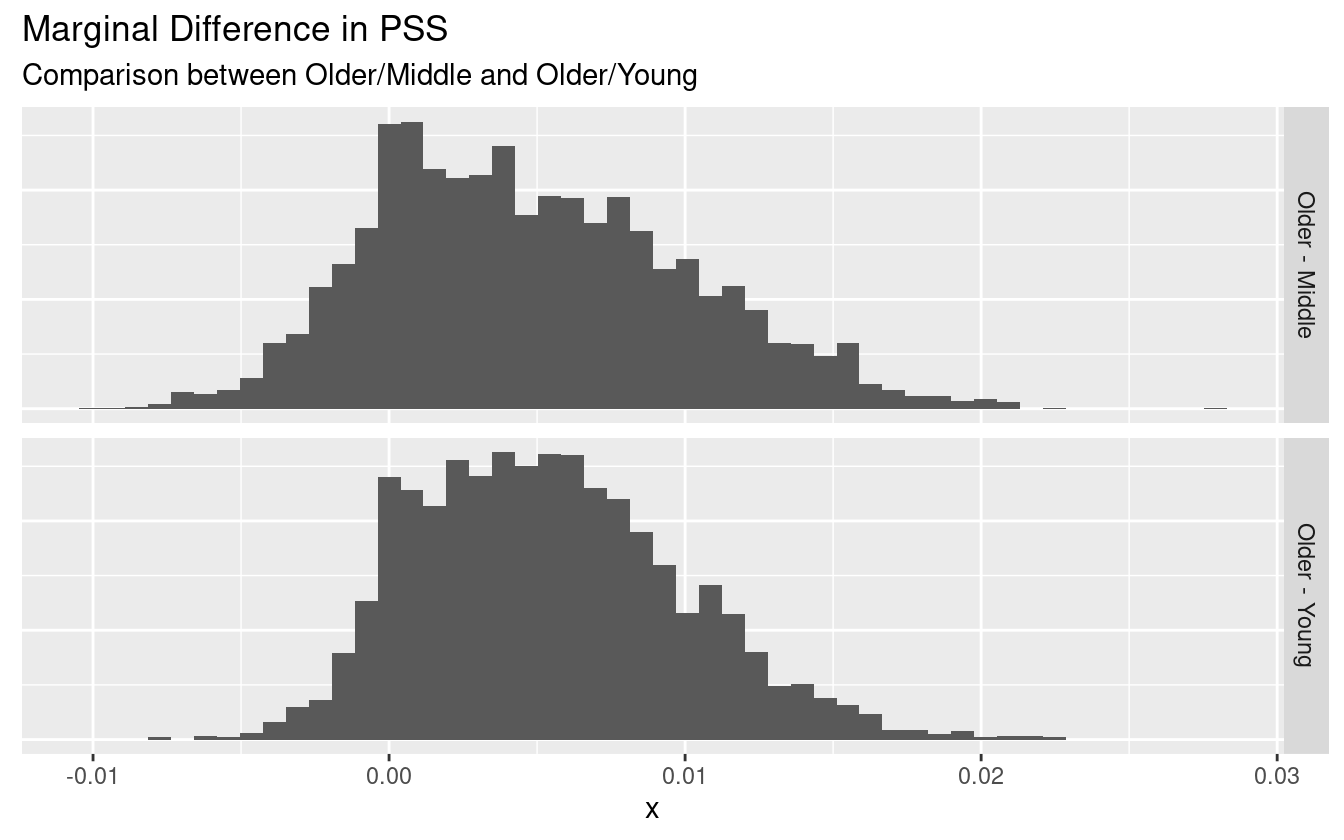
\includegraphics[width=0.85\linewidth]{060-results_files/figure-latex/ch060-Rapid-Postal-1} 

}

\caption{The bulk of the distribution is above zero, but there is still a chance that there is no difference in the distribution of PSS values between the age groups during the visual TOJ experiment.}\label{fig:ch060-Rapid-Postal}
\end{figure}

The bulk of the distribution is above zero, but there is still a chance that there is no difference in the distribution of PSS values between the age groups during the visual TOJ experiment.

\textbf{Duration TOJ Task}

\begin{figure}

{\centering 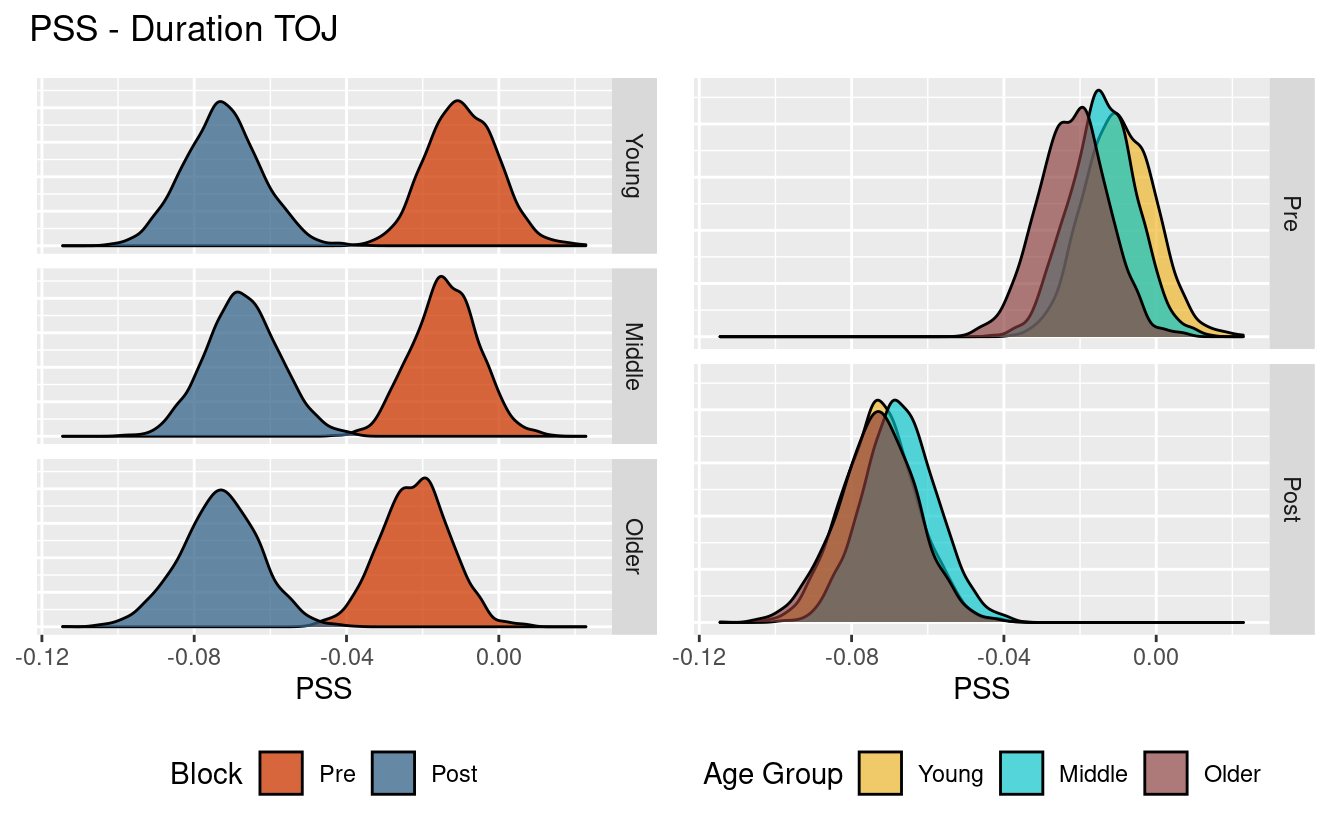
\includegraphics[width=0.85\linewidth]{060-results_files/figure-latex/ch060-Stormy-Frostbite-1} 

}

\caption{Posterior distribution of PSS values for the duration task.}\label{fig:ch060-Stormy-Frostbite}
\end{figure}

The duration TOJ task is very interesting because 1) recalibration had a visually significant effect across all age groups, and 2) there is virtually no difference between the age groups. I could plot the marginal distribution, but it wouldn't likely give any more insight. What I might ask is what is it about the duration task that lets temporal recalibration have such a significant effect? Is human perception of time duration more malleable than our perception to other sensory signals?

\textbf{Sensorimotor TOJ Task}

\begin{figure}

{\centering 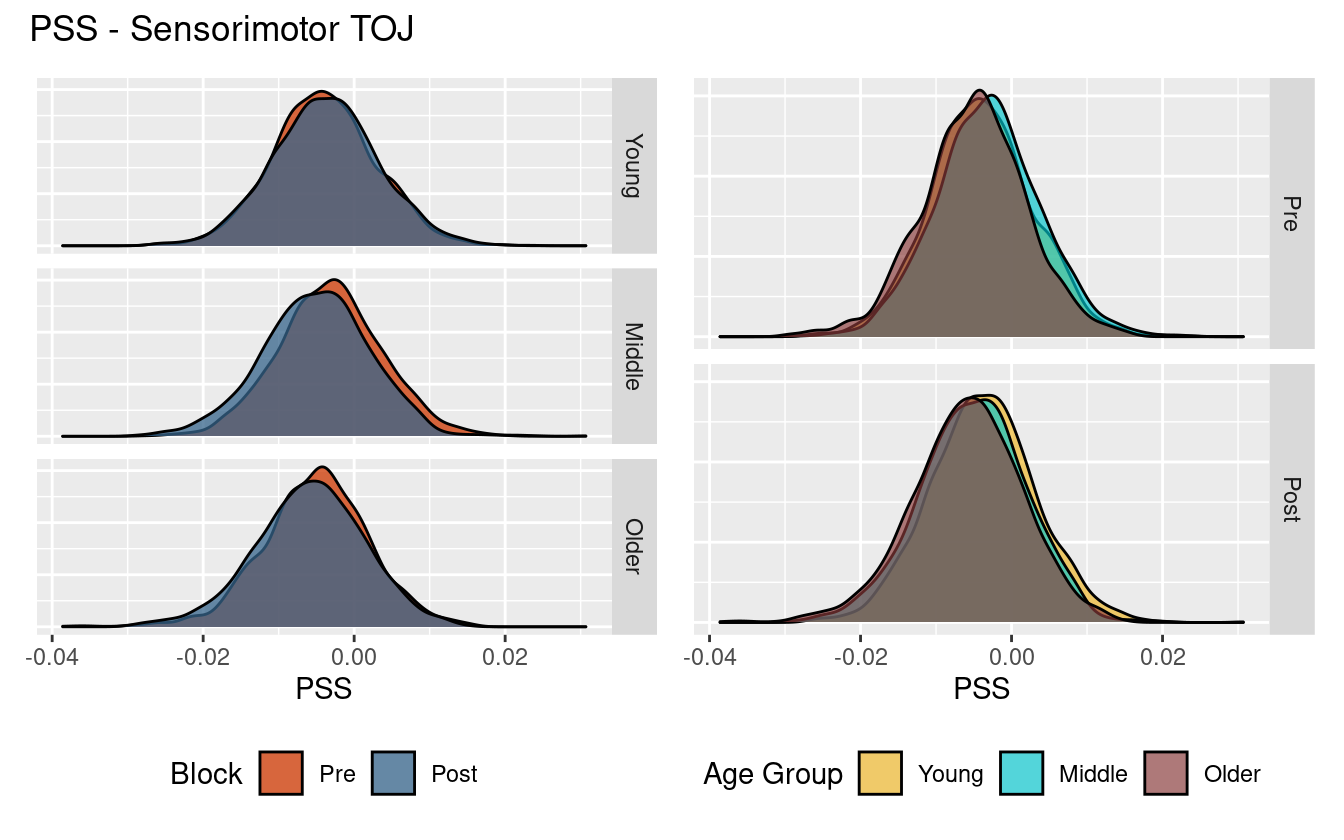
\includegraphics[width=0.85\linewidth]{060-results_files/figure-latex/ch060-Homeless-Anaconda-1} 

}

\caption{Posterior distribution of PSS values for the sensorimotor task.}\label{fig:ch060-Homeless-Anaconda}
\end{figure}

There are no differences between age groups or blocks when it comes to perceptual synchrony in the sensorimotor task.

\hypertarget{on-temporal-sensitivity}{%
\subsection{On Temporal Sensitivity}\label{on-temporal-sensitivity}}

Temporal sensitivity is the ability to successfully integrate signals arising from the same event, or segregate signals from different events. When the stimulus onset asynchrony increases, the ability to bind the signals into a single percept is reduced until they are perceived as distinct events with a temporal order. Those that are more readily able to determine temporal order have a higher temporal sensitivity, and it is measured through the slope of a psychometric function - specifically the quantity known as the just noticeable difference.

\textbf{Audiovisual TOJ Task}

\begin{figure}

{\centering 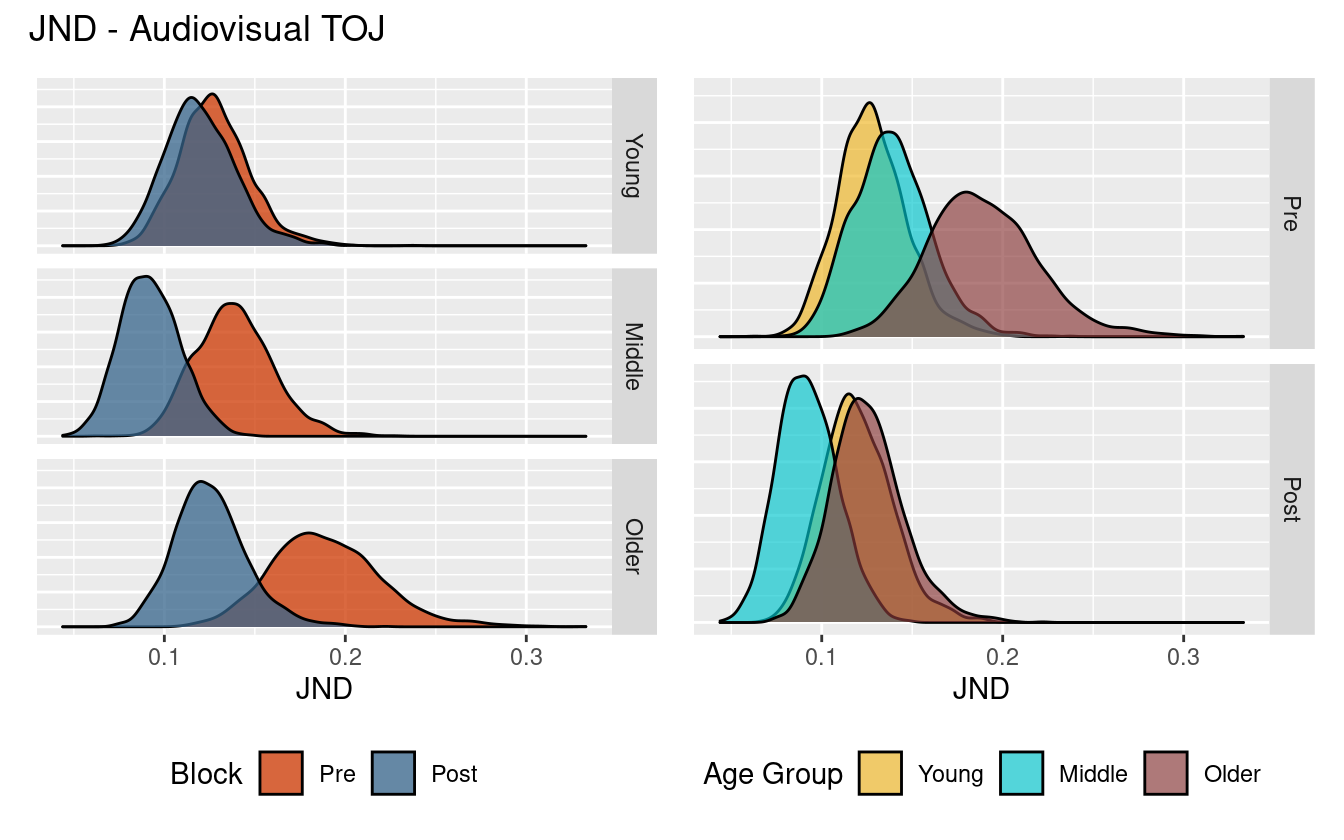
\includegraphics[width=0.85\linewidth]{060-results_files/figure-latex/ch060-Timely-Toupee-1} 

}

\caption{Posterior distribution of JND values for the audiovisual task.}\label{fig:ch060-Timely-Toupee}
\end{figure}

All age groups experienced an increase in temporal sensitivity, but the effect is largest in the older age group which also had the largest pre-adaptation JND estimates. There also appears to be some distinction between the older age group and the younger ones in the pre-adaptation block, but recalibration closes the gap.

\textbf{Visual TOJ Task}

\begin{figure}

{\centering 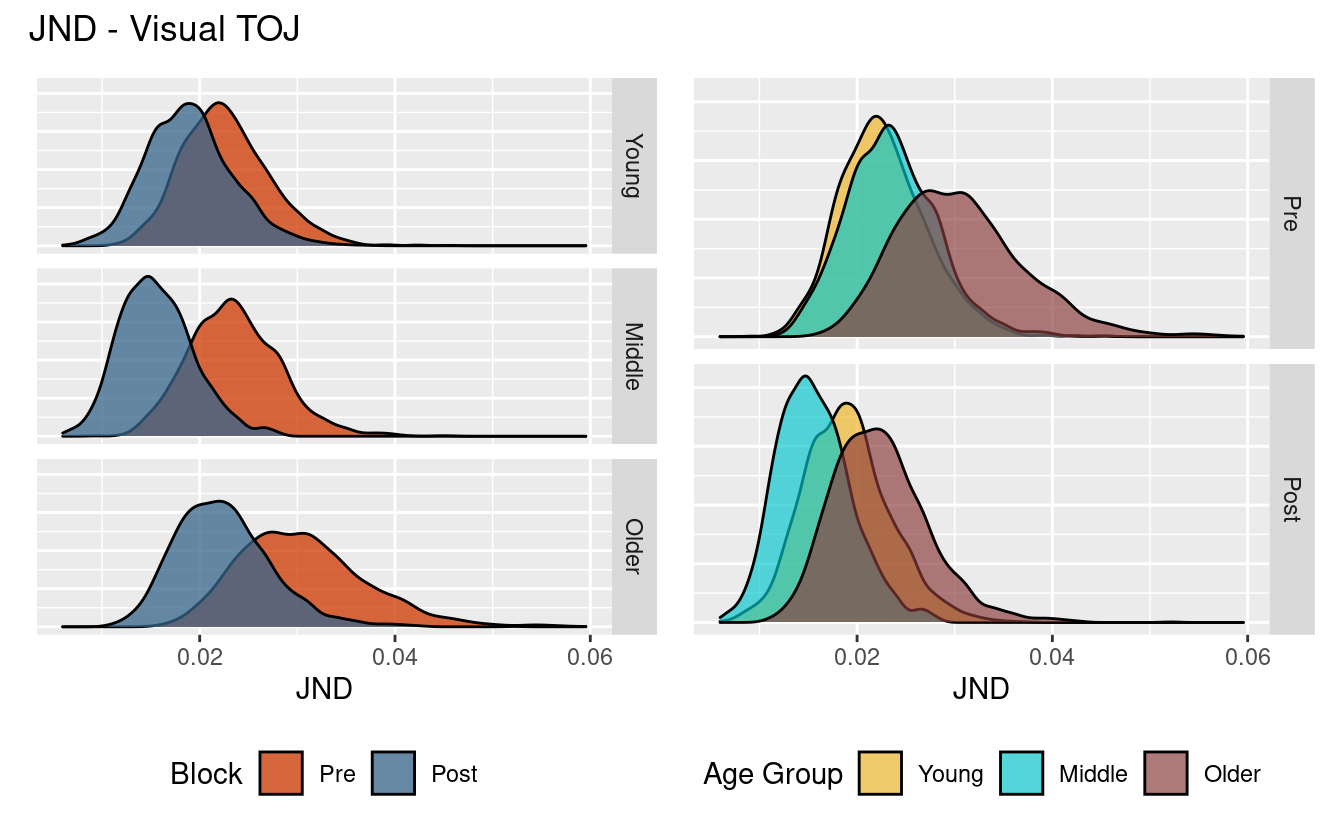
\includegraphics[width=0.85\linewidth]{060-results_files/figure-latex/ch060-Mercury-Rainbow-1} 

}

\caption{Posterior distribution of JND values for the visual task.}\label{fig:ch060-Mercury-Rainbow}
\end{figure}

The story for the visual TOJ task is similar to the audiovisual one - each age group experience heightened temporal sensitivity after recalibration, with the two older age groups receiving more benefit than the younger age group. It's also worth noting that the younger age groups have higher baseline temporal sensitivity, so there may not be as much room for improvement.

\textbf{Duration TOJ Task}

\begin{figure}

{\centering 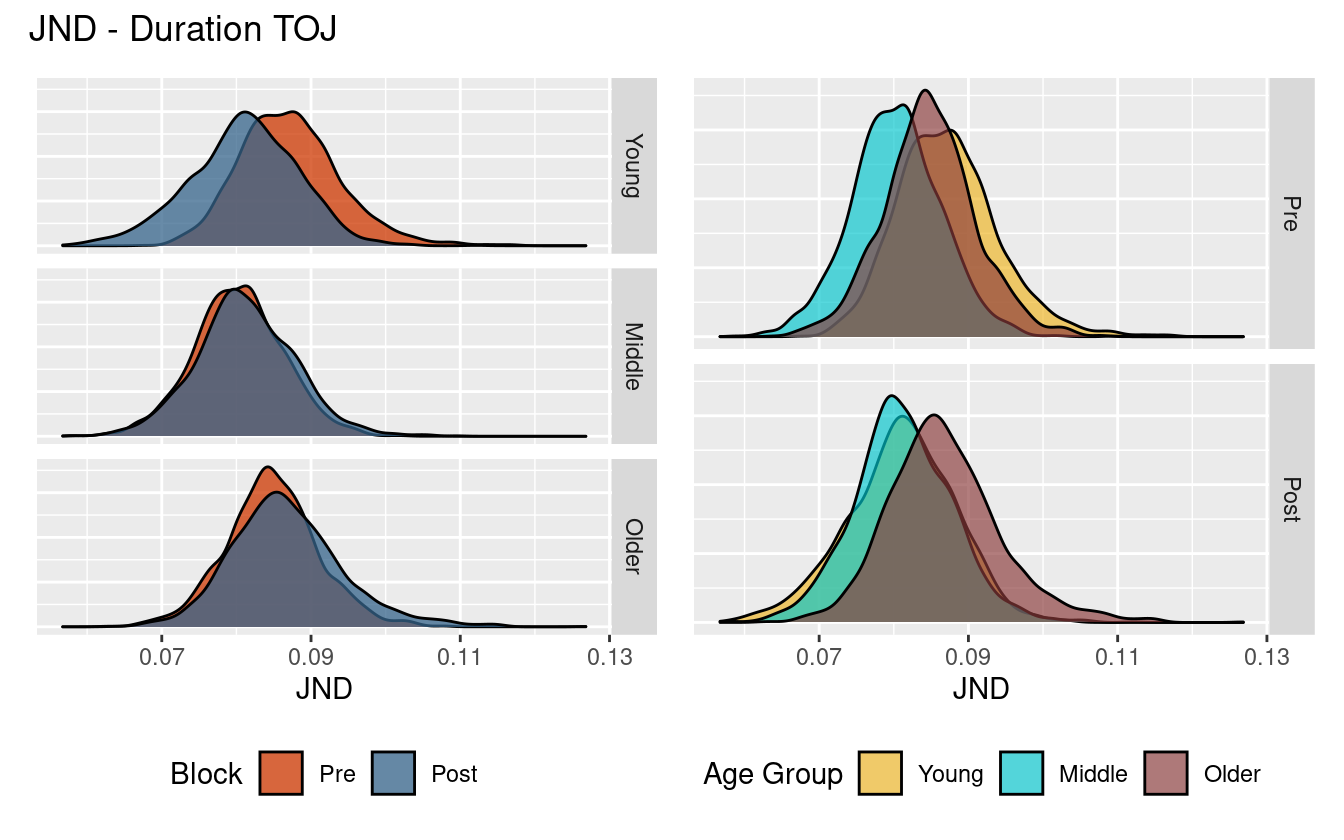
\includegraphics[width=0.85\linewidth]{060-results_files/figure-latex/ch060-Aimless-Planet-1} 

}

\caption{Posterior distribution of JND values for the duration task.}\label{fig:ch060-Aimless-Planet}
\end{figure}

This time the effects of recalibration are not so strong, and just like for the PSS, there is no significant difference between age groups in the duration task.

\textbf{Sensorimotor TOJ Task}

\begin{figure}

{\centering 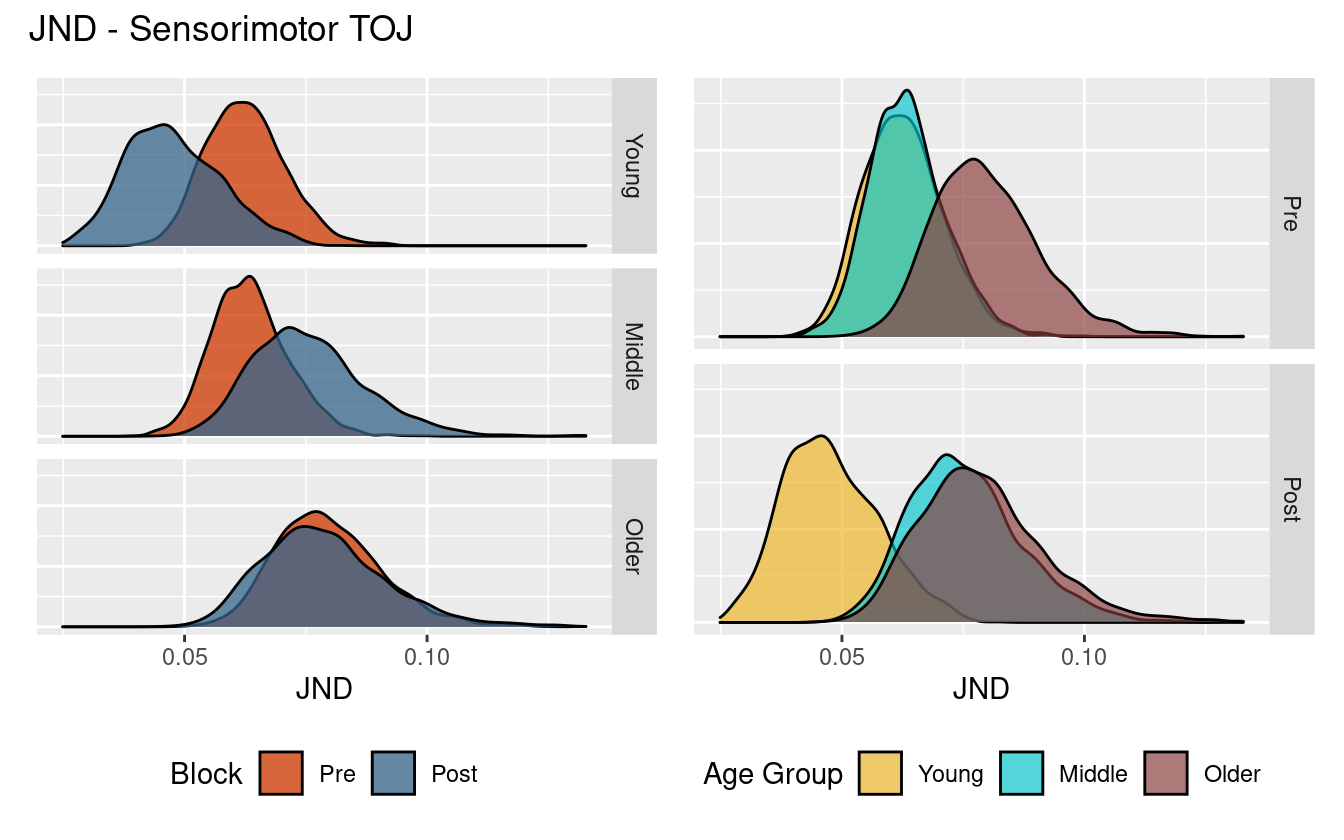
\includegraphics[width=0.85\linewidth]{060-results_files/figure-latex/ch060-Tombstone-Cold-1} 

}

\caption{Posterior distribution of JND values for the sensorimotor task.}\label{fig:ch060-Tombstone-Cold}
\end{figure}

Finally in the sensorimotor task there are mixed results. Temporal recalibration increased the temporal sensitivity in the younger age group, reduced it in the middle age group, and had no effect on the older age group. Clearly the biological factors at play are complex, and the data here is a relatively thin slice of the population. More data and a better calibrated experiment may give better insights into the effects of temporal recalibration.

\hypertarget{lapse-rate-across-age-groups}{%
\section{Lapse Rate across Age Groups}\label{lapse-rate-across-age-groups}}

\begin{figure}

{\centering \includegraphics[width=0.85\linewidth]{060-results_files/figure-latex/ch060-Waffle-Hollow-1} 

}

\caption{Process model of the result of a psychometric experiment with the assumption that lapses occur at random and at a fixed rate, and that the subject guesses randomly in the event of a lapse.}\label{fig:ch060-Waffle-Hollow}
\end{figure}

In the above figure, the outcome of one experiment can be represented as a directed acyclic graph (DAG) where at the start of the experiment, the subject either experiences a lapse in judgment with probability \(\gamma\) or they do not experience a lapse in judgment. If there is no lapse, then they will give a positive response with probability \(F(x)\). If there is a lapse in judgment, then it is assumed that they will respond randomly - e.g.~a fifty-fifty chance of a positive response. In this model of an experiment, the probability of a positive response is the sum of the two paths.

\begin{align}
\mathrm{P}(\textrm{positive}) &= 
  \mathrm{P}(\textrm{lapse}) \cdot \mathrm{P}(\textrm{positive} | \textrm{lapse}) \\
  &\quad + \mathrm{P}(\textrm{no lapse}) \cdot \mathrm{P}(\textrm{positive} | \textrm{no lapse}) \\
  &= \frac{1}{2} \gamma + (1 - \gamma) \cdot F(x)
\end{align}

If we then let \(\gamma = 2\lambda\) then the probability of a positive response becomes

\[
\mathrm{P}(\textrm{positive}) = \lambda + (1 - 2\lambda) \cdot F(x)
\]

This is the lapse model described in \eqref{eq:Psi}! But now there is a little bit more insight into what the parameter \(\lambda\) is. If \(\gamma\) is the true lapse rate, then \(\lambda\) is half the lapse rate. This may sound strange at first, but remember that equation \eqref{eq:Psi} was motivated as a lower and upper bound to the psychometric function, and where the bounds are constrained by the same amount. Here the motivation is from a process model, yet the two lines of reasoning arrive at the same model.

Figure \ref{fig:ch060-Magenta-Finger} shows the distribution of lapse rates for each age group across the four separate tasks. There is no visual trend in the ranks of lapse rates, meaning that no single age group definitively experiences a lower lapse rate than the others, though the middle age group comes close to being the winner and the older age group is more likely to be trailing behind. The distribution of lapse rates does reveal something about the tasks themselves.

\begin{figure}

{\centering 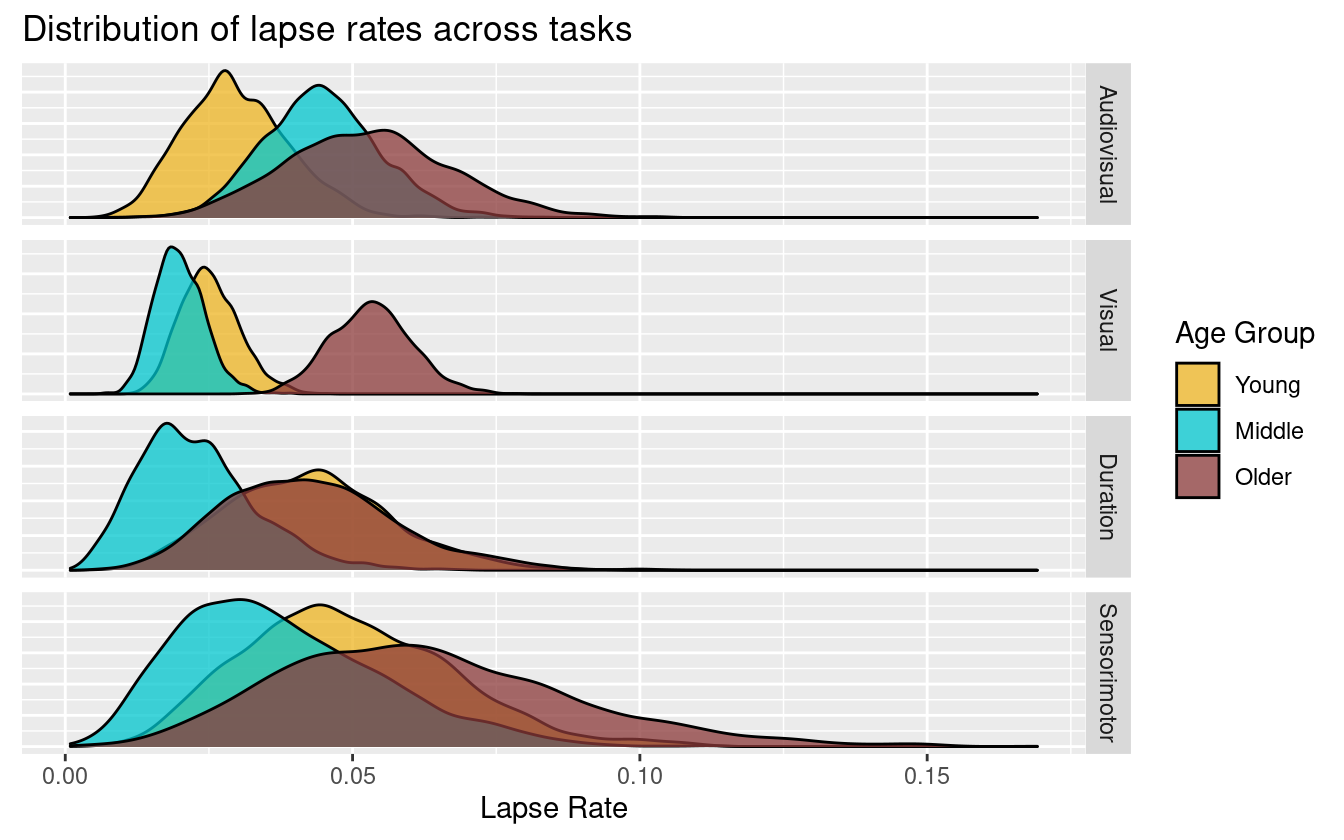
\includegraphics[width=0.85\linewidth]{060-results_files/figure-latex/ch060-Magenta-Finger-1} 

}

\caption{Lapse rates for the different age groups across the four separate tasks. Visually there is no clear trend in lapses by age group, but the concentration of the distributions give insight into the perceived difficulty of a task where more diffuse distributions may indiciate more difficult tasks.}\label{fig:ch060-Magenta-Finger}
\end{figure}

I used the audiovisual data in the first few iterations of building a model and there were no immediate issues, but when I tested the model on the visual data it had trouble expressing the variability at outer SOA values. I noted that one subject had a near perfect response set, and many others had equally impressive performance. The model without a lapse rate was being torn between a very steep slope near the PSS and random variability near the outer SOAs. The remedy was to include a lapse rate (motivated by domain expertise) which allowed for that one extra degree of freedom necessary to reconcile the opposing forces.

Why did the visual data behave this way when the audiovisual data had no issue? That gets deep into the theory of how our brains integrate signals arising from different modalities. Detecting the temporal order of two visual stimuli may be an easier mental task than that of heterogeneous signals. Then consider audiovisual versus duration or sensorimotor. Visual-speech synthesis is a much more common task throughout the day than visual-tactile (sensorimotor), and so perhaps we are better adjusted to such a task as audiovisual. The latent measure of relative performance or task difficulty might be picked up through the lapse rate.

To test this idea, the TOJ experiment could be repeated, and then ask the subject afterwards how they would rate the difficulty of each task. For now, a post-hoc test can be done by comparing the mean and spread of the lapse rates to a \emph{pseuedo difficulty} measure as defined by the mean of the incorrect responses. A response is correct when the sign of the SOA value is concordant with the response, e.g.~a positive SOA and the subject gives the ``positive'' response or a negative SOA and the subject gives the ``negative'' response. Looking at figure \ref{fig:ch060-Magenta-Finger}, I would subjectively rate the tasks from easiest to hardest based on ocular analysis as

\begin{enumerate}
\def\labelenumi{\arabic{enumi}.}
\tightlist
\item
  Visual
\item
  Audiovisual
\item
  Duration
\item
  Sensorimotor
\end{enumerate}

Again, this ranking is based on the mean (lower intrinsically meaning easier) and the spread (less diffuse implying more agreement of difficulty between age groups). The visual task has the tightest distribution of lapse rates, and the sensorimotor has the widest spread, so I can rank those first and last respectively. Audiovisual and duration are very similar in mean and spread, but the audiovisual has a bit more agreement between the young and middle age groups, so second and third go to audiovisual and duration. Table \ref{tab:ch060-Orange-Tigerfish} shows the results arranged by increasing pseudo difficulty. As predicted, the visual task is squarely at the top and the sensorimotor is fully at the bottom. The only out of place group is the audiovisual task for the older age group, which is about equal to the older age group during the duration task. In fact, within tasks, the older age group always comes in last in terms of proportion of correct responses, while the young and middle age groups trade back and forth.

\begin{table}[!h]

\caption{\label{tab:ch060-Orange-Tigerfish}Relative difficulty of the different tasks by age group. The difficulty is measured by the proportion of incorrect responses.}
\centering
\begin{tabular}[t]{l|l|r}
\hline
Task & Age Group & Pseudo Difficulty\\
\hline
visual & Middle Age & 0.03\\
\hline
visual & Young Adult & 0.03\\
\hline
visual & Older Adult & 0.06\\
\hline
audiovisual & Young Adult & 0.12\\
\hline
audiovisual & Middle Age & 0.12\\
\hline
duration & Middle Age & 0.14\\
\hline
duration & Young Adult & 0.16\\
\hline
duration & Older Adult & 0.17\\
\hline
audiovisual & Older Adult & 0.17\\
\hline
sensorimotor & Young Adult & 0.22\\
\hline
sensorimotor & Middle Age & 0.24\\
\hline
sensorimotor & Older Adult & 0.29\\
\hline
\end{tabular}
\end{table}

One way to remove the uncertainty of the lapse rate could be to have some trials with very large SOA values. The reasoning is that if the difficulty of a task (given an SOA value) is lowered, than an incorrect response is more likely to be due to a true lapse in judgment as opposed to a genuinely incorrect response. \citet{wichmann2001b} recommends at least one sample at \(\pi \ge 0.95\) is necessary for reliable bootstrap confidence intervals, so the same reasoning can be applied when using Bayesian credible intervals. For a task such as visual TOJ, the \(90\%\) level may occur at an SOA of \(\approx 40\)ms while for the audiovisual TOJ it may be \(\approx 220\)ms, so the sampling scheme for psychometric experiments must be tuned to the task.

\citet{wichmann2001a} experimentally determined that the lapse rate for trained observers is between \(0\%\) and \(5\%\), and the data in this paper loosely agree with that conclusion. Any excess in lapse rate may be attributed to the perceived task difficulty and a sub-optimal sampling scheme. Since the visual TOJ task is relatively the easiest, the estimated lapse rates are more believable as true lapse rates, and fall closely within the \((0, 0.05)\) range.

\hypertarget{discussion}{%
\chapter{Discussion}\label{discussion}}

\hypertarget{model-selection-is-not-always-the-goal}{%
\section{Model selection is not always the goal}\label{model-selection-is-not-always-the-goal}}

Building a model motivated by a set of principles and domain expertise should be the preferred way of performing an analysis. The next important principle is model comparison, especially in terms of predictive inference. One model also doesn't always work for everything. In the course of building a model that is just complex enough to answer questions about age and temporal recalibration, I mentioned that intermediate models could be used to answer questions about average effects at different levels. For purely predictive inference, there is also the possibility of Bayesian model averaging (BMA) and other ensemble methods.

\hypertarget{data-cleaning-and-reproducibility}{%
\section{Data Cleaning and Reproducibility}\label{data-cleaning-and-reproducibility}}

Data doesn't always come in a nice tidy\footnote{Tidy data is described by Hadley Wickham} format, and I had the pleasure of turning the raw experimental data into a clean data set that is ready for modeling. Sometimes the process is quick and straight forward, but other times, like with this psychometric data, it takes more effort and clever techniques. There is academic value in describing the steps I took up front to reduce the headache later.

To begin, there is a strong push in recent years for reproducible data science. Scientific methods and results should be able to be replicated by other researchers, and part of that includes being able to replicate the process that takes the raw data and produces the tidy data that is ready for analysis. Tidy data is described by \citet{wickham2014tidy} and can be summed up by three principles

\begin{enumerate}
\def\labelenumi{\arabic{enumi}.}
\tightlist
\item
  Each variable forms a column
\item
  Each observation forms a row
\item
  Each type of observational unit forms a table
\end{enumerate}

One problem I have come across and have been guilty of in the past is having data in a spread sheet, modifying it, and then having no way of recovering the original data. Spread sheets are a convenient way to organize, transform, and lightly analyze date, but problems can quickly arise unless there is a good backup/snapshot system in place. Data is immutable\footnote{Mutability in computer science is the property of a data structure where its contents can be modified in place. Immutability means that the object cannot be modified without first making a copy.}, or at least that is the mindset that researchers must adopt in order to have truly reproducible workflows. The raw data that is collected or produced by a measurement device should never be modified without first being copied, even if for trivial reasons such as correcting a spelling mistake\footnote{If a change is made to the raw data, it should be carefully documented and reversible}.

To begin the data cleaning journey, I'll introduce the directory system that I had been given to work with. Each task is separated into its own folder, and within each folder is a subdirectory of age groups.

\begin{center}\includegraphics[width=0.3\linewidth]{figures/data_dir} \end{center}

Within each age group subdirectory are the subdirectories for each subject named by their initials which then contain the experimental data in Matlab files.

\begin{center}\includegraphics[width=0.35\linewidth]{figures/data_subdir} \end{center}

At this point, the data appears manageable, there is information contained in the directory structure such as task, age group, and initials, and file name contains information about the experimental block. There is also an excel file that I was later given that contains more subject information like age and sex, though that information is not used in the model. The columns of the Matlab file depends on the task, but generally contains an SOA value and a response, but no column or row name information - that was provided by the researcher who collected the data.

The next thing I did was to create a table of metadata - information extracted from the directory structure and file names combined with the the subject data and the file path. Regular expressions can be used to extract patterns from a string. With a list of all Matlab files within the \texttt{RecalibrationData} folder, I tried to extract the task, age group, initials, and block using the expression

\begin{verbatim}
"^(\\w+)/(\\w+)/(\\w+)/[A-Z]{2,3}_*[A-Z]*(adapt[0-9]|baseline[0-9]*).*"
\end{verbatim}

Breaking it apart, the \texttt{\^{}(\textbackslash{}\textbackslash{}w+)/} matches any word characters at the start and before the next slash. Since the directory structure is \texttt{Task/AgeGroup/Subject/file.mat}, the regular expression should match three words between slashes. The file name generally follows the pattern of \texttt{Initials\_\_block\#\_\_MAT.mat}, so \texttt{{[}A-Z{]}\{2,3\}\_*{[}A-Z{]}*} should match the initials, and \texttt{(adapt{[}0-9{]}\textbar{}baseline{[}0-9{]}*)} should match the block (baseline or adapt). This method works for \(536\) of the \(580\) individual records. For the ones it failed, it was generally do to misspellings or irregular capitalizing of ``baseline'' and ``adapt''.

\begin{Shaded}
\begin{Highlighting}[]
\KeywordTok{table}\NormalTok{(feat_typ[,}\DecValTok{4}\NormalTok{])}
\CommentTok{#> }
\CommentTok{#>   AC   AG   BB   BC   BT   CB   CC   CE   CJ   CM   DB   DC   DD   DE  DTF   DW }
\CommentTok{#>   13   12   13   13   13   13   10   12   13    4   13   13    7   12   12   13 }
\CommentTok{#>   EM   ET   GB   GT   HG   IV   JM JM_F   JS   JW   KC   KK   LP   MC   MS   MW }
\CommentTok{#>   13   13   13   13   13    4   12   13   13   13   13   11    7   13   13   26 }
\CommentTok{#>   NP   PB   SB   SJ  SJF   TS   TW   VM   WL   WW   YG }
\CommentTok{#>   12   13   12   26   13   13   13   13   13   12    7}
\end{Highlighting}
\end{Shaded}

\begin{Shaded}
\begin{Highlighting}[]
\KeywordTok{table}\NormalTok{(feat_atyp[,}\DecValTok{4}\NormalTok{])}
\CommentTok{#> }
\CommentTok{#>  AG  CC  CE  CM  DD DTF  IV  JM  JS  KK  NP  SB  WW  YG }
\CommentTok{#>   1   3   1   9   6   1   9   1   2   2   1   1   1   6}
\end{Highlighting}
\end{Shaded}

Since there is only a handful of irregular block names, they can be dealt with a separate regular expression that properly extracts the block information. Other challenges in cleaning the data include the handling of subjects with the same initials. This becomes a problem because filtering by a subject's initials is not guaranteed to return a unique subject. Furthermore there are two middle age subjects with the same initials of ``JM'', so one was also identified with their sex ``JM\_F''. The solution is to create a unique identifier (labeled as SID) that is a combination of age group, sex, and initials. For an experiment identifier (labeled as RID), the task and block were prepended to the SID. Each of these IDs uniquely identify the subjects and their experimental records making it easier to filter and search.

\begin{Shaded}
\begin{Highlighting}[]
\KeywordTok{glimpse}\NormalTok{(features)}
\CommentTok{#> Rows: 580}
\CommentTok{#> Columns: 8}
\CommentTok{#> $ rid       <fct> av-post1-M-f-CC, av-post1-M-f-DB, av-post1-M-f-HG, av-pos...}
\CommentTok{#> $ sid       <fct> M-f-CC, M-f-DB, M-f-HG, M-f-JM, M-f-MS, M-f-SJF, M-f-TS, ...}
\CommentTok{#> $ path      <chr> "Audiovisual/MiddleAge/CC/CCadapt1__MAT.mat", "Audiovisua...}
\CommentTok{#> $ task      <chr> "audiovisual", "audiovisual", "audiovisual", "audiovisual...}
\CommentTok{#> $ trial     <fct> post1, post1, post1, post1, post1, post1, post1, post1, p...}
\CommentTok{#> $ age_group <fct> middle_age, middle_age, middle_age, middle_age, middle_ag...}
\CommentTok{#> $ age       <dbl> 39, 44, 41, 48, 49, 43, 47, 49, 49, 44, 43, 44, 48, 48, 5...}
\CommentTok{#> $ sex       <fct> F, F, F, F, F, F, F, F, F, M, M, M, M, M, M, F, F, F, F, ...}
\end{Highlighting}
\end{Shaded}

Then with the table of clean metadata, the task is simply to loop through each row, read the Matlab file given by \texttt{path}, add the unique ID as a column, and then join the experimental data with the metadata to create a data set that is ready for model fitting and data exploration. The full code used to generate the clean data is not yet available online, but can be shared with the committee.

The benefit of writing a script to generate the data is that others can look over my code and verify that it is doing what I intended for it to do, and I can go back to any step within the process to make changes if the need comes up. Another tool that contributed to the reproducibility is the version control management software, Git. With Git I can take a snapshot of the changes I make, and revert if necessary. This thesis is also hosted on Github, and the entire history of development can be viewed there.

\hypertarget{developing-a-model}{%
\section{Developing a model}\label{developing-a-model}}

\protect\hyperlink{workflow}{Chapter 3} details the deeper considerations that went into building a model, but doesn't tell the full story of struggles and setbacks I faced. I find that I learn more from others when they share what didn't work along with the final path that did work. There is knowledge to be gained in failed experiments, because then there is one more way to not do something, just like a failing outcome reduces the variance of the Beta distribution.

I knew that I wanted to apply Bayesian modeling techniques to the data, because it was something knew that I was learning. I tried using a classical GLM to first get a baseline understanding of the data, but the fact that some estimates for certain subjects failed due to complete separation reinforced my enthusiasm to employ non-classical techniques. My first Bayesian model was derived from \citet{lee2014bayesian} which used nested loops to iterate over subjects and SOA values. I felt that the data was stored in a complicated way and made it difficult to comprehend and extend.

Next I moved on to using \texttt{arm::bayesglm} to remove convergence issues, but was met with other limitations such as linear parameterization and lack of hierarchical modeling. The book Statistical Rethinking \citep{mcelreath2020statistical} was my first introduction to Bayesian multilevel modeling. His \texttt{rethinking} package accompanies the book, and offers a compact yet expressive syntax for models that get translated into a Stan model. A model with age group and block can be written using \texttt{rethinking::ulam} as

\begin{Shaded}
\begin{Highlighting}[]
\NormalTok{rethinking}\OperatorTok{::}\KeywordTok{ulam}\NormalTok{(}\KeywordTok{alist}\NormalTok{(}
\NormalTok{  k }\OperatorTok{~}\StringTok{ }\KeywordTok{binomial_logit}\NormalTok{(n, p),}
  \DataTypeTok{p =} \KeywordTok{exp}\NormalTok{(b }\OperatorTok{+}\StringTok{ }\NormalTok{bG[G] }\OperatorTok{+}\StringTok{ }\NormalTok{bT[trt]) }\OperatorTok{*}\StringTok{ }\NormalTok{(x }\OperatorTok{-}\StringTok{ }\NormalTok{(a }\OperatorTok{+}\StringTok{ }\NormalTok{aG[G] }\OperatorTok{+}\StringTok{ }\NormalTok{aT[trt])),}
\NormalTok{  a }\OperatorTok{~}\StringTok{ }\KeywordTok{normal}\NormalTok{(}\DecValTok{0}\NormalTok{, }\FloatTok{0.06}\NormalTok{),}
\NormalTok{  aG[G] }\OperatorTok{~}\StringTok{ }\KeywordTok{normal}\NormalTok{(}\DecValTok{0}\NormalTok{, sd_aG),}
\NormalTok{  aT[trt] }\OperatorTok{~}\StringTok{ }\KeywordTok{normal}\NormalTok{(}\DecValTok{0}\NormalTok{, sd_aT),}
\NormalTok{  b }\OperatorTok{~}\StringTok{ }\KeywordTok{normal}\NormalTok{(}\DecValTok{3}\NormalTok{, }\DecValTok{1}\NormalTok{),}
\NormalTok{  bG[G] }\OperatorTok{~}\StringTok{ }\KeywordTok{normal}\NormalTok{(}\DecValTok{0}\NormalTok{, sd_bG),}
\NormalTok{  bT[trt] }\OperatorTok{~}\StringTok{ }\KeywordTok{normal}\NormalTok{(}\DecValTok{0}\NormalTok{, sd_bT),}
  \KeywordTok{c}\NormalTok{(sd_aG, sd_aT, sd_bG, sd_bT) }\OperatorTok{~}\StringTok{ }\KeywordTok{half_cauchy}\NormalTok{(}\DecValTok{0}\NormalTok{, }\DecValTok{5}\NormalTok{)}
\NormalTok{), }\DataTypeTok{data =}\NormalTok{ df, }\DataTypeTok{chains =} \DecValTok{4}\NormalTok{, }\DataTypeTok{cores =} \DecValTok{4}\NormalTok{, }\DataTypeTok{log_lik =} \OtherTok{TRUE}\NormalTok{)}
\end{Highlighting}
\end{Shaded}

During my time learning about multilevel models, I tried writing my own package that generates a Stan program based on R formula syntax. At the time I didn't fully understand the concepts of no-pooling, complete pooling, and partial pooling, and my package was plagued by the same lack of flexibility that \texttt{rstanarm} and \texttt{brms} have. In fact I learned that \texttt{brms} and \texttt{rstanarm} already did what I was trying to do after I had already started making my library, but it was a fun learning and programming experience. The fossilized remains of my attempt can be viewed on github.

I also tried using \texttt{lme4}, \texttt{rstanarm}, and \texttt{brms}, and learned more about the concepts of fixed and random effects. It was around this time that I noticed that parameterization can have a significant affect on the efficiency of a model and the inferential power of the estimated parameters. When fitting a classical model, there is little difference in estimating \texttt{a\ +\ bx} vs.~\texttt{d(x\ -\ c)} since the latter can just be expanded as \texttt{-cd\ +\ dx} which is essentially the same as the first parameterization, but there is a practical difference in the interpretation of the parameters. The second parameterization implies that there is a dependence among the parameters that can be factored out. In the context of psychometric functions, there is a stronger connection between PSS and \texttt{c} and the JND and \texttt{d}. This parameterization made it easier to specify priors and also increased the model efficiency. Since only \texttt{rethinking} and \texttt{Stan} allow for arbitrary parameterization, I left the others behind.

I finally arrived at a model that worked well, but learned that using a binary indicator variable for the treatment comes with the assumption of higher uncertainty for one of the conditions. The linear model that I arrived at is displayed in equation \eqref{eq:badlinearmodel}.

\begin{equation}
  \theta = \exp(\beta + \beta_G +(\beta_T + \beta_{TG})\times trt) \left[x - (\alpha + \alpha_G + (\alpha_T + \alpha_{TG})\times trt)\right]
  \label{eq:badlinearmodel}
\end{equation}

Using an indicator variable in this fashion also introduced an interaction effect into the model that I almost did not account for after I switched to using a factor variable. Interaction effects between factors is handled by creating a new factor that is essentially the cross-product of other factor variables. E.g. for factor variables \(x\) and \(y\)

\[
x = \begin{bmatrix}
a \\
b \\
c
\end{bmatrix}, y =  \begin{bmatrix}
i \\
j
\end{bmatrix}\Longrightarrow x\times y = 
\begin{bmatrix}
ai & aj \\
bi & bj \\
ci & cj
\end{bmatrix}
\]

The final round of reparameterization came in the form of adopting non-centered parameterization for more efficient models. To us, \(Z \sim N(0, 1^2);\quad X = 3 + 2Z\) is the same as \(X \sim N(3, 2^2)\), but to a computer the process of sampling from \(X\) can be more difficult than sampling from \(Z\) (discussed in \protect\hyperlink{model-checking}{chapter 4}).

\hypertarget{conclusion}{%
\chapter{Conclusion}\label{conclusion}}

The real story of developing this psychometric model (the one here and not in the workflow section) is more revealing of the real struggles of performing data analysis than the principled workflow would let on. Often I found myself putting in vast amounts of unnecessary work - but necessary for me to do in order to realize that it is unnecessary - just because I hadn't yet learned what the likely paths to take were. On a more personal level, my struggles were not ever really in developing a model or coding it up - in fact I could tinker with a program for hours, improving it in this way or that. For me, programming was a puzzle and an art, and I internalized the idea that I could figure out any numerical task given enough time and focus. To the contrary, I believed that writing was a chore, that writing this thesis would be like trying to dam up all the deltas in an attempt to keep the main river on course.

I think of learning mathematics as learning a puzzle game. The first few puzzles are easy, but then get progressively harder. But even as the puzzles get harder, your intuitive understanding of the game improves, and you can throw away the obviously poor moves from consideration, and try paths that are more likely to move you in the direction of the correct solution. I started my journey towards obtaining a Master of Science in Statistics precisely because I knew that I could obtain a more intuitive understanding of the quantitative world that I live in, and pick up some new tools along the way to create and solve more impressive puzzles.

\hypertarget{appendix-appendix}{%
\appendix}


\hypertarget{supplementary-code}{%
\chapter{Supplementary Code}\label{supplementary-code}}

\textbf{Eight Schools Model}

\setstretch{1.0}

\begin{verbatim}
data {
  int<lower=0> J;
  vector[J] y;
  vector<lower=0>[J] sigma;
}
parameters {
  real mu;
  real<lower=0> tau;
  vector[J] theta;
}
model {
  mu ~ normal(0, 10);
  tau ~ cauchy(0, 10);
  theta ~ normal(mu, tau);
  y ~ normal(theta, sigma);
}
\end{verbatim}

\setstretch{2.0}

\setstretch{1.0}
%==============================================================================26
\backmatter
%==============================================================================27
\bibliography{bibliography.bib}
%==============================================================================28
% Place here anything that you would like to come
% after the appendix, references, etc
%==============================================================================29
\end{document}
